%==============================================================================
% tento soubor pouzijte jako zaklad
% this file should be used as a base for the thesis
% Autoři / Authors: 2008 Michal Bidlo, 2019 Jaroslav Dytrych
% Kontakt pro dotazy a připomínky: sablona@fit.vutbr.cz
% Contact for questions and comments: sablona@fit.vutbr.cz
%==============================================================================
% kodovani: UTF-8 (zmena prikazem iconv, recode nebo cstocs)
% encoding: UTF-8 (you can change it by command iconv, recode or cstocs)
%------------------------------------------------------------------------------
% zpracování / processing: make, make pdf, make clean
%==============================================================================
% Soubory, které je nutné upravit nebo smazat: / Files which have to be edited or deleted:
%   projekt-20-literatura-bibliography.bib - literatura / bibliography
%   projekt-01-kapitoly-chapters.tex - obsah práce / the thesis content
%   projekt-01-kapitoly-chapters-en.tex - obsah práce v angličtině / the thesis content in English
%   projekt-30-prilohy-appendices.tex - přílohy / appendices
%   projekt-30-prilohy-appendices-en.tex - přílohy v angličtině / appendices in English
%==============================================================================
\documentclass[]{fitthesis} % bez zadání - pro začátek práce, aby nebyl problém s překladem
%\documentclass[english]{fitthesis} % without assignment - for the work start to avoid compilation problem
%\documentclass[zadani]{fitthesis} % odevzdani do wisu a/nebo tisk s barevnými odkazy - odkazy jsou barevné
%\documentclass[english,zadani]{fitthesis} % for submission to the IS FIT and/or print with color links - links are color
%\documentclass[zadani,print]{fitthesis} % pro černobílý tisk - odkazy jsou černé
%\documentclass[english,zadani,print]{fitthesis} % for the black and white print - links are black
%\documentclass[zadani,cprint]{fitthesis} % pro barevný tisk - odkazy jsou černé, znak VUT barevný
%\documentclass[english,zadani,cprint]{fitthesis} % for the print - links are black, logo is color
% * Je-li práce psaná v anglickém jazyce, je zapotřebí u třídy použít 
%   parametr english následovně:
%   If thesis is written in English, it is necessary to use 
%   parameter english as follows:
%      \documentclass[english]{fitthesis}
% * Je-li práce psaná ve slovenském jazyce, je zapotřebí u třídy použít 
%   parametr slovak následovně:
%   If the work is written in the Slovak language, it is necessary 
%   to use parameter slovak as follows:
%      \documentclass[slovak]{fitthesis}
% * Je-li práce psaná v anglickém jazyce se slovenským abstraktem apod., 
%   je zapotřebí u třídy použít parametry english a enslovak následovně:
%   If the work is written in English with the Slovak abstract, etc., 
%   it is necessary to use parameters english and enslovak as follows:
%      \documentclass[english,enslovak]{fitthesis}

% Základní balíčky jsou dole v souboru šablony fitthesis.cls
% Basic packages are at the bottom of template file fitthesis.cls
% zde můžeme vložit vlastní balíčky / you can place own packages here
\newcommand\MyTODO[1]{\textcolor{red}{#1}}
\newcommand\MyLoremIpsum[1]{\textcolor{gray}{#1}}
% Kompilace po částech (rychlejší, ale v náhledu nemusí být vše aktuální)
% Compilation piecewise (faster, but not all parts in preview will be up-to-date)
% \usepackage{subfiles}

% Nastavení cesty k obrázkům
% Setting of a path to the pictures
%\graphicspath{{obrazky-figures/}{./obrazky-figures/}}
%\graphicspath{{obrazky-figures/}{../obrazky-figures/}}

%---rm---------------
\renewcommand{\rmdefault}{lmr}%zavede Latin Modern Roman jako rm / set Latin Modern Roman as rm
%---sf---------------
\renewcommand{\sfdefault}{qhv}%zavede TeX Gyre Heros jako sf
%---tt------------
\renewcommand{\ttdefault}{lmtt}% zavede Latin Modern tt jako tt

% vypne funkci šablony, která automaticky nahrazuje uvozovky,
% aby nebyly prováděny nevhodné náhrady v popisech API apod.
% disables function of the template which replaces quotation marks
% to avoid unnecessary replacements in the API descriptions etc.
\csdoublequotesoff

\usepackage{url}
\usepackage{listings}
\renewcommand\lstlistingname{Výpis kódu} % předefinování nadpisu

% =======================================================================
% balíček "hyperref" vytváří klikací odkazy v pdf, pokud tedy použijeme pdflatex
% problém je, že balíček hyperref musí být uveden jako poslední, takže nemůže
% být v šabloně
% "hyperref" package create clickable links in pdf if you are using pdflatex.
% Problem is that this package have to be introduced as the last one so it 
% can not be placed in the template file.
\ifWis
\ifx\pdfoutput\undefined % nejedeme pod pdflatexem / we are not using pdflatex
\else
  \usepackage{color}
  \usepackage[unicode,colorlinks,hyperindex,plainpages=false,pdftex]{hyperref}
  \definecolor{hrcolor-ref}{RGB}{223,52,30}
  \definecolor{hrcolor-cite}{HTML}{2F8F00}
  \definecolor{hrcolor-urls}{HTML}{092EAB}
  \hypersetup{
	linkcolor=hrcolor-ref,
	citecolor=hrcolor-cite,
	filecolor=magenta,
	urlcolor=hrcolor-urls
  }
  \def\pdfBorderAttrs{/Border [0 0 0] }  % bez okrajů kolem odkazů / without margins around links
  \pdfcompresslevel=9
\fi
\else % pro tisk budou odkazy, na které se dá klikat, černé / for the print clickable links will be black
\ifx\pdfoutput\undefined % nejedeme pod pdflatexem / we are not using pdflatex
\else
  \usepackage{color}
  \usepackage[unicode,colorlinks,hyperindex,plainpages=false,pdftex,urlcolor=black,linkcolor=black,citecolor=black]{hyperref}
  \definecolor{links}{rgb}{0,0,0}
  \definecolor{anchors}{rgb}{0,0,0}
  \def\AnchorColor{anchors}
  \def\LinkColor{links}
  \def\pdfBorderAttrs{/Border [0 0 0] } % bez okrajů kolem odkazů / without margins around links
  \pdfcompresslevel=9
\fi
\fi
% Řešení problému, kdy klikací odkazy na obrázky vedou za obrázek
% This solves the problems with links which leads after the picture
\usepackage[all]{hypcap}

% Informace o práci/projektu / Information about the thesis
%---------------------------------------------------------------------------
\projectinfo{
  %Prace / Thesis
  project={BP},            %typ práce BP/SP/DP/DR  / thesis type (SP = term project)
  year={2021},             % rok odevzdání / year of submission
  date=\today,             % datum odevzdání / submission date
  %Nazev prace / thesis title
  title.cs={Nástroj pro podporu tvorby automatické testovací sady},  % název práce v češtině či slovenštině (dle zadání) / thesis title in czech language (according to assignment)
  title.en={Tool Supporting Generation of Automatic Test Set}, % název práce v angličtině / thesis title in english
  %title.length={14.5cm}, % nastavení délky bloku s titulkem pro úpravu zalomení řádku (lze definovat zde nebo níže) / setting the length of a block with a thesis title for adjusting a line break (can be defined here or below)
  %sectitle.length={14.5cm}, % nastavení délky bloku s druhým titulkem pro úpravu zalomení řádku (lze definovat zde nebo níže) / setting the length of a block with a second thesis title for adjusting a line break (can be defined here or below)
  %Autor / Author
  author.name={Martin},   % jméno autora / author name
  author.surname={Studený},   % příjmení autora / author surname 
  %author.title.p={Bc.}, % titul před jménem (nepovinné) / title before the name (optional)
  %author.title.a={Ph.D.}, % titul za jménem (nepovinné) / title after the name (optional)
  %Ustav / Department
  department={UITS}, % doplňte příslušnou zkratku dle ústavu na zadání: UPSY/UIFS/UITS/UPGM / fill in appropriate abbreviation of the department according to assignment: UPSY/UIFS/UITS/UPGM
  % Školitel / supervisor
  supervisor.name={Aleš},   % jméno školitele / supervisor name 
  supervisor.surname={Smrčka},   % příjmení školitele / supervisor surname
  supervisor.title.p={Ing.},   %titul před jménem (nepovinné) / title before the name (optional)
  supervisor.title.a={Ph.D.},    %titul za jménem (nepovinné) / title after the name (optional)
  % Klíčová slova / keywords
  keywords.cs={generátor testovacích skriptů, kombinační testování, REST, SOAP, API, webová služba, HTTP, Pytest}, % klíčová slova v českém či slovenském jazyce / keywords in czech or slovak language
  keywords.en={test script generator, combinatorial testing, REST, SOAP, API, web service, HTTP, Pytest}, % klíčová slova v anglickém jazyce / keywords in english
  %keywords.en={Here, individual keywords separated by commas will be written in English.},
  % Abstrakt / Abstract
  abstract.cs={Cílem bakalářské práce je vytvořit nástroj Suiter, který testerovi zjednoduší a částečně zautomatizuje proces tvorby testovacích skriptů v širokém spektru programovacích jazyků. Důraz je kladen na testování rozhraní pro programování aplikací (API) kombinováním vstupních hodnot v určitém stavu webové aplikace. Aplikace Suiter generuje spustitelnou sadu testů uspokojující požadovaná kombinační kritéria. Výsledky této práce umožňují testerům zrychlit a zefektivnit testování API.}, % abstrakt v českém či slovenském jazyce / abstract in czech or slovak language
  abstract.en={The goal of this bachelor's thesis is to create a Suiter tool that partially automates the process of creating test scripts in a wide range of programming languages. The focus is given to a testing of application programming interface (API) by combining input values in a specific state of a web application. Suiter generates an executable set of tests that satisfy the required combination criteria.}, % abstrakt v anglickém jazyce / abstract in english
  %abstract.en={An abstract of the work in English will be written in this paragraph.},
  % Prohlášení (u anglicky psané práce anglicky, u slovensky psané práce slovensky) / Declaration (for thesis in english should be in english)
  declaration={Prohlašuji, že jsem tuto bakalářskou práci vypracoval samostatně pod vedením pana Ing. Aleše Smrčky, Ph.D. Uvedl jsem všechny literární prameny, publikace a další zdroje, ze kterých jsem čerpal.},
  %declaration={I hereby declare that this Bachelor's thesis was prepared as an original work by the author under the supervision of Mr. X
% The supplementary information was provided by Mr. Y
% I have listed all the literary sources, publications and other sources, which were used during the preparation of this thesis.},
  % Poděkování (nepovinné, nejlépe v jazyce práce) / Acknowledgement (optional, ideally in the language of the thesis)
  acknowledgment={Rád bych poděkoval vedoucímu práce, Ing. Aleši Smrčkovi, Ph.D. za pomoc při vedení bakalářské práce, cenné rady, věcné připomínky a vstřícnost při konzultacích.},
  %acknowledgment={Here it is possible to express thanks to the supervisor and to the people which provided professional help
%(external submitter, consultant, etc.).},
  % Rozšířený abstrakt (cca 3 normostrany) - lze definovat zde nebo níže / Extended abstract (approximately 3 standard pages) - can be defined here or below
  %extendedabstract={Do tohoto odstavce bude zapsán rozšířený výtah (abstrakt) práce v českém (slovenském) jazyce.},
  %faculty={FIT}, % FIT/FEKT/FSI/FA/FCH/FP/FAST/FAVU/USI/DEF
  faculty.cs={Fakulta informačních technologií}, % Fakulta v češtině - pro využití této položky výše zvolte fakultu DEF / Faculty in Czech - for use of this entry select DEF above
  faculty.en={Faculty of Information Technology}, % Fakulta v angličtině - pro využití této položky výše zvolte fakultu DEF / Faculty in English - for use of this entry select DEF above
  department.cs={Ústav inteligentních systémů}, % Ústav v češtině - pro využití této položky výše zvolte ústav DEF nebo jej zakomentujte / Department in Czech - for use of this entry select DEF above or comment it out
  department.en={Department of intelligent systems} % Ústav v angličtině - pro využití této položky výše zvolte ústav DEF nebo jej zakomentujte / Department in English - for use of this entry select DEF above or comment it out
}

% Rozšířený abstrakt (cca 3 normostrany) - lze definovat zde nebo výše / Extended abstract (approximately 3 standard pages) - can be defined here or above
%\extendedabstract{Do tohoto odstavce bude zapsán výtah (abstrakt) práce v českém (slovenském) jazyce.}

% nastavení délky bloku s titulkem pro úpravu zalomení řádku - lze definovat zde nebo výše / setting the length of a block with a thesis title for adjusting a line break - can be defined here or above
%\titlelength{14.5cm}
% nastavení délky bloku s druhým titulkem pro úpravu zalomení řádku - lze definovat zde nebo výše / setting the length of a block with a second thesis title for adjusting a line break - can be defined here or above
%\sectitlelength{14.5cm}

% řeší první/poslední řádek odstavce na předchozí/následující stránce
% solves first/last row of the paragraph on the previous/next page
\clubpenalty=10000
\widowpenalty=10000

% checklist
\newlist{checklist}{itemize}{1}
\setlist[checklist]{label=$\square$}

\begin{document}
  % Vysazeni titulnich stran / Typesetting of the title pages
  % ----------------------------------------------
  \maketitle
  % Obsah
  % ----------------------------------------------
  \setlength{\parskip}{0pt}

  {\hypersetup{hidelinks}\tableofcontents}
  
  % Seznam obrazku a tabulek (pokud prace obsahuje velke mnozstvi obrazku, tak se to hodi)
  % List of figures and list of tables (if the thesis contains a lot of pictures, it is good)
  \ifczech
    \renewcommand\listfigurename{Seznam obrázků}
  \fi
  \ifslovak
    \renewcommand\listfigurename{Zoznam obrázkov}
  \fi
  % {\hypersetup{hidelinks}\listoffigures}
  
  \ifczech
    \renewcommand\listtablename{Seznam tabulek}
  \fi
  \ifslovak
    \renewcommand\listtablename{Zoznam tabuliek}
  \fi
  % {\hypersetup{hidelinks}\listoftables}

  \ifODSAZ
    \setlength{\parskip}{0.5\bigskipamount}
  \else
    \setlength{\parskip}{0pt}
  \fi

  % vynechani stranky v oboustrannem rezimu
  % Skip the page in the two-sided mode
  \iftwoside
    \cleardoublepage
  \fi

  % Text prace / Thesis text
  % ----------------------------------------------
  \ifenglish
    % This file should be replaced with your file with an thesis content.
%=========================================================================
% Authors: Michal Bidlo, Bohuslav Křena, Jaroslav Dytrych, Petr Veigend and Adam Herout 2019

\chapter{Introduction}

This text serves as example content of this template and as a recap of the most important information from regulations, it also provides additional useful information, that you will need when you write a technical report for your academic work. Check out appendix \ref{jak} before you use this template as it contains vital information on how to use it.

Even though some students only need to know and comply with the official formal requirements stated in regulations as well as typographical principles to write a good diploma thesis (bachelor's thesis is a diploma thesis too -- you get a diploma for it), it is never a~bad idea to familiarize yourself with some of the well-established procedures for writing a~technical text and make things easier for yourself. Some supervisors had prepared breakdowns of proven procedures that have lead to tens of successfully presented academic works. A~selection of the most interesting procedures available to the authors of this work at the time of writing can be found in chaptes below. If your supervisor has their own web page with recommended procedures, you can skip these chapters and follow their instructions instead. If that is not the case, you should read the respective chapters proir to consulting your supervisor about the structure and contents of your academic work.

Diploma thesis is an extensive work and the technical report should reflect it. It is not easy for everyone to sit down and simply write it. You need to know where to begin and how to progress. One of many viable approaches is to start with keywords and abstract, this helps you establish what the most important part of your work is. More on that in~chapter~\ref{abstrakt}.

Once the abstract is finished, you can start with the text of the technical report. The first thing you should do is create a structure for your work, that you'll later fill with text. Chapter \ref{struktura} provides basic information and hints on writing a technical text, that can help you avoid mistakes beginners make, create chapter titles and figure out what the approximate length of individual chapters should be. The chapter concludes with an approach that should make writing a thesis much easier.

Diploma theses in the field of information technology have a specific  structure. The introduction is followed by a chapter or chapters dealing with the summary of the current state. The next chapter should evaluate the current state and provide a solution, that will be implemented and tested. The conclusion should contain evaluated results and ideas for future development. Even though the chapter titles and their length may differ from other theses, you can always find chapters that correspond with this structure. Chapter \ref{kapitoly} deals with the contents of chapters that commonly occur in dimploma theses in the field of information technology. Most students will only use a subset of all the described chapters as not everything will be relevant for their thesis. The descriptions and hints provided help students with the inner structure and the contents of chapters as well as decide whether or they should even include given chapter. 

The final chapter of a thesis is always followed by a list of references. Citations that this list is comprised of and their respective links is the subject of chapter \ref{citace}. An inexperienced student may not perceive it that way, but the list of references is a vital part of a thesis. One of the important aspects of your reviewer's evaluation is how you work with literature. A single missing entry can lead to an F for your grade, disciplinary proceedings for plagiarism and ultimately to being expelled. There are other consequences to this as two czech ministers resigned over allegations of plagiarism in 2018. Be as thorough as possible in creating your list of references.

When you're done with the text, it is necessary to figure out what the requirements for a thesis at BUT FIT are and work the kinks out. Formal requirements that are stated in~regulations and at faculty web pages can be found in chapter \ref{formality}. This chapter also contains information about the required length of different types of academic works and other helpful information. The chapter concludes with an overview of the most common mistakes that the reviewers have to deal with and that you should avoid. The review of the formal aspect of thesis is just another important part of the reviewer's assessment.

Once you deal with the formal deficiencies, you can sumbit your thesis. Before you do so, go through the checklist in appendix \ref{checklist}. The submission of paper and electronic versions of a thesis is described in chapter \ref{odevzdani}.

Chapter \ref{zaver} contains a summary of what you can learn by reading this text, and most importantly things to keep in mind before you submit your thesis.

\chapter{Abstract}
\label{abstrakt}

Ther should be a summary of work at most 10 lines long under the Abstract heading. Despite how short it is, a good abstract provides enough information to know what the problem is, what was the chosen solution as well as the results achieved. The purpose of abstract is to let the reader know whether or not they can find the answer to their question here. The rest of this chapter was taken from professor Herout's blog \cite{Herout}.
\bigskip

\noindent First and foremost - abstract matters. Second - It's not that hard to write one. Without further ado, let's dive into it.

\subsection*{What is the purpose of an abstract}
An abstract is used for \bf searching \rm purposes, together with the title of thesis and a list of keywords. These parts (perhaps except for the title) are not directly part of the text and it's not expected that anyone who will read your thesis actually reads them. The fact that they're reading your thesis means they're past the abstract stage. Abstract serves them well to decide \bf whether or not \rm they want to read your thesis.

When someone looks for an answer to their problem, they give the librarian or a search engine (these days) keywords that directly relate to their problem. They then receive list of theses, that could possibly offer a solution based on the match between the keywords used and keywords in the theses. A good thesis title can help the person guess which texts could have a direct relation with their problem and can get them to read your thesis.

This is where abstract is crucial. The reader reads abstracts of the theses and decides, whether or not they want to read them. It also informs the them that their filter based on a title alone is wrong.

At this point, they don't have a PDF with full text or a printed version of the thesis available. Abstracts are \bf not \rm supposed to be in the text itself, but to be available on servers aggregating scientific texts. Therefore the first rule is: an abstract needs to work on it's own -- if it contains references to literature or text (``The efficiency of a method is summarized on page 51.''), it only makes a reader less interested in the author, won't read their work or cite them.


\subsection*{When and how to write an abstract}
It makes the sense to write an abstract when the writing is done -- as a summary and real annotation of the thesis.
I however like the opposite approach -- write an abstract in the beginning. Whenever I write a scientific article, I start with a long list of keywords that are related to eachother. It's a lot more than end up as the final keywords used for indexing. It help me understand where the article is headed at all times -- what should I talk about, what needs to be in the text, what does it deal with. As soon as I'm done with keywords, I form a title and an abstract.

I consider the following four parts of an abstract especially useful -- Which problem does it solve? What solution does it offer? What are the results? What is the meaning of these results? Once all of this is clear, the text essentially writes itself. If this is unclear, how on earth can you form a coherent, meaningful sentence in the same text?


\subsection*{Recommended structure of the abstract}
An abstract of a scientific thesis can consist of four parts and be useful. Each individual part consists of two to three sentences, in some cases even a single sentence is enough.

The term ``elevator pitch'' is often used in bussiness. It is not a coincidence that its structure is similar to the recommended structure of an abstract. Realistically, an abstract should contain anything the author would say about their scientific thesis if they had at most 2 minute and could not use slides, images or text. What should they talk about then?

\paragraph{Part one -- What is the problem? What is the topic? What's the goal of the text?}
\begin{itemize}
  \item{This thesis deals with.}
  \item{The goal of this thesis is.}
  \item{My aim was.}
\end{itemize}
There is no place for fairy tales specific to wrong scientific literature: ``Our five-year-plan of~work open new and bold goals for us'', ``With the evolution of computing technology and especially the display devices, it is more important than ever \ldots'' do not belong anywhere near a good text, especially an abstract. If you can express the purpose of your text in one sentence, do it and forget about everything else. Less is always more when it comes to the abstract.

\paragraph{Part two -- How is the problem solved? Is the goal fulfilled?}
\begin{itemize}
  \item{I solved the problem using this and that.}
  \item{I used this method, this procedure and analysed this.}
  \item{The work represents an algorithm that.}
  \item{I used these tools to process data and evaluated results like this.}
  \item{The principle of our algorithm is.}
\end{itemize}

There is a new methodology in the nature of scientific text (= ``how to do something''), it needs to include a description. If the solution consists of three parts, it probably means that this part of an abstract will have three sentences, where each sentence is about a~different part of the solution. A good abstract is be honest and accurate in this section -- no ``revealing secrets'' in the text itself. Vague formulations of a solution principle in~an~abstract usually means that the authors can't write or don't have anything to write about -- neither one is good enough to waste your time.

\paragraph{Part three -- What are the results? How good is the solution?}
\begin{itemize}
  \item{It was 87,3\,\% successful.}
  \item{We created a system that.}
  \item{The solution offers these options.}
  \item{As a result, we found out that.}
\end{itemize}

Stating a specific number is not a bad habit in this part -- ``we made existing XY method five times faster''. If the contributon of your work cannot be summarized in two or three sentences, something is wrong and the entire text is probably not worth writing.

\paragraph{Part four -- Well then? What does it bring to science and the reader?}
\begin{itemize}
  \item{The contribution of this thesis is.}
  \item{The primary discovery is.}
  \item{The primary result is.}
  \item{Based on the data it is possible to.}
  \item{The results allow us to.}
\end{itemize}

When writing scientific articles, I myself struggle with the similarity of third and fourth part. Both of them speak about the results and contribution of the text. The goal of the third part is to be specific and name achieved results whereas the goal of the fourth part is to interpret their meaning and significance. I guess it's fine if these two statements merge to an extent and both parts not only don't have their own paragraph, but they sometimes even intertwine with their common sentences.

\paragraph{Part zero -- What is it about? Where are we?}
\begin{itemize}
  \item{The context is this and this.}
  \item{It deals with studies of this and that.}
  \item{We build on these recent advances in our field.}
\end{itemize}

Sometimes it is necessary to insert a short specification of context at the beginning of your abstract. It can be a great asset when it comes to obscure and esoteric field, that is off to the side of the main flow. Usually this part is not needed and sentences contained here are prime examples for pseudoscientific nonsense. It's not necessarily bad to forget that this part can even exist in an abstract. If an expert in the field shakes their head after reading an abstract: ``I have no idea what this is about.'' only then it makes sense to include this part to specify context.


\subsection*{Innovation is not ignorance}

In this text I describe a general model of a general thesis. I would like to state that this is my opinion and taste and I'm interested in alternate opinions and tastes (I really am!). Every graduate (Mgr. and Bc.) feels that their thesis is special and extraordinary. Therefore they won't follow some scheme meant for common and average theses -- i.e. the others. I see good reasons to divert from the outlined scheme and recommend some students to divert from the scheme myself every year. Indeed, every thesis is unique and extraordinary. If they weren't, there would be no reason to write them, just copy them instead. Before you divert from the standard and canonical way of organizing scientific text, put some effort into learning, understanding and tackling it. The way of scientific work, structuring scientific text or citing sources can look rigid and clumsy, but for now it is the best way mankind could come up with. If you learn it, understand it's advantages and disadvantages and innovate it, it's great and you're welcome to do so. If you choose to ignore it, you'll most likely end up with a very poor innovation.

\chapter{Drafting the basic thesis structure}
\label{struktura}

This chapter contains a selection of useful hints and procedures useful for writing a dissertation (bachelor's thesis is technically a dissertation -- you receive a diploma for it) from experienced supervisors. First a number of general princples are listed, followed by a more detailed description of the advised procedure of drafting a thesis structure.

Before you into it head first, ask your supervisor for any advices or if they have their own web page with hints and guidelines. Their area of expertise will probably coincide with that of your thesis and help you with the most appropriate structure that you should comply with. If the authors learn about a another collection of useful hints, you'll find it here in the future.

This text deals with the general recommendations and thesis structure, that always has to be modified and thought of based on the specification \cite{Cernocky}.


\section{Useful hints for writing a technical text}

The following instructions can also be found on faculty web pages\cite{fitWeb}. The overview of basic typography and the creation of documents using \LaTeX{} system can be found in Jiří Rybička's book\cite{Rybicka}.

One of the evaluated parts of a potential engineer is quality of language and literacy. Your goal is to create a clear and comprehensive text. You should express yourself accurately, use the appropriate level of Czech or Slovak grammar (or English if need be) and comply with the generally accepted customs. Slang words and phrases are not allowed. If you are uncertain of the translation or transcription of foreign terms, use literature available in FIT library.

The text should be a short path to understanding a problem, predict it's difficulties and preventing them. Good writing means perfect grammar, correct punctuation and use of appropriate words. You should strive for a good text, one that is not monotonous due to use of small selection of words, or overuse of some of your favorite words. If you use foreign words, it is expected that you know their exact meaning. Obviously, you need to use english words correctly as well. For example, there are certain rules when using the word {\it obvious}. Is {\it obvious} really obvious? And did you make sure, that the {\it obvious} is really valid? You should be careful about using the subject {\it it} with a passife voice too often. For example, you should never use the Czech {\it it has proved itself that...}, ever.

It is advised to think the use of symbols for {\it labelling} through thoroughly. By this we mean a well thought out choice of abbreviations and symbols used for distinguishing types of parts, labelling program's main functions, naming control keys on keyboard, naming variables in math formulas etc. Apt and consistent labelling can help reader a lot. It is advised to provide a list of labelling at the beginning of text. Not just in labelling, consistency is important in references and in typesetting in general.

There are numerous typographical principles that can be used to distinguish things. You can choose different styles for different purposes. As an example, keys can be placed in a rectangle, identifiers from source text can be written in {\tt typewriter font} etc.

Whenever you state facts, you should also state their origin and your attitude to them. If you claim something, you always have to explicitly state, which part of it was proven, what will be proven in your text and what you took from literature (including it's source). You should never let the reader doubt whose idea they're presented with, your own or someone else's.


If you want to write a clear and comprehensive academic text, you need follow these rules:
\begin{itemize}
\item You must have something to say,
\item you must know, who you want to say it to,
\item you must thoroughly think through the contents,
\item you must write in a structured way 
\end{itemize}

\subsection*{You must have something to say}
The most important prerequisite of a good academic text is to have an idea. If the idea is significant enough, it will last, even if it is not formulated in the best way. However, if you want to articulate your idea as precisely as possible and save the reader's time, you must comply with certain principles discussed further below.

\subsection*{You must know, who you want to say it to}
Another imporant prerequisite of a good academic text is the audience. If you write down notes for yourself, you usually write in a differently than when you write a scientific report, article, thesis, book or a letter. Depending on who the target audience is, you can decide the writing style, the amount of information and how detailed it is. 

\subsection*{You must thoroughly think through the contents}
You must thoroughly think through the contents of your thesis as well as the order in which you want to present the reader with your ideas. As soon as you know what you want to say and to whom, you need to create a structure. The ideal structure should be one that is logically accurate and psychologically digestible, where everything has it's place and it's individual parts fit into each other. All the conncetions between them are clear and it's apparently what belongs where.

To achieve this goal, you must precisely structure the contents of your text. Decide what the main chapters and subchapters are going to be, as well as the connection between them. A diagram of such structure would be a tree-like graph, not a chain. When structuring the contents, it is important to ask yourself what you want to include as well as what you want to exclude. Too much detail could discourage the reader, and so could lack of detail.

The result of this stage is an outline of the text consisting of the main ideas and all the details between connecting them to eachother.

\subsection*{You must write in a structured way}

You must write in a structured way and work the most comprehensible format simultaneously, good writing and perfect labelling included. If you have an idea, you know who your target audience is, you know your goal and outline of the text, then you're ready to start writing. When writing your initial draft, you should try to include all your ideas and opinions regarding the individual chapters and subchapters. You need to explain every single idea, describe and prove. The main idea should always be formulated in a main clause, rather than the dependant clause.

You should approach the writing itself in a structured way too. As you're working on the structure of your thesis, you're creating a framework that you are gradually completing. You should use a DPT\footnote{Desktop publishing (DTP) - creating printed document on a computer.} program that offers a structured layout of text (pre-defined types of headings and text blocks).

\subsection*{It will never be perfect}
Once you have written everything you thought about, you should take a day or two off, then read what you wrote again. Make last changes and move on. You should know that something will always remain unfinished, and that there is always a better way of explaining something, but every stage of the editing must come to an end.

\section{Who is the target audience of a thesis}

This subsection was taken from professor Herout's blog \cite{Herout}.

\bigskip
\noindent \bf Write your thesis for a student, that will build on your work. \rm
\bigskip

Imagine that another student will continue the work in your thesis, they're about as~smart as you are. You have four hours to show them your thesis, explain everything necessary for them to be able to continue your work. The student studies at the same school and knows about as much as an average student would, they're not an expert in the area of your thesis, but they're not stupid either. The student just found out that they'll continue your work, so they had no time to learn about the topic, just like you.

It's best to start by telling the student what the goal of this thesis is and what the results should look like.

Nobody in their right mind will spend an hour explaining things like this to the student: ``{\mbox{Interet} was invented by the american army in 1962, then www was invented in CERN in 1991, nowadays it is used for various purposes.''}(all of this on six pages with countless references and figures).
The student usually doesn't need countless pages of details regarding colorful modules to represent figures, history and details of Hough transformation, complete description of the ISO/OSI reference model layers or a set of pie graphs representing individual mobile platforms on the market over the last decade.
The student needs to be shown the valuable sources that helped you and wants a brief description of tools and algorithms that were a vital part of the solution: ``{You need XY tool that does this and that, especially it's PQ module, that is used then and then. The most useful information can be found in~this documentation.}''

Tell the student everything about what worked for you and what helped, but also make sure to tell them what seemed like a good idea, but ended up being useless.

Try to provide just the right amount of detail. Explain an optimization method one line of code at a time, a module in one paragraph enriched with description of input and output data, and a reference to the respective library.

Imagine this four hours long session with the student.
\begin{itemize}
  \item{What do you think you would talk about in the beginning, how long did it take for the student to understand?}
  \item{What are some things that should be mentioned?}
  \item{What kind of figures would you draw during the session?}
  \item{What would the student ask about, what is important but not clear?}
  \item{What restrictions and unfinished things would you need to inform the student about to prevent them from falling into a trap?}
  \item{How can the student continue? What is left unfinished and is worth trying? What could be improved?}
  \item{What would you say in the very first and very last minute of the session?}
\end{itemize}


\section{Thesis structure -- Five chapters}

This subsection was taken from the blog of professor Herout\cite{Herout} (partially inspired by a book from Jean-Luc Lebrun \cite{Lebrun2011}) and from a document on professor Zemčík's web page \cite{Zemcik}.
\bigskip

Thesis is something that students work on for 2 semesters of their studies and then write a small book about it. The misconception is that this little book is the master's thesis. The book is in fact a technical report about the year long work and master's thesis represents the result of student's work.

The year long work includes studies first and foremost: ``What already exists in the area of my thesis? How did the others do it?'' It is implied that a student tries to innovate and design some things: ``The problem has several solutions, I chose this approach, because it is the most efficient option for the given platform.''
The researcher should implement and evaluate their designs to validate them: ``I used these tools for implementation, the entire system is split into these modules. The result is this fast, it is this effective and user reviews are such and such.''

The basic structure of master's thesis according to professor Herout is as follows:
\begin{enumerate}
  \item{Introduction (1 page)}
  \item{What had to be studied (including assessment of the current state; 40\,\%)}
  \item{New ideas that this thesis explores (30\,\%)}
  \item{Implementation and evaluation (30\,\%)}
  \item{Conclusion (1 page)}
\end{enumerate}

If the text has these 5 chapters, it is not a mistake, neither is if one of them is split in two parts -- more on that later. A big mistake is when any of the parts are missing, or when it's content differs from the rest.

Names of chapters can vary from this structure, even though your thesis will have an introduction and a conclusion. The content of your thesis itself is what really matters and if it means you have to break the structure, then do so.

Many supervisors agree with this basic structure, even though some of the recommend different chapter titles and for example assessment of the current state can be used in second chapter, and even in third chapter according to professor Zemčík:
\begin{enumerate}
\item Introduction (1--2 pages)
\item Summary of the current state (40--50\,\%)
\item Assesment of the current state and solution draft (3-5 pages)
\item Your own work (roughly 40\,\%)
\item Conclusion (at most 1 page)
\end{enumerate}

Opinions of supervisors also differ in length depending on the specification of thesis, this can be seen for example in recommendations from assistant professor Beran \cite{Beran}:
\begin{enumerate}
\item Introduction (1 page)
\item Theory (1/3 of pages)
\item Solution draft (1/3 of pages)
\item Implementation, experiments and assessment (1/3 of pages)
\item Conclusion (1 page)
\end{enumerate}

When it comes to practice-oriented theses, where the most important things are data and user interface, associate professor Černocký \cite{Cernocky} recommends the following:
\begin{enumerate}
\item Introduction (single digit of pages)
\item Theoretical part (roughly 10 pages)
\item Data (single digit of pages)
\item Breakdown of Your algorithm and testing (roughly 10 pages)
\item Draft and implementation (several pages)
\item User interface (several pages)
\item Testing (roughly 10 pages)
\item Conclusion (single digit of pages)
\end{enumerate}

\section{Thesis -- comics edition}

This subsection was taken from professor Herout's blog. \cite{Herout}.

Thesis (including bachelor's) is a fairly complex work comprised of a large amount of letters. These letters follow a certain hierarchy, organised into chapters. The whole thing should follow a logical order -- reader should first learn one thing so that they can then learn and understand other things. It should contain figures, tables, formulas; these non-textual objects should fit in with the surrounding text and enrich it. Every single aspect of the specification of your thesis has to be explored, it has to be finished by a certain date, printed and bundled into a book. If you want your thesis to be good, you need to make it good. Whenever you bake a cake from ten ingredients and one of them is rotten, it doesn't matter how hard you try, the cake will not taste good.

\subsection*{How should you approach everything?}

Whenever we write an article (all the time lately), we create something called a ``Comics Edition'' in the early stage. We do it because I insist that we do it and because it helps us a lot. Perhaps it can help you with your thesis.

First, make sure you know answers to the following questions:
\begin{itemize}
  \item{How would you explain the principle of your solution in three to five short sentences?}
  \item{What are the strenghts of your solution?}
  \item{What arguments would you use to support the correctness of your solution?}
  \item{If someone wanted to criticize your thesis -- what would they criticize it for?}
  \item{What would your answer be?}
  \item{What keywords should one use in a search engine to find your thesis in the search results?}
\end{itemize}

If you are finished, let's get into it...

\subsection*{Create THE document}

I often see people write an ``initial'' version of a thesis somewhere in their notes. First of all, that's extra work and second it is entirely pointless. It's best to create a document where the fight begins and also ends.

\subsection*{Chapter titles}

Chapter titles are an important part of a comics edition, put them in your document.

Put them in for the sake of formatting -- no provisional bullet point lists: ``I'll just do it later''. You need to see how the automatically generated content looks now, before it's too late to change everything.

Put them in for the sake of wording. Chapter title says, what the chapter is about. Chapter titles represent a skeleton covered in flesh and skin of text and figures.

Of all the words in your thesis, words in the titles are the \textbf most important ones\rm. Put some time and effort in your titles.

\subsection*{Figures}

Picture is worth a thousand words. I went through the last 8 articles that I helped write. They're 80 pages total and contain 87 figures and 17 tables, that's 1,3 of visual information per page (including pages containing references, title pages with abstracts etc). Many figures (about a half) are comprised of multiple subfigures, especially referenced figures. I~counted 221 of subfigures in the mentioned articles, that's an average of 3 visuals per page. This is what I imagine the role of figures in a scientific text should be. I think a~thesis with ``too many figures'' does not exist.

You should think about what images you will use and where they'll be even in the early stage of comics edition.

Figures don't have to be finished. We don't know what exactly the figure will represent just yet. We don't know what the caption will be. We only know that there will be a figure and that it will be comprised of multiple subfigures. It takes roughly a minute (we already have a vector format of a ``TODO Image'') and it shows us how the text will look.

In some cases, we know what the images will look like on a conceptual level. Draw it on a paper or a blackboard, take a picture of it and insert it where the final figure will be (vector image made in Inkscape\footnote{\url{https://inkscape.org}} or generated using Gnuplot\footnote{\url{http://www.gnuplot.info/}}). 

As a side note: Picture is worth a thousand words. Stupid picture is woth a thousand stupid words.

Just one more thing on the side when it comes to figures: If instead of vector images (schemes, graphs, drafts, diagrams, esentially everything except photos and screenshots) you use bitmap images and you use screenshots with a lossy compression (usually JPEG), don't expect a positive feedback or assessment.

\subsection*{Quantity of text}

Just like with figures we don't have yet, we insert even text that we don't have yet.

LaTeX has a beautiful command \textbackslash Blindtext\footnote{Short tutorial: \url{https://texblog.org/2011/02/26/generating-dummy-textblindtext-with-latex-for-testing/}} just for that. If you don't want to use it or don't know how, use \url{http://lipsum.com}. It helps you estimate the length of your work, figure density in text and other characterstics. It takes roughly 5 minutes to create this sort of estimate. To make sure you don't get lost in your work-in-progress text, change it's color to grey (smart person creates a command to change the color of the text unanimously for the whole document). From experience, it's easy to get lost without colors -- what is finished, what isn't and what needs to be worked on. It is advised to spend a couple minutes getting a text coloring package to work. You can use command \verb|\todo| in this template, for example \todo{This needs to be finished}.

The genesis of each chapter begins with 3-5 TODO pieces and some Lorem ipsum. Each TODO is then transformed into a larger number of TODOs of a smaller scale or into text, figure, other subchapters, and pretty much anything. TODOs come and go, but they always move you closer to the final product.

\subsection*{How do you work with it}

When you sit down and LaTeX is having a good day, it takes you an hour to write a thesis (bachelor's thesis included), with the right number of pages and a pretty good idea about where everything will be. It is slowly forming the result that is yet to come, after some more work.

The document does not really grow in size anymore, but it transforms. There's a~big difference between sitting down in front of a blank page and ``write a thesis'' and transforming one TODO into a paragraph. The first one is difficult and sometimes you just can't make it work. The latter works: it has it's head and tail. At least you know what to do.

Still, the thesis won't write itself, but it gets a lot easier and the final result is that much better.


\section{Chapter titles}

To publish well does not mean to fill up as many pages with letters as possible. Scientist's achieve their renown when their work is useful enough to another scientist, that they end up citing them. Therefore it is important that one's article is well written: nobody will cite a thesis that is poorly written because it degrades them.

Though poorly written article won't be cited because \bf nobody can find it\rm. Long before the internet SEO even existed, scientiests used all kinds of methods to make sure that other scientists working on their recherche will include others' materials that they read, make notes and finally -- cite in their work.

There are a lot of articles in the world. Whenever a scientist searches for materials relevant to their work, they enter keywords (formerly on paper in library, nowadys electronically into a search engine) and they get a lot of results -- e.g. titles. First step to get someone to cite an article is to have a good title. Title so good that a scientist is interested in your article enough to actually read it and find out more. Title is the \bf first filter\rm.


The scientist then opens the articles that satisfy the requirements of first filter. That means they get to see the abstract of the article. Abstract is the \bf second filter \rm and quite important one. It's similar to getting to a second round of interview for your dream job. People tend to care at that point.

If the scientist is interested in the title and the abstract, they download the entire PDF and scroll through quickly to get an idea: print it, or close the window and look for other articles? That is the \bf third filter \rm and it's similar to being among the last few dream job applicants. What are the scientist's interests in the third round? Visuals, i.e. figures, tables, formulas, and chapter titles. Does your article make it through the third filter? Will the scientist use your article? We'll talk about figures another time, this chapter is about titles after all.

It can be slightly different when it comes to theses. Not every author wants people to read their thesis. We belive that there are people who wish for the opposite. Let's just work with the hypothesis that the author wants to write a good text, that mankind could find useful and worth reading. One that gets a decent grade.


\subsection*{Keywords -- half the success}

One of the best advices to write an article (scientific text in general) I heard is not entirely intuitive and obvious.
\bf Write a list of key words, that one should enter in search engine to find your work as a relevant search result. \rm

Let your fantasy roam free. Think about how your work can be utilized and concepts connected to it. Write down all the keywords, this will be a couple lines. Keyword can even be a phrase -- typically two or three words.

Choose the important ones. This step needs some intuition and experience. I don't really know where you get those, but you can ask someone for help. By the time you write your thirtieth article, it'll be easy.

\bf All the important keywords need to occur in the article title or in the title of chapters. \rm 

\subsection*{Title too general, title too specific}

So what's up with the keywords? Titles are essentially pointers, ponting you in a certain direction: ``The thing you're looking for is here!'' For someone to appreciate your text, they need to not get lost in it. They need to know that the text offers answers to some of their quesitons. Titles can tell them this is the article they're looking for or to not waste time.

If you're moving and you write ``stuff'' on all of your boxes, you have a truthful and formally correct labels, but you didn't really need to write anything. If they're too general, they're useless.

Chapter titles that contain one or two words are usually the primary suspect of a title too general -- except for the conclusion, where chapter titles are canonical and I would avoid experimenting with them. If there are more single word chapter titles than the two mentioned, they're probably wrong.

Chapter title that could be used in a different thesis of the same branch e.g. ``System implementation'', ``Image processing basics'', ``User interface principles'' is suspicious of being too general. Something like ``Fly movement monitoring system implementation'', ``Algorithms to detect objects and track thier trajectories'' or ``Principles of simple web systems user interfaces'' is much better.

Chapter title that could be used on a completely different faculty is essentially always wrong -- way too general. Title such as ``Theory'' could be used at a university of agriculture, IT, law, university of milk and cheese. It is wrong. Title such as ``A study of existing solutions'' is wrong. ``Exploration of available technologies'' is wrong.

I have never seen a title that is way too specific, and I don't believe anything like that even exists. It can be wrong -- not describe, what the chapter actually contains. And if it does, it's never too specific.

I don't want to see five lines long titles. Vast majority of good specific titles will be on a single line and they'll contain roughly five words. Every now and then a title won't fit in a single line and there will be a good reason for it. Good titles -- specific enough and not too long -- are not easy to put together, and it requires thinking. Much like anything that should be worth something.


\subsection*{Abbreviations in titles}

There is no place for abbreviations in titles, unless they're known worlwide (ČR, AIDS, IT).

You can explain a term in chapter one and say that it will further be referred to with an abbreviation. This abbreviation can then be used in the text of chapter without any further explanation. However, you can't use the abbreviation in the title of chapter two, because a scientist reads chapter titles in third filter when they decide whether or not to even read chapter one. If the scientist gets the feeling that the text is weird, not clear and that they don't really know what it is about (in case of abbreviation in title), they close the article and don't open it again.

Literature references and references to objects in articles (figures, titles, \ldots) do not belong in the title and I've never seen a case where they would be needed (and I've seen quite a few cases, where they occured).


\section{General advice from experienced supervisors}

This subchapter contains a selection of hints from other experienced supervisors, whose students have successfully presented hundreds of academic works. They even took the time to write comprehensive articles containing their recommendations and posted them online. To read the full texts, you can visit their web pages, the links can be found in references \cite{Beran}, \cite{BeranPDF}, \cite{Cernocky}, \cite{Zemcik}.

\subsection*{General advice from assistant professor Beran}

This subsection was taken from assistant professor Beran's web pages \cite{Beran}, \cite{BeranPDF}.

How to write/How not to write
\begin{itemize}
  \item{use chapter numbers up to second level, leave titles of a lower level without a number and don't include them in the table of contents, the final thesis and it's content is much less cluttered}
  \item{Logical structure -- each object -- whole thesis, each chapter, each subchapter has: introduction, treatise and conclusion:
  	\begin{itemize}
  		\item{introduction -- tells the readed what it is about, what are the contents, what can we find out, what the problem is and introduces the context}
  		\item{treatise -- deals with context, problem, details of a problem, solution, steps and the results}
  		\item{conclusion -- summary of the task, achieved results and their meaning, concludes the work}
  	\end{itemize}
  }
  \item{it's a scientific text, leave your emotions and opinions out of it}
  \item{don't use ``WE'' did, wanted, etc.
    \begin{itemize}
      \item{use passive voice, ``tests were carried out'' rather than ``we carried out tests'' -- especially in the theoretical part, where thoughs taken from elsewere occur,}
      \item{if you want to emphasize Your contribution, Your work, Your idea, etc. use ``I'' -- designed a solution, experients, realization}
      \item{because WE (me-you, you-reader, you-world) didn't do anything, YOU did}
      \item{(ignore the fact that you're using my idea, that is expected, it is your thesis on my topic)}
    \end{itemize}}
  \item{when you use figures/ideas/tables from elsewere, \bf cite the source \rm}
  \item{each \bf title \rm (of a chapter or subchapter) should be followed by a paragraph of text that informs the reader about what they can find in the following section}
  \item{don't underestimate introduction and conclusion}
\end{itemize}


\subsection*{General advice from associate professor Černocký}

This subchapter was taken from associate professor Černocký's web pages \cite{Cernocky}.

\begin{enumerate}
  \item{Read a handful of good theses and try to understand what makes a good thesis. Your supervisor will gladly give you some examples.}
  \item{\textbf{Czech/Slovak or English?}
  	\begin{itemize}
  	\item If your english level is decent and there's a chance that someone else outside of BUT FIT will read your thesis (part of international project, work for an~international company, SW description that you want to submit to GooglePlay etc.), I highly recommend you write everything in english. You can tell yourself that you'll translate it later, but there isn't really time for that. On the bright side, you don't have to worry about diacritics.
    \item If you work on a thesis of a local significance and know, that your english isn't that great, I suggest you save yourself, your supervisor and the reviewer the trouble and write in czech or slovak. More information as well as common mistakes students make can be found in appendix \ref{anglicky}
  	\end{itemize}
  }
  \item{Don't worry about the number of pages! Don't write about nonsense, don't copy needless things from wikipedia -- this only makes your supervisor and the reviewer angry. If you follow the advised structure and write about what you have actually accomplished, the final product will be worth it.}
  \item{Take your time -- you don't have to write the text of your thesis in it's final state, but keep some sort of README file to write down what you're working on, current results, what you read, what was it about, etc. I highly recommend you avoid the ``work first, write later'' approach -- in six months time, you won't know what you did and you'll have a hard time remembering or worse, you'll have to relive your past. Writing your thesis as you work helps you keep everything organized and structured.}
  \item{Use a spell checker. Save your supervisor and the reviewer the trouble of correcting stupid errors (typos, etc). MS Word has a pretty good spell checker, linux has a~decent ispall/aspell/hunspell utility (called from popular text editors such as Emacs). Some spell checkers are useless, e.g. the one in PSPad ignores a lot of errors.}
  \item{Give your supervisor a draft of your thesis -- in advance! -- one chapter at a time is probably the best approach or at least two weeks before you submit the final version (tables with results/conclusions don't have to be finished). Your supervisor will cross most of it out, you'll get mad at them, how dare they ruin your (nothing short of beautiful!) work. Once you cool off, you realize they're right, fix everything and the next version will be much better. If you instead opt to submitting a version that only you've read, it will severely affect the thesis review.}
\end{enumerate}

\subsection*{General advice from professor Zemčík}
This section of text is taken from a document on professor Zemčík's web page \cite{Zemcik}. Generally known and respected principles are written in normal font, whereas text in italics contains \uv{extra} personal recommendations from the dean.

Table of contents should not be longer than a single page and an entry should not be longer than one \uv{line}. The thesis should be split in subchapters equally (except for introduction and conclusion). This principle even has a higher priority than the \uv{Universal Decimal Classification} of a thesis\footnote{Decimal classification according to ČSN ISO 7144 and ČSN 01 6910 - for extracts, see \url{http://web.ftvs.cuni.cz/hendl/metodologie/doporuceniupravydizprace.pdf}}. When it comes to font, do not \uv{waste} font styles and typefaces. Less is most definitely more in this case. Other than basic font, headings, captions of images, tables and equations, you should use as little fonts as possible, e.g. use italics or bold font style only to highlight text (preferably not both at once) and an~appropriate \uv{monospace} font for snippets of source texts. It is important to comply with the pre-written thesis formal template, that can be found on the faculty web pages.

\it As for introduction and conclusion, I highly recommend you don't split the in subchapters and keep them as concise blocks of text. The text above also suggests that it is appropriate to only use first level subchapters. If you ever feel the need to use more headings than an~average of one per page (take a moment to think about if it is really necessary), you can use a \uv{secondary} heading without a number that won't be included in the table of contents. When you're coming up with headings, consider the possibility that they might not be a good enough guide for the reader and if that's the case, you should probably change the headings. It's also a good idea to include a short text after each heading (i.e. chapter heading should be followed by \uv{2.~Work status} and rather than following up with \uv{4.1 Initial status}), include a short text and then continue. Another thing you should try to avoid is ending text with an image or equation. It is advised to conclude a chapter with a brief summary.

Equations, images, charts, headings and others are significant typographical elements of a thesis. Their format, however, is for the most part \uv{strictly} set by the template, which means that you don't have to spend too much time with them. Nevertheless, a few things should be said about their integration in the thesis. First of all, make sure that these \uv{graphical} elements are well separeted from the text and that the result \uv{looks good}. Excuses like \uv{TeX did that} or \uv{Word did that} will be short-lived. As for images, make sure you use uniform style of inclusion in text and that the images are either aligned to center or (if they are not as wide as the page) aligned to the inner side of a page (with respect to the future binding, or strictly right side in case of a single-sided print).

Note: If you aren't happy with what this chapter says about table of contents and you want to \uv{guide} the reader better, make an index -- it is a different typographical element and unlike the table of contents, you can use as many keywords as you want. It is, however, very time consuming and for that reason it's not something I'd recommend.
\rm

The primary language of a thesis is either czech, or english. Thesis cannot be in slovak \uv{officially}, but a thesis written in slovak with czech title and type is tolerated. Please, don't take this as some czech chauvinism, it's a matter of laws and academic field accreditation.

When writing a thesis, use exclusively standard language and avoid colloquialism, or slang (technical slang included).

\it I highly recommend you pay extra attention to the following things, as they, unfortunately, are a common source of errors:
\begin{itemize}
  \item{Try to avoid using first person singular (\uv{I/me}) as much as possible. The use of first person plural, despite the fact that it's commonly used in belles-lettres, needs to be emilimated completely. There are some exceptions though:
    \begin{enumerate}
      \item{You can use first person singular in introductio and conclusion of the thesis as means of stating your \uv{personal opinion} (e.g. \uv{Usually this method is used... , but I chose a different approach...}), it can also be used in the assessment of the current state, but never in summary of current state.}
      \item{First person plural can be used in case you're highlighting a part of the thesis, that you did not do on your own, but in a group. Considering the fact that a~thesis should be primarily your work, you have to use it sparingly and it needs to be obvious, that at least 90\,\% of the thesis is your own work (e.g. \uv{I wrote the program myself, but I asked my peers to help me with testing and together we conducted experiment...}). Avoid questions like \uv{So you didn't work alone?}}
      \item{An exception to both rules stated above are mathematical texts, where first person plural is used often (e.g. \uv{We have a cube of side...}), here's where you can use first person without any limitations.}
      \item{Another possible exception are rhetorical questions, if you ever use them in your thesis. I  recommend using first person singular or first person plural at most ten times in the thesis (except for case 3, don't limit youself there), there is no floor, but using it once or twice is fine.}
    \end{enumerate}}
  \item{English expressions shouldn't really be used in a thesis. Considering the fact that our academic field is full of them, my recommendation would be to state both versions of a technical term (czech and english) if it is a first appearance and put the version that you will no longer use in brackets with a comment if you want (e.g. \uv{... octree (oktálový strom, only the english version will be used going forward, because even experts in field are accustomed to it)...})}
  \item{Abbreviations should be explain when they first appear in the text. Alternatively (better, but more time consuming method), you can create a list of abbreviations, where all the abbreviations are explained in detail.}
  \item{Past/present/future tense should should be utilized as follows, generally speaking a~thesis describes facts (use present tense) combined with a description of your work (that already happened, therefore use past tense). When it comes to future plans for the thesis, you obviously use future tense. However, more than anything else, use your \uv{sense} and adjust the language, so that the thesis is easy to read.}
\end{itemize}
\rm


\chapter{Individual thesis chapters}
\label{kapitoly}

In this chapter, We're going to talk about the meaning and recommended content of individual chapters a thesis. We have also included the recommendations from experienced supervisors. 

Structure of a thesis changes depending on it's aim, progress made over time and achieved results. It's likely that you won't put all the things mentioned in this chapter in your technical report or that you will add an extra chapter that is not mentioned here. It's never a bad idea to plan the structure of your text in advance and consult your supervisor about it.

Individual chapters should be in a logical order. \bf Use references. \rm \it In function XYZ, we implement mathematical formula, that we have derived in section 3.2, equation~7. \rm If you reference things further in the work, describe what you're referencing in roughly two sentences. The reader should not get lost in your work, don't make them flip pages. \bf Each chapter should (within reason) make sense on it's own. \rm If some important terms, abbreviations or thoughts are integral to the whole thesis and appear time and time again, always explain them (as soon as you use them in a chapter). If the reader opens your work in the middle (for example chapter 4), they should not immediately drown in abbreviations and technical terms.\cite{rady}

Unless specified otherwise, the rest of this chapter is taken from professor Zemčík's personal web pages \cite{Zemcik}, blogs of professor Herout \cite{Herout} and assistant professor Szöke \cite{rady}, and web pages of assistant professor Černocký \cite{Cernocky} and assistant professor Beran \cite{Beran}.

\section{Table of contents}
\label{obsah}

Long text -- such as a thesis -- comes with automatically created table of contents. It MUST fit a single page in a thesis. I can see how it could be difficult to fit table of contents in a~single page when it comes to a book seven hundred pages long, but not in a thesis.

In a thesis, table of contant should only have first and second level headings, third level headings are not present as they are a bit too specific. Fourth level -- although it wouldn't be included in table of contents and only used in some chapters -- is just wrong in itself.

If the chapter headings are good, just by looking at the table of contents (no further information, without reading the abstract) any reader that somewhat understands the field must be able to recognize what the thesis is about. They can gauge the goal of the thesis. They know what modules the solution consists of and what the purpose of each module is.
They can tell which and how many experiments were carried out during the research. They can also tell who the target reader of the thesis is -- who and what is it useful for. If they can't tell just by looking at the table of contents, the chapter headings are probably wrong and it's up to the author to fix that, or have a poorly written thesis. There is no third option.


\section{Introduction}
\label{uvod}

The first chapter is titled Introduction. It's purpose is to provide broader context of a~problem and define structure of the thesis in the form of an eptiome.

The length of an introduction should be roughly 1--2 pages of text. It is expected that the introduction is readable even by someone just ``passing by'', who is literate, lives in our time, on our earth and that's about it. They don't have to be an expert in the field. They should still be able to understand the introduction. It should be written in a way that makes it work as a standalone figure of literature and if anyone reads the it, they should understand what the thesis is about. It's also common that people only read the introduction.

\subsection*{Advice on thesis introduction from professor Zemčík}
It is not appropriate to split introduction in subchaptes or include references in it -- it should be a figure of literature that is readable and ``feasible'', and it should be easy to read. When it comes to the inner structure of an introduction, it should be as follows:
\begin{itemize}
  \item{Roughly 5 lines long general introduction for a topic, based on well known words without any scientific terminology if possible (example given ``computer, video'' yes, ``tree structure'' no),}
  \item{short text explaining why the thesis is important in the given field, the importance for world and for us, what the relationship with studied field is and other important facts,}
  \item{short text about the past advances in the field, about it's current state, and even about things to look forward to in the future,}
  \item{you should write about ``why I am interested in this'' too, what lead you to choosing this topic and do you find interesting about it -- truthfully and honestly if possible,}
  \item{it's also a pretty good idea to write about the goals of the thesis (in your own words, not word for word from the specification),}
  \item{and finally, it is important to describe the structure of your thesis to make sure the reader knows where to look for things (example given ``the following chapter contains..., described in chapter ``xxx'', in chapter 3 ...'' etc.) --- don't forget that the introduction should be a manual to your thesis.}
\end{itemize}

\begin{samepage}
\subsection*{Advice on thesis introduction from professor Herout}
It is not supposed to be ``an introduction to the problem'', but ``an introduction to a small book'' (technical report). After reading it, the reader should
\begin{enumerate}
  \item{have a pretty good idea what the book is about,}
  \item{look forward to reading it.}
\end{enumerate}
\end{samepage}

\subsection*{Advice on thesis introduction from associate professor Černocký}

Introduction is basically an ``extension of specification''. It contains:

\begin{itemize}
  \item{Why was it researched -- what is Your motivation?}
  \item{Project background -- is it a part of a research project? describe. Any industrial cooperation? describe.}
  \item{If a thesis is a collective effort, be clear about who is responsible for what}
  \item{What are the specific things you would like to share (``claims'').}
  \item{What can the reader read about and where. \texttt{\textbackslash subsection\{Table of contents\}} etc.}
\end{itemize}

\subsection*{Advice on thesis introduction from assistant professor Beran}

Introduction should be brief (1 page). It should contain:
\begin{itemize}
  \item{Introduction to the problem (we're in the IT field, for example: image processing and not chip manufacturing),}
  \item{goal of the thesis -- one clear goal of a thesis and steps leading to it (there is only one goal, but there are many steps to reaching it (e.g. function library, creating dataset))}
  \item{a brief summary of the entire thesis (an overview of existing solutions, introduce a~draft of my solution based on the existing ones, testing, evaluation, ...).}
\end{itemize}


\section{Summary of the current state}
\label{stav}

This should be about 40--50\,\% of the length of your thesis. The purpose of the part is to familiarize the reader with the current state of technological field that is the subject of your thesis and introduce the apparatus used in thesis (mathematical, electronic, IT etc.) to them. It's not expected that the summary of current state will contain everything directly related to the thesis, but it should contain all the necessary information to make sure that a reader who is at least somewhat familiar with the field of your thesis can understands it. This part should be split in chapters, especially if it is a ``multifield topic''. This part should also ``heavily'' reference literature. The length depends on the type of your thesis, if it's theoretical this part will be much longer than in a practice-oriented thesis.

\subsection*{Advice on summary of the current state from professor Zemčík}

It is appropriate to state at the beginning of this part what it contains and why, and that it is not ``encyclopedic dictionary'' of said field -- to make sure that reader doesn't get the impression that ``something is missing''. You should write the text in your own words, but you can essentially copy the cited literature. If you have to take a whole section of text longer than one sentence, it's necessary to distinguish it properly from the rest and cite the source. A thesis should only have as many of these as necessary and the maximum length of such text is (roughly) half a page.

It is best that you don't express your opinions about the technical content in this part -- the current state needs to be described, but not evaluated. Essentially, if someone wrote something in literature, you can use it in this section. The reason for this is that if an expert in field reads the thesis, they should have the option to skip this part (they're an expert, I'm sure they're familiar with it) and not lose out on anything important in the thesis itself. It is advised to write this part as you make progress, while the literature is still in your brain -- so you don't have to read it again. 


\subsection*{Advice on summary of the current state from professor Herout}

Chapter describing what needed to be studied should take about 45\,\% of the thesis.

I intentionally avoid the word ``theory'' that would fit this part of a thesis well. It's because the word theory has this magical property to trigger the urge to write purposeless text on various topics more or less relevant to the topic of a thesis, but also topics that are very distant.

You should ask yourself ``Is this information necessary to understand what I designed and implemented?'' whenever you're about to write a paragraph. If the answer is no, don't bother.

This part of the thesis text can often be comprised of two chapters. If you're developing a web-based accounting system, one chapter should be about accounting and the other one about safe web systems. Here's a typical example: lots and lots of IT solutions need to be studied as a field of work (where can the system help) and as a tool (process of developing such systems).


\subsection*{Advice on summary of the current state from assistant professor Szöke}

This chapter (there can be more of them) is where you show that you understand the problem. You've studied the usual solutions to your problem, state why your solution is different from the others and why is it better. Theory is a great source of entries for the bibliography. Your grandmother does not need to fully understand this chapter, but it's a good idea to leave the mathematics for a second and summarize what your calculations and derivatives actually mean. It is especially useful should the reader lose themselves in the text, this will help them find their way back.

\subsection*{Advice on summary of the current state from associate professor Černocký}

Theoretical part should be about 10 pages long, perhaps a bit longer when it comes to more theoretical theses. You should only write about the theory necessary for your thesis.
\begin{itemize}
  \item{Only describe what you actually need, we're not interested in contents of a script, book, wikipedia ...}
  \item{If you use formulas, you need to provide an explanation for every single symbol and it needs to be clear what the purpose of each formula in your thesis is. Don't use formulas ``just to illustrate'' or ``to make it look more scientific'' or ``just to try it in LaTeX...''. }
  \item{If a theoretical part is too complicated (for example HMM \& co.), don't write about all of it, write about the basics instead and cite a good source to ``pinpoint'' what is absolutely necessary for your thesis.}
\end{itemize}


\subsection*{Advice on summary of the current state from assistant professor Beran}

Theoretical part should contain:
\begin{itemize}
  \item{existing solutions from the perspective of your specification,}
  \item{what already exists in the field of my thesis, what other solutions of my specification exist,}
  \item{what existing tools and procedures could be used as a part of the solution,}
  \item{any and all theory should be \bf emphasized \rm (state why it is important that the reader is familizarized with it and how it relates to the solution your thesis offers).}
\end{itemize}
    
\section{Data}

Data is the key feature of any project that deals with recognition and this chapter should not be missing. Recommended length is single digit of pages. Describe:
\begin{itemize}
  \item{where did you get the data (producer, catalogue number, etc.),}
  \item{technical description -- e.g. Fs, bit width, number of speakers, audio length, etc.,}
  \item{dividing data in subsets -- training, development, testing, evaluation -- who did what (it's best to use existing subsets).}
\end{itemize}

This chapter will probably not be a part of your thesis, unless you work on for example sound processing for real-time play.

This chapter will be a part of theses, that work with data sets, that are processed daily on different workplaces and allow for comparison of results, or theses that were given data sets for testing purposes.


\section{Assessment of the current state and work plan (draft)}
\label{navrh}

The main goal of this part is to write an evaluation of the current state and draft of your innovative solution.

\subsection*{Advice on assessment of the current state and work plan from professor Zemčík}

It is advised to include this part of thesis. It's length should be ``as long as you need it to be''. The purpose of this part is to set a goal of your thesis based on the assessment of the current state and create your own ``detailed specification'', alternatively set the expected parameters of a solution, but not the the actual solution. This part should contain:
\begin{itemize}
  \item{Critical assessment of the current state (what is correct, what is wrong, what is not researched at all and possibly cost paramateres, availability of solution, necessary computing performance etc.),}
  \item{draft, what should be researched and solved based on the knowledge of the current state and personal preferences, specification, requirements etc.,}
  \item{given options even a specification of thesis, as in ``what should it do'', ``what should the parameters be'', ``what tools will be used'', ``how is it going to be evaluated'', ``how do you know that you were successful''.}
\end{itemize}
It is advised to write a truthful deliberation in this part, especially when it comes to ``draft'' so that the rest of the thesis is credible and to convince the reader that all necessary steps were taken, after reading this chapter and the rest of the text.


\subsection*{Advice on draft of a solution from professor Herout}

This part should contain ideas that the thesis brings:
\begin{itemize}
  \item{I decided to.}
  \item{I devised.}
  \item{I laid out.}
  \item{I calculated.}
  \item{I derived.}
  \item{I simplified.}
  \item{I improved.}
  \item{I designed.}
  \item{I found out.}
  \item{I researched.}
\end{itemize}

Sometimes it's difficult to separate new ideas and implementation. Programmer confuses ``designed'' with ``programmed''.
It's also easy to confuse ``I improved'' with ``The results are''. But seperating these chapters is correct.

Theses in many non-IT fields are structured as research theses called ``scientific methods''. In our environemnt (lets assume engineer's decree IT study), theses don't follow this structure. Our theses (not entirely wrong in my opinion) are more similar to project documentation. It still is the correct way to separate hypothesis from a draft, how to validate them, and from their actual validation or assessment.


\subsection*{Advice on draft and description of your algorithm from associate professor Černocký}

If the purpose of your thesis is ``science'', this part will probably be the longest one and it's advised to split it into multiple chapters -- for example \textbackslash chapter\{Basis\} \textbackslash chapter\{Innovation, ...\} \textbackslash chapter\{Results and discussion\}. On the other hand, if the purpose of your thesis is to try something existing/new, this chapter can be very brief. The length of this chapter should be roughly 10 pages and contain:
\begin{itemize}
  \item{what specifically did you do with the theory described above -- block scheme, setting constants, technical simplification of complicated theory etc.,}
  \item{draft -- can be a simple block scheme or a full object draft, but it should be clear that your SW has structure.}
  \item{choice of OS, programming language and libraries. The point of thesis is not to write everything on your own, you can use any and all free and commercial programs, libraries, modules, etc -- essentially anything -- it's a standard engineer's decree thesis -- the goal is to \textbf{make it}, not to \textbf{write everything alone}. You do, however, need to describe everything in detail and cite sources, not plagiarize work of others!. Libraries have a good, accurate specification -- where from, which version, if it needed to be paid for, how much did it cost.}
\end{itemize}

\subsection*{Advice on draft of a solution from assistant professor Beran}

What it comes drafting a solution, it depends on the specification -- the following points are not general. The length of this part should be about a third of the pages.
\begin{itemize}
  \item{Write from the perspective of a well paid expert on thoughts, that drafts a solution to problem, innovative solution, solution full of interesting thoughts.}
  \item{The ``draft'' part can be perceived as a procedure/tutorial to a solution, this draft is then passed to a team of programmers and testers, that realise and test the draft.}
  \item{If possible, it should be a general draft, without considering implementation on iOS or Android, Linux or Windows, MySQL or Postgres, HTML5 or Flash.}
  \item{Detailed specification analysis, detailed specification and formulation of goal and it's parts.}
  \item{Description of solution application, situations and problems that the project solves.}
  \item{Work procedure or steps leading to the goal, split the whole project into parts.}
  \item{Draft of the entire solution as well as it's parts, including references to theoretical part.}
  \item{Analysis of the results over time (measuring, observing, testing).}
  \item{Draft development and updates.}
  \item{If you update the draft based on the results of tests -- include references to tests and their results.}
\end{itemize}

\section{User interface}

This chapter is only useful in some theses and it should only be a handful of pages long. In some theses, it just doesn't fit at all. If it's necessary, it should be included (even prior to a draft) and contain: \cite{Cernocky}:
\begin{itemize}
  \item{UI concept -- what was the inspiration (existing programs, classic mechanical device...) -- write about it,}
  \item{mockup -- if you made any hand drawings, don't hesitate to include them!}
  \item{how did you choose the final version,}
  \item{if a UI went through more development, for example you weren't quite happy with the first version and made changes based on user reviews, write about it!}
\end{itemize}


\section{Implementation}
\label{implementace}

This part of a thesis should be about the work itself. It should contain information about ``what you actually did'' and it should be about 40\,\% of the entire thesis. It should be clear what the basis of the thesis is, how was it made, what tools were used and what results were achieved.

\subsection*{Advice on describing your own work from professor Zemčík}

When writing this part of thesis, it is necessary to avoid technical details that could distract the reader or even worse, bore them. Important things are concept of thesis, outlines of solution and what lead you to that solution.
Another important aspect of this part is that it must describe how the solution is used, while not being a manual.
Any and all technical details, that are not vital to understanding the thesis (and disrupt the ``flow of the text'') belong in the appendixes part and not the text itself. This mostly applies to long snippets of source code, instructions, tables of results etc. If you include snippets of your code in this part, keep them short and well distinguished from the text. A typical issue with this part is that it just isn't ``feasible'' for the reader due to a high number and depth of the solved details and the attempts to reflect how tough some thing were to deal with, in the text (usually in a way that emphasizes how much effort the author had to put in to finally overcome an obstacle), but the reader just doesn't care. On the other hand, images, photos or even screenshots are welcome. This part can be split in multiple chapters or it can exist as a whole. It is advised to split this part in multiple chapters if the realisation consists of vastly different parts (e.g. server programmed in C++ and a client in HTML etc.). The outline heavily depends on the individual in this case, although the basics can still be identified and should be in an order specified below.
\bigskip

\begin{samepage}
\noindent Typical outline: 
\begin{itemize}
  \item{What is the basic concept of the work,}
  \item{How does it work as a whole (and what is it good for), description of the functionality of individual parts of the solution (there's no need to emphasize everything equally -- some things are more important than others, the ``routine'' can be reduced to a~minimum),}
  \item{How do you use it including a good example, ``case study'' approach, ``screenshots'', procedures (instructions are not desired).}
\end{itemize}
\end{samepage}


\subsection*{Advice on implementation from assistant professor Szöke}
This chapter (there can be more of them) is where you describe your problem from implementation perspective. Which development environment have you chosen, which libraries, class design, communication design, protocol etc. Don't bother with the details. Instead of explaining how a button is implemented, explain how you have implemented artificial intelligence, communication or an interesting function, that's what the reader is interested in. \bf There has to be a clear reason for every single decision you've made. \rm Again, your grandmother does not need to fully understand this chapter, but it's good to have multiple levels. Someone who is not completely lost in IT should understand what and why you have implemented, experienced programmer should understand even the details (how exactly have you implemented it).

\subsection*{Advice on implementation from associate professor Černocký}

If the goal of your thesis is to create a ``production'' SW, describe it here. This part should contain: 
\begin{itemize}
  \item{implementation comments -- for example list of classes and what they represent, you don't have to describe minor things in detail (command line parameters), focus on the key functionality. Don't include full source codes here, those belong to the CD appendix. If a snippet of your code is vital here, you should include it and explain it's importance,}
  \item{if your program is supposed to communicate with the outside world in real time, write about the time sync, conflicts and how you deal with them. It's not expected that you make a 100\,\% ``foolproof'' SW, but you should know about the commonly occuring issues,}
  \item{if you implemented something in Matlab for example, write about it,}
  \item{what were the results -- preferably comparison with existing results from someone else,}
  \item{if the goal was to build on something preexisting and explore new options, here's the place to write about it in detail.}
\end{itemize}

\subsection*{Advice on implementation from assistant professor Beran}

This chapter should be separated from testing, especially if the nature of the thesis is implementation heavy. The recommended length is about a third of the thesis.

Write from the perspective of a poorly paid programmer, that got specification of a~prototype (your draft) and they're supposed to implement it. The chapter should contain:
\begin{itemize}
  \item{target platform and technology specifications,}
  \item{tools used for implementation of the solution prototype.}
\end{itemize}


\section{Testing}
\label{testovani}

This text should provide a clear picture of how the functionality of the software was verified. Through mathematical or experimental means, or a study conducted on users etc. What were the results of verification? The length should be roughly 10 pages.

This part can have a single or multiple chapters. It's advised to split this part into multiple chapters if an extensive testing and evaluation was conducted. The outline depends heavily on the individual, but the basics can still be identified \cite{Zemcik}: 
\begin{itemize}
  \item{Methods and results of verification, that can contain mathematical proofs, testing procedures, testing procedudes involving humans,}
  \item{interpretation of results and possible application in practice (TODO things included).}
\end{itemize}

\subsection*{Advice on testing from associate professor Černocký}

This chapter chapter can be wildly different -- only use things that are useful \cite{Cernocky}.
\begin{itemize}
  \item{Offline data testing -- same or better results as the published ones? If not, why? Worse results don't necessarily mean that the thesis is wrong (access to less data, worse algorithm developed over the course of one semester, etc.), but you should know why.}
  \item{Offline data testing -- are results from implementation in C/C++ and from the original Matlab algorithm the same?}
  \item{How demanding is it when it comes to HW? -- CPU, memory, parallel behaviour, behaviour when using GP-GPU, etc.}
\end{itemize}

\subsection*{Advice on experimentation from assistant professor Beran}
This chapter contains experiments and evaluation -- if the nature of thesis is not implementation heavy, it can be included in the implementation chapter.

Write from the perspective of a poorly paid tester, that got prototype specification (your draft) and it's implementation and they have to test it. This chapter should contain:
\begin{itemize}
  \item{specifications on the platform used,}
  \item{experimental data used for the prototype -- description of data, source, conditions under which the data were obtained, what are the data like,}
  \item{data annotation -- annotation format, source and usage,}
  \item{description of measurements, description of experiments/tests and their conditions,}
  \item{measured data,}
  \item{results -- discussion and interpretation of measured data.}
\end{itemize}

\subsection*{User testing}

Again, only relevant at times, but in some cases it is vital \cite{Cernocky}.
\begin{itemize}
  \item{Testing subject selection process (naive, experienced).}
  \item{``Testing protocol'' -- what did they actually test, what did you ask them -- questions, evaluation, \ldots}
  \item{Testing results -- answers subject by subject and summary.}
  \item{Conclusions -- Were the users satisfied? What were/weren't they satisfied with? Is it good? Is it bad? Can it be improved? Did you make any improvements during your thesis or is it a matter of future?}
\end{itemize}


\subsection*{Advice on experimentation and testing from assistant professor Szöke}
In this chapter, your results should be subjected to extensive testing. Not just you, let independent users test your solution. The most important thing is to collect all the feedback and formulate a relevant conclusion. For example improve GUI, make some sections of code faster or choose a completely different approach. If you have enough time, you can even try an addition iteration and work on the biggest shortcomings of your work.


\section{Conclusion}
\label{zaverPrace}

The final chapter -- Conclusion contains evaluation of achieved results with extra emphasis on student's contribution. A mandatory part of conclusion is also evaluation from the perspective of further advancement of the project. Student states ideas and suggestions based on experience with the project and also states how it relates to other finished projects (other bachelor's theses that year or projects at external workplaces).

The conclusion of a thesis should contain facts summarizing the thesis and give the reader (even without reading other parts of the thesis) information about what the subject of this thesis was and it's success. The conclusion should contain your personal opinions and impressions, and even better a summary of options going forward. Conclusion should be at most one page of text long. Don't include references to thesis text or literature in the conclusion.

Make sure there are no new breakthroughs, new numbers or a new chart in the conclusion.

\subsection*{Advice on conclusion from professor Zemčík}

I highly recommend the following outline:
\begin{itemize}
  \item{Brief summary of the conclusion (for example ``The goal of this thesis was \ldots''.),}
  \item{Stating that the goal was achieved (preferably without self-criticism, save it for the reviewer),}
  \item{Summary of all satisfied requirements of the formal specification of your thesis, either directly as a ``reaction to the specification'' or ``hidden reaction''; either way, state one sentence summarizing the answer to the question ``How did you meet the requirement X of specification?'',}
  \item{Healthy balance of qualitative and quantitative summary of the thesis, e.g 3--5 most notable information (numbers, data, etc.) about the thesis (recommended length is 5--10 lines),}
  \item{your observations (``I learned \ldots''),}
  \item{What are your future plans, preferably split in parts ``I would like to continue my work and \ldots'' and ``My work could be expanded on \ldots'' -- different parts based on what you would like to try and what could be done, but you won't be the one to do it.}
\end{itemize}

Please, keep in mind that that conclusion is a part of thesis, that people will read the most. If anyone reads your thesis in the future, they'll only read introduction, conclusion, or introduction and then conclusion, introduction, description of the work and conclusion, but it is very rare that people read the whole thesis. Each of the possibilities mentioned should be ``feasible'' for the reader.


\subsection*{Advice on conclusion from professor Herout}
The functionality of a conclusion:

\begin{itemize}
  \item{Author looks back at their work: ``The main accomplishments are. The important results are. I managed to.''}
  \item{Author states ideas they did not have time to realise as a way to continue their work: ``There are things that can still be done. If I knew then what I know now, I would.''}
  \item{Author summarizes steps taken to satisfying the requirements of specification.}
\end{itemize}

\begin{samepage}
\noindent Two things.
\begin{itemize}
  \item{First: ``Discussing ways to continue your work'' sounds easy and safe. I would not take this brief statement lightly. Things like ``It would be a good idea to increase the speed and precision'' show, that the author does not really bother thinking about their work and that they don't really have any ideas. Other ``ways to continue your work'' can leave the reviewer thinking that you should have done it to meet the requirements of the specification, which means worse evaluation results.}
  \item{Second: Conclusion is the very last thing the reviewer reads just a few moments before they start writing their evaluation. Therefore the conclusion should put them in the right mood to write the best evaluation possible. It's a good idea to leave impression such as ``I'm a good student, that met any and all requirements of the specification and did a good job.'' There's a thin line between that and ``I'm a bad student, that can't think and program, so I have to scream that I'm the best out loud.''}
\end{itemize}
\end{samepage}

\subsection*{Advice on conclusion from associate professor Černocký}

The conclusion contains:
\begin{itemize}
  \item{Summary of work -- I did this and this, this didn't work, this worked, i didn't have time to finish this because \ldots}
  \item{Future work
    \begin{itemize}
      \item{\uv{short term} -- things that you are certain you could do alone or with the help of 1--2 people within a couple weeks -- months and that it would help.}
      \item{\uv{long term} -- this is entirely a thing of your imagination.}
    \end{itemize}}
\end{itemize}

\subsection*{Advice on conclusion from assistant professor Beran}
Conclusion should only be one page long and contain:
    \begin{itemize}
      \item{what was the goal of the thesis,}
      \item{what steps did you take to get to your solution (see ``brief content of the thesis'' in introduction),}
      \item{what did you manage to create,}
      \item{evaluation of the solution based on results,}
      \item{other possible solutions, future possiblities,}
      \item{I do not recommend selfevaluation and things like ``I chose a specification, learned to program and achieved the goals of thesis''.}
    \end{itemize}

\section{Appendices}

This section should contain descriptive parts of the thesis (e.g. user manual, snippets of source code, detailed schemes, descriptions of designed solutions etc). All appendices need to be numbered. If there are more appendices, there needs to be a list of them at the end of the thesis. \cite{fitWeb}

There is no limit to number of appendices pages. However, it is necessary to keep it purposeful, concise and consider the signifficance of an appendix for the review of the thesis and for follow-up theses in the future. Needlesly large volume of appendices (i.e. not well justified) can negatively affect the assessment from at least environmental and economic perspective. \cite{fitWeb}

Appendices are the right place to include instructions, detailed descriptions of designed protocols and formats, tables, most images and other elements that would disrupt the ``flow of the text'' of thesis. The length of appendices does not count towards the length of the entire thesis. The number of pages should not be too high -- it is important that all the appendices in paper form serve their purpose.


\subsection*{Advice on appendices from associate professor Černocký}

\paragraph{Appendix one -- The cookbook}

Instructions for those who would like to redo your work, less than 10 pages
\begin{itemize}
  \item{What needs to be downloaded, compiled, how to ``hack the OS'' to make everything run smoothly \ldots}
  \item{directories, scripts, launch order, where to look for the results,}
  \item{etc.}
\end{itemize}

\paragraph{Other appendices}

Anything that would disrupt the flow of the text of thesis -- a perfect example is a two pages long derivation of something, three pages long table of specifications, etc. \ldots

The included data medium should contain:
\begin{itemize}
  \item{All the source codes -- Matlab, C, LaTeX, etc.,}
  \item{All the parameters of a model -- HMM, neural network, transformation, basically everything,}
  \item{Everything necessary to be able to launch your software -- external libraries, modules, etc.,}
  \item{All the data -- unless they're under some sort of license,}
  \item{Detailed results -- table summarizing the results belongs in a thesis, but you can include multiple MB of automatically generated tables in the appendices}
\end{itemize}

\subsection*{Advice on appendices from assistant professor Beran}

Assistant professor Beran recommends you include:
\begin{itemize}
  \item{all used libraries, source codes and build instructions,}
  \item{Your application (including binaries), ie. solution executable directly from the CD,}
  \item{Video -- a decent presentation of your software, you can even include a clip of a~working final version of your software,}
\end{itemize}

\subsection*{Poster}
\begin{itemize}
  \item{Burn it to CD and print it too (pdf is probably your best bet),}
  \item{A2 papersize,}
  \item{print it in the library or have it printed by a commercial printing company,}
  \item{A healthy balance of the contents:
  \begin{itemize}
    \item{preferably eye-catching and clear format (what is it, what can it do, what is it good for, why is it good),}
    \item{a bit of technical description (procedures and methods used).}
  \end{itemize}}
  \item{A poster should have:}
  \begin{itemize}
  	\item{student's first and last name}
    \item{student's email}
    \item{supervisor's first and last name}
    \item{academic year}
  \end{itemize}
\end{itemize}

\chapter{Rules for bibliographic citations}
\label{citace}

These rules were taken from the faculty web pages \cite{citace}.

\section{Definitions}

\begin{itemize}
  \item{\bf Bibliographic citation \rm is a summary of details on the work cited, or its part, allowing for its identification and search.}
  \item{\bf Reference to a bibliographic citation \rm is an in-text reference to a bibliographic citation in a different part of the work.}
\end{itemize}

\section{Using works of others}

When using works of other authors, it is necessary to properly differentiate them from your own text. Otherwise you present the text as your own, which is an unacceptable violation, especially when it comes to theses and dissertations. There are two ways to incorporate works of other authors into one's own:

\begin{itemize}
  \item{\bf Quotation \rm -- the text used matches the source document word for word. Short quotations are enclosed within double quotation marks, long ones in an indented free-standing paragraph. 
The quotes are also often typed in italics.}
  \item{\bf Paraphrasing the original text \rm -- the author of the presented work puts the original text into his/her own words, while maintaining the meaning of the original statement. Paraphrases are typed in the same typeface as the rest of the text. In order to distinguish which part of the text is borrowed and which is your own, you must use other means (for example, by a reference to a citation at the end of the sentence or paragraph the author indicates that the sentence or paragraph was cited or paraphrased; when the paraphrase is more extensive, you can specify that at the beginning of a~subchapter, for example: ``This subchapter has been adopted from [1]''.)} 
\end{itemize}

Quotations are suitable for definitions, parts of laws, regulations or rules, or to discuss the opinions of other authors. Quotations are therefore not that frequent in technical texts. If there are no valid reasons for a quotation, use a paraphrase. Also, think about the scope of the quotation. Too many and too long quotations indicate that the thesis is of poor quality (usually finished in the last minute, and the quotations only serve to reach the minimum length required).

\section{Basic principles of citation}

Bibliographic citations are provided to make it clear to the reader what works the author used as a basis for his/her own, to familiarise the reader with a wider context (for example, 
so that a reader less knowledgeable than the author's target audience could find more on what the author did not explain in his/her work) and also to comply with the terms of the 
Copyright Act (see Section 31). When citing, the following rules must be followed:

\begin{itemize}
  \item{\bf Cite all the sources you have used! \rm If you fail to cite any of the sources, you are presenting someone else's work as your own! Make notes of all the sources you have found since the very beginning of your work on the project. It is more difficult to look up all the sources once you are done.}
  \item{\bf Cite only the works that you actually used! \rm Readers who actually know the works cited (or look them up) will soon realise that even though you use them as reference, you do not really know them.}
  \item{\bf Only cite primary sources! \rm Only cite the works that you actually worked with \texttt{physically} (or on a screen). Otherwise you risk using a quotation with mistakes.}
  \item{\bf Cite precisely! \rm You will make it easier for the readers to find the original source avoid the suspicion that you intend to make the identification of the source difficult or impossible by providing an incomplete citation, so that the readers cannot check the scope of the quoted text.} 
\end{itemize}

When writing your text, pay special attention to these citation principles, as their violation means, for apparent reasons, far  more serious consequences for the overall assessment than non-compliance with the formal requirements for bibliographic citations.

\section{Citation standards}

The standards for creating bibliographic citations and their reference in professional publications are governed by ČSN ISO 690:  Information and documents -- Rules of bibliographical references and citations of 
information sources of 2011. The standards are available at the FIT Library. There is a citation generating tool based on these standards, available at \url{http://www.citace.com/} (in Czech, but simple to use -- write ISBN, DOI or name and search it). and you can find a brief summary of the standards with citation examples 
on the same website \cite{biblio}.

Although the standards allow to place citations in professional publications in different ways (at the end of the text, at the end of the individual chapters, directly in the text, in the footnote, partly in the text and partly in the footnote), it is required for theses and dissertations at FIT BUT that the list of works cited is provided at the end of the work.

The reference to the citation is in the form of a serial number, under which the citation is listed in the Works Cited section at the end of the work. The serial number is stated in the text in square brackets.

\noindent Example: \textit{The SMTP protocol is specified in RFC 5321 [1].}

Citations are in alphabetical order. Ordering of names containing letters with diacritics can be changed using the \texttt{key} element, the value of which can be set to a last name without diacritics. If a record does not have the author element, the citation is ordered to the beginning of the list, which is not ideal. In this case, we can change the ordering by setting the key element to a desirable value.

\textbf{Example:}
\begin{verbatim}
    @Article{Cech:2020:Citace,
    author               = "Čech, Jan",
    key                  = "Cech",
    ...
\end{verbatim}

If you quote the same publication several times in a row, you can use the 
term \uv{Ibid.} instead of repeating the entire reference, supplemented 
by a page number.

Examples of citations are in appendix \ref{priloha-priklady-citaci}.

\section{Using electronic sources}

Finding high-quality sources to use as a basis for your work is essential. The quality of a~classic printed work may be recognised quite easily. When working with electronic sources, examine their credibility and quality thoroughly. Always verify who the author of the material is, and evaluate the depth of the information provided (a number of electronic sources presents merely superficial and incomplete information, and therefore the authors copy eachother's mistakes) critically.
Even if you find high-quality electronic sources, do not rely solely on those, and try to find a printed work as well.

Whenever you cite electronic sources, always state when the information was found and used as the entire website may not be available several days later. When using BibTex, this can be achieved by adding the following key: (\verb|cited = "yyyy-mm-dd"|). You can use the \verb|@website| (entire domain) or \verb|@webpage| (a single page within the domain) record types to cite electronic sources. If you cite a magazine article or a paper from a conference, do not cite them as electronic sources and use \verb|@article| instead.

\section{Evergreen: citing web vs. paper}

Yes, everything is on the web these days. Thank god.

Web however does not have an archive. It changes every minute. If the references to literature are all URLs, this part of is somewhat alive, ungraspable, fluid -- links refer to an environment, that changes every second. This part of thesis should ideally be rigid, constant -- only references to paper version of literature.

It's easy to cite a web source, when it comes to a downloaded .pdf file of a magazine or conference article. Don't do it in your thesis.
\bigskip

\noindent Don't include this in the list of referrenced literature

\noindent \it BAY, H., ESS, A., TUYTELAARS, T. and GOOL, L. V.: Speeded-Up Robust Features (SURF) [online]. 2006, updated 2008 [cit. 2010-07-13]. Retrieved from: \url{https://www.vision.ee.ethz.ch/en/publications/papers/articles/eth_biwi_00517.pdf}
\bigskip
\rm

\noindent when you can use this instead

\noindent \it BAY, H., ESS, A., TUYTELAARS, T., GOOL, L. V.: \uv{SURF: Speeded Up Robust Features}, Computer Vision and Image Understanding (CVIU), Vol. 110, No. 3, pp. 346–359, 2008.
\bigskip
\rm

There's a chance that the web no longer works in a month, whereas a~conference proceedings can be found retroactively until at least the end of this civilization.


\section{Typesetting of citations}

The template for BUT FIT theses and dissertations uses the BibTeX system to typeset citations.

The following text is taken from ČSN ISO 690 standard and condensed. Individual parts of a citation are separatedy by the dot symbol ``.''.
Each item in the cited document should be stated as it appears in the original cited document. The usual order of items in a bibliographic citation is as follows:

\begin{enumerate}
    \item \textbf{name(s) of the author(s)/creator, if they are available(s)}
    \begin{itemize}
        \item Persons or institutions responsible for creation of the contents should be stated as authors.
        \item First names and other parts of names should follow after the last name, e.g. \texttt{GORDON, D}.
        \item If a cited source has multiple authors, list them (using the ``and'' separator), and if there are more than three authors, we do not list all of them and use ``et al.'' (names followed by ``and others'') instead.
    \end{itemize}
    \item \textbf{title}
    \begin{itemize}
        \item Title is typed in \textit{italics}. A title too long can be cut short and missing words replaced with \ldots{} (three dots).
    \end{itemize}
    \item \textbf{type of medium}
    \begin{itemize}
        \item A type of medium is a medium, where the cited material is available (e.g. [DVD]) as well as the form in which it is available (e.g. [Braille]). This information is stated in square brackets. [online] is used for online materials.
    \end{itemize}
    \item \textbf{edition}
    \begin{itemize}
        \item Edition should be stated with symbols, e.g. ``2nd ed., (re-edition)''. If it is an updated version, it should be apparent from the citation, which version was used.
    \end{itemize}
    \item \textbf{place of publication, publisher, date of publication}
    \begin{itemize}
        \item If the place of publication is not stated in the cited document, but is known, we state it in square brackets.
        \item A publisher should be a person or organisation that is the most emphasized in the cited document.
        \item Date of publication should always be stated. A year is sufficient for paper publications, however it is necessary to also state a month and a day for electronic sources.
    \end{itemize}
    \item \textbf{numbering within a unit, page or page range}
    \begin{itemize}
        \item Citation should idenfity the specific part of a cited document, that is used for citation.
    \end{itemize}
    \item \textbf{title and volume in series, if they are available}
    \item \textbf{standard identifiers}
    \begin{itemize}
        \item If a cited document has an international standard number (ISBN, ISSN, \ldots) or DOI, that serves as the unique identifier, it must be stated.
    \end{itemize}
    \item \textbf{dostupnost, přístup nebo umístění informací}
    \begin{itemize}
        \item The location of source should always be stated for electronic sources. Stated as: ``Available at:'' followed by URI or URL.
    \end{itemize}
    \item \textbf{additional general information}
\end{enumerate}

\chapter{Formal aspect of a thesis}
\label{formality}

The formal requirements for writing a bachelor's or diploma thesis are based on rector's directive no. 72/2017 \cite{smernice} and FIT guideline no. 7/2018 \cite{smerniceFIT}. Formal aspect of a thesis is an important part of reveiwer's  assessment and should be given some attention (it is necessary to familiarize yourself with the mentioned directives). Other instructions and recommendations are listed on faculty web pages \cite{formalniBP}, \cite{formalniDP}.

Required length of the thesis text without appendices is shown in table \ref{rozsah}: 

\begin{table}[hbt]
\centering
\caption{Required thesis text length in standard pages}
\label{rozsah}
\begin{tabular}{|l|c|l|l|}
\hline
 & Minimal length & Usual length & Length should \\
 &  &  & not exceed  \\ \hline
Bachelor's thesis (9 cr.) & 30 & 40--50 & 60 \\ \hline
Bachelor's thesis (13 cr.) & 40 & 60--80 & 100 \\ \hline
Semester project (SEP) & 20 & 30--40 & 50 \\ \hline
Dissertation & 50 & 80--100 & 120 \\ \hline
\end{tabular}
\end{table}

The length of typeset pages will be roughly 1/2 of the extend in standard pages. The term {\it standard page} applies to evaluating the volume of a thesis, not the number of printed sheets of paper. From a historical standpoint it's approximately the number of pages of handwriting, that used to be typed on a typewriter to pre-printed forms at the usual line length of 60 symbols and 30 lines per page. Considering the need for proofreading marks, the line spacing value used to be 2 (every second line). This data (number of symbols per line, number of lines and the spacing between them) are in no way related to the final printed product. Their only use is to assess the length. \textbf{Therefore, one standard page means $\mathbf{60\cdot 30 = 1800}$ symbols including whitespaces.} Images inserted in text are counted towards the length of the thesis by estimating the amount of text it replaces in the final document.

For a rough estimate of the number of standard pages when using the \LaTeX{} system, you can use the sum of source file sizes of the thesis and divide it by about 2000 (usually we'd divide by 1800, but source files contain other symbols and commands that do not count towards the length of the thesis). For a more accurate estimate, you can extract the plain text from a PDF (e.g. use cut-and-paste or {\it Save as Text...}) and divide it's size by 1800. You can also use the Detex\footnote{\url{https://www.ctan.org/pkg/detex}} application (on Linux available in it's distribution, for Windows, however, you need to install it separately\footnote{\url{http://urchin.earth.li/~tomford/detex/}}), that removes special symbols and commands from source text and then you can divide it's size by 1800. \textbf{The Detex application uses the \texttt{Makefile} in this template to count the number of standard pages in the core of the thesis too} -- command \verb|make normostrany|.

In Microsoft Word the approximate length of the thesis in standard pages can be computed using the {\it Word Count} function in {\it Tools} menu if you divide {\it Symbols (spaces included)} by 1800. Only the core of the thesis is counted towards it's length. Parts such as abstract, keywords, declaration, table of contents, references or appendices do not count towards the length of the thesis. It is necessary to select the core of the thesis first and then have the software count the number of symbols. Assess the length of images manually. The same procedure can be applied when using OpenOffice or LibreOffice. 

Original text dealing with the assignment, where the solution is core of the thesis, must be at least a third of the entire thesis text. A mere compilation of available sources is unacceptable.

The subject of reviewer's assessment is primarily the text and final product.
Needlesly large number of pages is the evidence of poorly processed topic and a burden for the reviewer. Theses, where the length of text report is equal to amount of work done can be longer and enriched with explanatory text. The explanation of the essence of solved problem and the procedures used to solve it does not have to increase at a linear rate with the amount of work. Well structured and comprehensive text report can be of relatively small length. Detailed descriptions of significant parts of project, that are more of a documentary (rather than explanation), can be included in appendices and referenced from the main text.

If the length of a text report is close to the minimal required length, reviewer will focus heavily on whether or not individual parts of the report for understanding the thesis are really necessary. The inclusion of foreign texts, that only vaguealy relate to the topic of the thesis or ones that are questionable, in attempts to reach at least the minimal required length (for example not enough time just before the submission deadline), can lead to a~much worse overall review of the thesis.

When you insert an image, choose the dimensions carefully so that they do not overlap the are for text printing area (i.e. text margins on all sides). Put large images on a separate page. Images or tables that are larger than A4 dimensions can be folded (so-called Engineering fold, similar to Z-fold) and included in appendices or in a pocket on the back side of the binding.

Images and tables use their own, independent numerical series. This means that references in the text must state if it is an image or a table as well as the number (for example ``... {\it see table 2.7} ...''). It's rather natural to comply with this principle.

When it comes to references to pages, chapter and subchapter numbers, image and table numbers and many other examples, we use special tools provided by the desktop publishing program, that can generate the correct numbers even if the text moves due to changes made to the text itself or changes to typesetting parameters.

Equations referenced in the text will be provided with serial numbers on the right side of their respective line. These ordered numbers are surrounded by round brackets. Equations numbering can be in order within the whole text or within individual chapters.

If you are in doubt when printing a mathematical text, try to follow the LaTeX-defined printing system. If your thesis contains a large number of mathematical formulas, we highly encourage you to use LaTeX system.

There is no space between a number and letters that form a single word or a symbol -- for example {\it 25x}. In a paragraph, it is better to spell both out though -- for example {\it ten times}.

Punctuation symbols such as a dot, comma, semicolon, colon, question mark and exclamation mark, and even closing brackets and quotation marks are adjacent to the preceeding word, without a space. The space comes after the punctuation symbol itself. This, however, does not apply to decimal point. Opening brackets and quotation marks are adjacent to the following word and the space in front of them is excluded -- (like this) and ``this''.

We do not use the same symbol for connecting and separating dash, and a regular dash. There is a special (longer) character for a dash. In \TeX (\LaTeX ) system, the connecting dash is a single ``dash'' symbol (e.g. ``Brno-center''), when typing text for intervals or pairs, opponents and others we use two ``dash'' symbols (e.g. ``price 23--25 crowns'', ``match England -- Belgium''), to separate a section of a sentence, to separated an inserted sentence expressing unspoken thoughts and in other situation (see orthography) we use the longest type of dash represented by three ``dash'' symbols (e.g. ``Another term --- no matter how pointless it seems --- will be defined informally in the following paragraph.''). When typesetting a~mathematical minus symbol, we need to use a different symbol again. In TeX system, the source text, the regular minus symbol is used (i.e. ``dash'' symbol). Typesetting in math mode, however, is done by surrounding the formula with dollar symbols to generate the correct output.

Rules for the use of abbreviations in different languages are listed in their respective orthography books (e.g. Pravidla českého pravopisu \cite{Pravidla}). There are other reasons to always have one of these close.

\section{Common errors}
\label{chyby}

This chapter contains a selection of the most common errors as well as advice on how to avoid them, taken from professor Herout's blog \cite{Herout} and from the list of common errors that assistant professor Szöke posted on their blog \cite{chyby}.

\subsection*{Minor things that notoriously ruin reading}

\begin{itemize}
	\item{
		\textbf{Using hyphens instead of dashes} \\
		A dash is long and there should be whitespace surrounding it. Dash is very often used instead of a dot in sentences: ``This book -- published before the war -- is amazing.'' It is also used for ranges: 	``page 23--26'' or ``success rate of 3--5\,\%.'' More examples can be found in the language handbook \cite{prirucka}.

Hyphens occur in our IT theses very rarely (at least they should). A good example would be phrases or joining subjects ``Rh-factor'', ``real-time'', ``propane-butane''.
	}
    \item{
    	\textbf{Brackets surrounded by whitespaces} \\
        There always is a whitespace in front of the opening parenthesis or brace (when referencing literature). There is no space after the closing parenthesis or brace, if they're immediately followed by a dot, comma, exclamation mark or question mark. There are no whitespaces inside the brackets.
    }
\end{itemize}

\noindent Here's a brief overview of common stylistic and language sins.

\begin{itemize}
	\item{
    	Correct in english:
		\begin{itemize}
  			\item{\uv{by using the OpenGL library}}
  			\item{\uv{in the MVC model}}
  			\item{\uv{all UI elements}}
  			\item{\uv{from the JSON string}}
  			\item{\uv{call it from C\# code}}
		\end{itemize}
        
        Incorrect in czech:
        \begin{itemize}
          \item{\uv{s použitím OpenGL knihovny}}
          \item{\uv{v MVC modelu}}
          \item{\uv{všechny UI prvky}}
          \item{\uv{z JSON řetězce}}
          \item{\uv{volat ji z C\# kódu}}
        \end{itemize}
        
        Correct in czech:
        \begin{itemize}
          \item{\uv{s použitím knihovny OpenGL}}
          \item{\uv{v modelu MVC}}
          \item{\uv{všechny prvky UI} -- nebo ještě radši \uv{všechny prvky uživatelského rozhraní}}
          \item{\uv{z řetězce ve formátu JSON}}
          \item{\uv{volat ji z kódu v jazyce C\#}}
        \end{itemize}
    }
    \item{
    	\textbf{Sentences without verbs} \\
        Every single sentence needs a verb. Sentences without verbs are sometimes used for artistic purposes in poetry. Over the course of the last two weeks, I have read countless sentences without verbs in them and it never quite worked, always lead to a negative outcome. Make sure every sentence of your thesis has a verb in it.
    }
\end{itemize}

\subsection*{Figures (almost) without captions}

Figure (similar with a table) consists of the image itself and it's caption (\texttt{\textbackslash caption} in LaTeX). The caption of a figure or a table is there to make sure the final object works as a~standalone object -- reader checks the figure often even before reading the surrounding text and therefore it is expected that they can understand the figure even without reading the text.

I wouldn't worry about five to seven lines long figure captions. Two lines will do just fine at times. Sometimes -- not very often -- captions consisting of just three words are the best ones. If all the captions in a thesis consist of only three to four words, the reader will most likely be frustrated, because the figures make no sense whatsoever.

If a figure contains a colorful code (some objects are red, some are blue and others thick green), proper explanation of code must be a part of the caption. If a figure consits of parts (for example top right, top left and bottom), naming and explanation for each part belongs in the caption.

Whenever I tell my students this, they get anxious about the whole thing: ``But that means I have to move entire sentences from text to the captions!'' Yes, move them, there's nothing wrong with that. The basic explanation will be a part of the figure and that's how it should be. More detailed explanation, reasoning and interpretation should remain in the text itself. Twenty lines long caption for a figure or table is too long, but five lines long caption is a standard.


\subsection*{Grammatical person}

Using \bf second-person \rm (addressing the reader with ``You/you'') is almost always wrong and it gets annoying very quickly.

Incorrect:
\begin{itemize}
  \item{``If you look at figure 5, you'll see ...''}
  \item{``If you work with library X, I'm sure you'll stumble upon ...''}
  \item{``If you want to switch to settings, select the respective option in menu.''}
\end{itemize}

Correct:
\begin{itemize}
  \item{``Figure 5 shows ...''}
  \item{``A commonly occuring thing when using library X is ...''}
  \item{``Settings can be accessed by selecting the respective option in menu.''}
\end{itemize}

Using \bf first-person plural \rm (``we'') is not always wrong either and ``classic'' literature about writing technical text sometimes even recommends it as so called ``author's plural'':
\begin{itemize}
  \item{``We found out ...''},
  \item{``We focused on ...''},
  \item{``We designed a solution, that ...''}.
\end{itemize}

Less experienced writers often switch from author's plural to some weird and incorrect language mode, that has a common occurence in kindergarten. This is how teachers in kindergarten speak (nothing against them otherwise): ``Alright kids, let's glue a bead right in the middle of the flower. Now we push out a bit of glue, yeees, and we push the bead into it with a finger, juuust like that.''

It's not funny and cute, if diploma student uses this language to describe their life's work: ``First we need to link library X. Then we create objects of selected classes and send them to a server one by one. When the server responds with an error code, we must reset the connection.'' Do not use this language mode if you wish for your thesis to be perceived as a work of someone who is not on the mental level of a child in kindergarten.

Using \bf first-person singular \rm (``I``) is correct, when it comes to a matter of subjectivity:
\begin{itemize}
  \item{``I focused on ...''},
  \item{``I created ...''},
  \item{``I measured ...''},
  \item{``I addressed several respondents ...''}
\end{itemize}

It is incorrect (and unfortunately quite common) to use first-person in the description of procedures and phenomena:
\begin{itemize}
  \item{``In the first step of the algorithm, I reset counters.''}
  \item{``If the pointer points to null, I allocate new object.''}
  \item{``It's clear from the graph that the cache size I used is too small.''}
\end{itemize}

\subsection*{Other errors}

\bf Don't cite stupid things: \rm Information in introduction about the fact that internet is available even on Mount Everest can seem like a thing, that needs to be confirmed. Nevertheless, this pointlessly inflates Literature with a lot of irrelevant sources (not within the scope of your thesis) -- that can be a bad thing for you. Just don't write anything like that in your thesis, or don't cite it at least.

\bf Abbreviations (and notes) in footnotes should make sense on their own. If your text contains an abbreviation, specify what it stands for when you first use it: \rm If an abbreviation occurs two chapters later, you need to specify what it stands for again when you first use it there, alternatively write a footnote addressing the abbreviation. It is important that the footnote contains the abbreviation too. If it's an abbreviation of a~phrase, feel free to translate it to the desired language.

\noindent Incorrect:
\begin{enumerate}
  \item{large-vocabulary continuous speech recognition}
\end{enumerate}
Correct:
\begin{enumerate}
  \item{LVCSR -- large-vocabulary continuous speech recognition}
\end{enumerate}

\bf Don't leave text between a section and subsection out: \rm There should be a text between the titles of chapters and subchapter. This calls for 1 -- 2 paragraphs, where you explain what the chapter is about and what can the reader learn here.

\bf Hand drawn sketches and images: \rm It's easier to quickly draw something, take a~picture of it and continue writing, especially when it comes to a work draft. Usually the initial sketch of a scheme is wrong and re-doing it takes precious time. I'd be careful with ``hand work'' in the final text. Some reviewers could see it as a false indication, that you did not have enough time, and so you decided to save time by doing some quick hand drawing.

\bf Introduction and conclustion: \rm Typos, nonsensical sentences, errors, ungrammatical words, \ldots Neither one of these belong in a thesis. An evasive typo can hopefully get lost deep in a thesis. Everyone reads the introduction and conclusion though. Making errors here is shameful. When you try to convince the committee members, that you did a big chunk of work, how is the fact that you can't read a single page of text going to affect the thesis review?

\bf Cite figures: \rm If you ``borrow'' an image from a source, don't cite it and it is later discovered, you receive an F. Citation referring to literature at the end of the figure description is (probably) OK. Nonetheless, many reviewers prefer stating the source explicitly in brackets: (taken from [xy]).

\bf Don't overdo it with chapters: \rm If a chapter has 1 -- 2 paragraphs in individual subchapters, try to think of a better way of doing it, like bullet points.

\bf Notes in images: \rm Don't describe complicated images with ``A is on the left side, B is at the top, C is in the middle, D is under that and next to it is XY.'' This results in a half of a page worth of text. And if the figure is not on the same side, the reader has to flip the pages til they die. Add captions to figures and it becomes a standalone figure.

\bf Details belong to appendices: \rm Don't try to describe a complete class diagram, table diagram, object diagram, ... at any cost. Include one complete scheme and describe the basic components. Then you can focus on the core of the system (for example the three highlighted objects). Those are the key and they're the basis of your thesis. Description of other ``supporting'' objects (e.g. data loading and rendering) can be a part of an appendix. You can simply reference the appendix by writing: \it Detailed description of all classes and their methods can be found in Appendix 1. \rm

\bf Avoid compound sentences that are too long: \rm If your sentence is the length of a paragraph (6.5 lines), by the time the reader reads third line, they already forgot the beginning of the sentence. Don't be afraid to split the compound sentence into smaller parts. Fire short sentences at the reader rather than suffocating them with loads of words. Alternatively, you can present information using the \tt itemize \rm LaTeX environment.

\bf Unbreakable spaces: \rm A typographical error such as leaving ``s'' at the end of a line as early as the title of your thesis is extremely shameful. There is something called non-breaking space, in other words a space, that prevents breaking the end of a line. In LaTeX, this space is generated using a tilde \textasciitilde. It is described in most \LaTeX{} books.

\chapter{Thesis submission}
\label{odevzdani}
Bachelor's and diploma theses are submitted in both printed and electronic version. The electronic version needs to be on the data medium included in the printed version of thesis and uploaded to FIT IS. It is only considered submitted when both versions of a thesis are submitted properly. This chapter is mostly taken from the official instructions that can be found on the web \cite{formalniBP}, \cite{formalniDP}.

Those that have decided to keep some of the parts of their thesis a secret need to submit an application at least a month prior to the submission of thesis. Based on the changes of university law no.~111/1998 with law no. 137/2017, \S 47b, paragraph 4 -- in case of a delayed publishing, one print of full version of the thesis must be sent to Ministry of Education, Youth and Sport of the Czech Republic -- as of 2017. Student must submit an additional print of the full version in a proper binding. This second print will be identical to the first one, except it will have a copy of specification and it won't have a declaration. Both prints will have a paper stating that it is a print for delayed publication (at most 3 years), reason for the delayed publication, and the thesis will then be published when the agreed upon date of delay has passed. 

Before you submit your thesis, go through the checklist (appendix \ref{checklist}) and make sure everything is okay. Then make sure that the thesis is in compliance with directives \cite{smernice} and \cite{smerniceFIT}. Important details that everyone seems to forget from time to time:
\begin{itemize}
	\item \textbf{Title page:}  Don't forget to set the correct year (of submission) and department according to the specification.
	\item \textbf{Specification:} Don't forget to download electronic version of the specification (template expects a file named \texttt{zadani.pdf}).
    \item \textbf{Declaration:} Don't forget to sign the declaration in both prints of the thesis.
    \item \textbf{Bibliographic citations:} Make sure you cite all used sources in text.
\end{itemize}

Print the thesis and have it bound. As soon as you open the bound thesis on a random page, you'll find an error. Honestly, don't worry about it, that's just how it is. Nothing is perfect, so \uv{just ship it}\footnote{\url{http://blog.igor.szoke.cz/2011/08/zkoumejte-bezte-za-bod-odkud-neni.html}} \cite{rady}.

\section{Submission of printed verions of thesis}
Bachelor's thesis or dissertation is submitted in two prints, both of them contain signed declaration of authorship. The archived print must be bound in an undeconstructable way. A file made out of dark (blue, grey) bond paper is recommended. There will be an envelope with a CD/DVD or other allowed media glued to the inner side of the file back so that it can be easily accessed. The print that will be available in FIT library and serve as a~preview before the presentation can be bound in a deconstructable way (for example comb binding).

Student also submits the following parts of thesis in electronic format:
\begin{itemize}
  \item{text report in PDF format (and in FIT IS),}
  \item{source form of the text report (including everything necessary for editing and printing again),}
  \item{complete documentation (installation instructions, user manual, schemes, etc.),}
  \item{source codes of programs (binary programs must be compilable from submitted source files),}
  \item{all programs in executable form capable of running in FIT Computer Center environment. If this cannot be achieved (machines in Computer center do not have the required software installed, or the required hardware is not available, or if the result of thesis is a new hardware), after discussing the situation with their supervisor, the student will present a functional product to the reviewer.}
\end{itemize}

You can convert document from LaTeX to PDF using the pdflatex application or from dvi using dvipdf application, or even from postscript using ps2pdf application. The final document should be under 10 MB large. If it is larger, something is wrong. Documents like this usually contain needlessly large images.

A complete electronic form of thesis must be included on a non-rewritable media CD-R, DVD-R, DVD+R in ISO9660 format (with RockRidge and/or Jolliet extension) or UDF, or SD (Secure Digital) memory card in FAT32 or exFAT format,and card is set to write-protected mode.


\section{How to submit thesis in FIT IS}
The full thesis text in PDF must be submitted to FIT IS -- in the Final exams and theses section. You also need to fill in the abstract and keywords, both in Czech (Slovak) and English (be sure to replace non-breaking spaces when copying from \LaTeX{}), and give the permission for publication. The only reason to not make the thesis text public is protection of intellectual property, which must be approved by the supervisor. In this case, student submits both written and electronic full version of thesis for review and following the guidelines on faculty web pages or guidelines of the supervisor, potentially even version of thesis without the sensitive information for immediate publication. Thesis is considered submitted only when all the requirements are met.

The semester project for master's thesis is also submitted to the FIT IS. Bachelor's term project (term thesis) is only submitted if the supervisor requires it.

\chapter{Conclusion}
\label{zaver}

This text summarized the formal requirements for a technical report of a bachelor's thesis or a dissertation. It described the usual procedures used when writing a text of technical nature and offered additional information and independent useful hints and tips for creation of a technical report of a dissertation. It was also explained that a bachelor's thesis also a~dissertation and needs to be approached as such.

It is necessary to point out that dissertation is a unique individual work, that is developed under the supervision of an experienced expert. Regardless of what this template says, you're only obliged to comply with the official guidelines stated on the faculty web pages. You always need to consider which things in the text above are relevant for a specific dissertation and which are not. Most importantly, you should listen to your supervisor, who understands the given problem the most and is therefore able to provide the best advice that you can get.

Despite the effort, it is not possible to include all the elements needed for developing a thesis in this template and guarantee that once the text, images, literature and others are added, that everything will be alright for every single dissertation. A longer text than expected will break to two lines, en entry in list of references that the style was not tested with, and in other cases the result can be hardly satisfying. It could require a modification of the template to account for an error that occurs once in hundred projects. The final PDF and consequently the printed version needs to be thoroughly checked, don't let thoughs like \uv{this was generated by the template, therefore it must be correct} cloud your judgement. If you find errors in the template or you have suggestions on how to improve it, contact us via email at \texttt{sablona@fit.vutbr.cz} and help us improve it. Any and all comments and suggestions are welcome.

Your supervisor can help you significantly when it comes to correcting errors. However, do not expect them to read through your work the night before submission deadline. For that reason, it is necessary to have everything ready in advance and consult your supervisor as you write your dissertation. Supervisor's critical viewpoint can allow for a better result and the extra effort will have a positive effect on their evaluation of the work.


Lastly, on behalf of all the authors, I would like to wish everyone currently in development of their own dissertation and those who are getting ready to start developing it a~successful completion and presentation of their work.

%=========================================================================

  \else
    \chapter{Úvod}
\label{ch_uvod}
Testování je nedílnou součástí vývoje každého softwarového produktu. Technologie je všude okolo nás a stala se již součástí každodenního života. Málo kdo si již život bez technologií dokáže představit. Technologie si nachází místo v čím dál více odvětvích a v dnešním světě přibývá aplikací, kdy na technologiích závisí nejen peníze, ale i životy. S přibývající zodpovědností a komplexností vyvíjených aplikací však stoupají i požadavky na jejich bezpečnost a kvalitu. 

Smyslem testování je nejen odhalit chyby, ale současně i zajistit, aby aplikace odpovídala klientovým požadavkům. Pojmu testování rozumíme jako kolekci akcí prováděných s cílem lokalizovat chyby. Existuje široké spektrum způsobů, pohledů a technik, jak software testovat. Výběr konkrétní metody spočívá především na typu a kontextu aplikace, kterou chceme otestovat. V této práci se nebudeme zabývat všemi, ale zaměříme se pouze na užší oblast~-~testování rozhraní pro programování aplikací (API) s využitím kombinování vstupních hodnot. 


Cílem této práce je vytvoření nástroje Suiter, který usnadní a zautomatizuje proces tvorby testovacích sad. Vzniká jako součást platformy Testos, jenž sdružuje nástroje pro podporu automatizace při testování softwaru. Přehled těchto nástrojů je zobrazen v příloze \ref{chap_Testos}. Jedná se o projekt vyvíjený na Fakultě informačních technologií VUT v Brně. Testos kombinuje různé úrovně testování, jenž lze zařadit do čtyř kategorií: testování založené na modelech (Model-based), testování založené na požadavcích (Requirement-based), testování grafického uživatelského rozhraní (GUI), daty řízené testování (Data-based) a dynamická analýza (Execution-based). 

Suiteru se tím nabízí možnost být nejen součástí těchto nástrojů, ale současně i využít již existující nástroje pro její zdokonalení a testování. Příkladem může být aplikace Combine, která slouží jako generátor testovacích případů a Suiter na základě výstupů této aplikace je schopný vygenerovat spustitelnou testovací sadu testů. 


Při testování softwaru existuje nespočet technik. V této práci se však budeme zabývat pouze testováním kombinující vstupní hodnoty. Kombinačnímu testování se proto budeme věnovat v kapitole \ref{ch_combTesting}. Kapitola \ref{ch_API} uvádí do kontextu rozhraní pro programování aplikací. Návrh nástroje Suiter je nastíněn v kapitole \ref{ch_NavrhSuiter} a její implementace v kapitole \ref{ch_ImplementaceSuiter}. Jelikož se v práci zabýváme zajištěním kvality, nesmíme na závěr zapomenout na zhodnocení a testování. 


\chapter{Kombinační testování} 
\label{ch_combTesting}
Testování softwaru čelilo vždy zdánlivě neřešitelnému problému. Kompletně správného programu nelze dosáhnout. Je problém vůbec definovat, jak takový správný program vypadá. Navíc něco takového nelze dokázat, jelikož kompletní otestování všech vstupů a nastavení nejen testované aplikace, ale i systému, na kterém aplikace běží, je nereálné. I malý program má obrovské množství možných vstupů. Pouhou kombinací dvou osmibitových čísel by vzniklo $(2^8)^2 = 65536$ variant. To je však pouze jednoduchý příklad. V praxi by myšlenka celkového pokrytí znamenala, že počet testů v sadě by se limitně blížil nekonečnu. Takový přístup k testování je nemožný nejen výpočetně, ale současně i tím, že pro každý takový testovací případ by tester musel definovat i očekávaný výstup.\cite{1_Combine}  

 % Počet takových testovacích případů pro jakoukoliv reálnou aplikaci by se pak limitně blížil nekonečnu, což je nedosažitelné nejen výpočetnně, ale také tím, že základem každého testu je i vyhodnocení, takže pro každý testovcí případ by musel tester definovat i očekávaný výstup. Pouhou kombinací dvou osmibitových čísel datového typu unsigned int, by v praxi znamenalo $65536^2=4 294 967 296$ testovacích případů, kde pro každý takový vstup by bylo nutné stanovit i očekávaný výstup.

Cílem kombinačního testovaní je tedy snížit velikost testovací sady bez výrazného negativního vlivu na její efektivitu. Nastává však otázka, kolik parametrů je v praxi potřeba kombinovat, aby k tak výraznému vlivu nedocházelo. Touto problematikou se zabýval Národní institut standardů a technologie (National Institute of Standards and Technology, NIST), který analýzou starých testovacích záznamů zjišťoval, jaký stupeň interakce odhaluje v reálných systémech nejvíce selhání. Z tohoto výzkumu vyplynulo, že všechny odhalené defekty ve studovaných aplikacích byly způsobeny interakcí ne více než 6 parametry. K dosažení $98\%$ účinnosti pak docházelo pouhou kombinací tří faktorů. Celkové rozložení je graficky znázorněno na obrázku \ref{fig_faultGraph}.\cite{4_IntroductionToCombinatorialTesting} 

\begin{figure}[hbt]
	\centering
	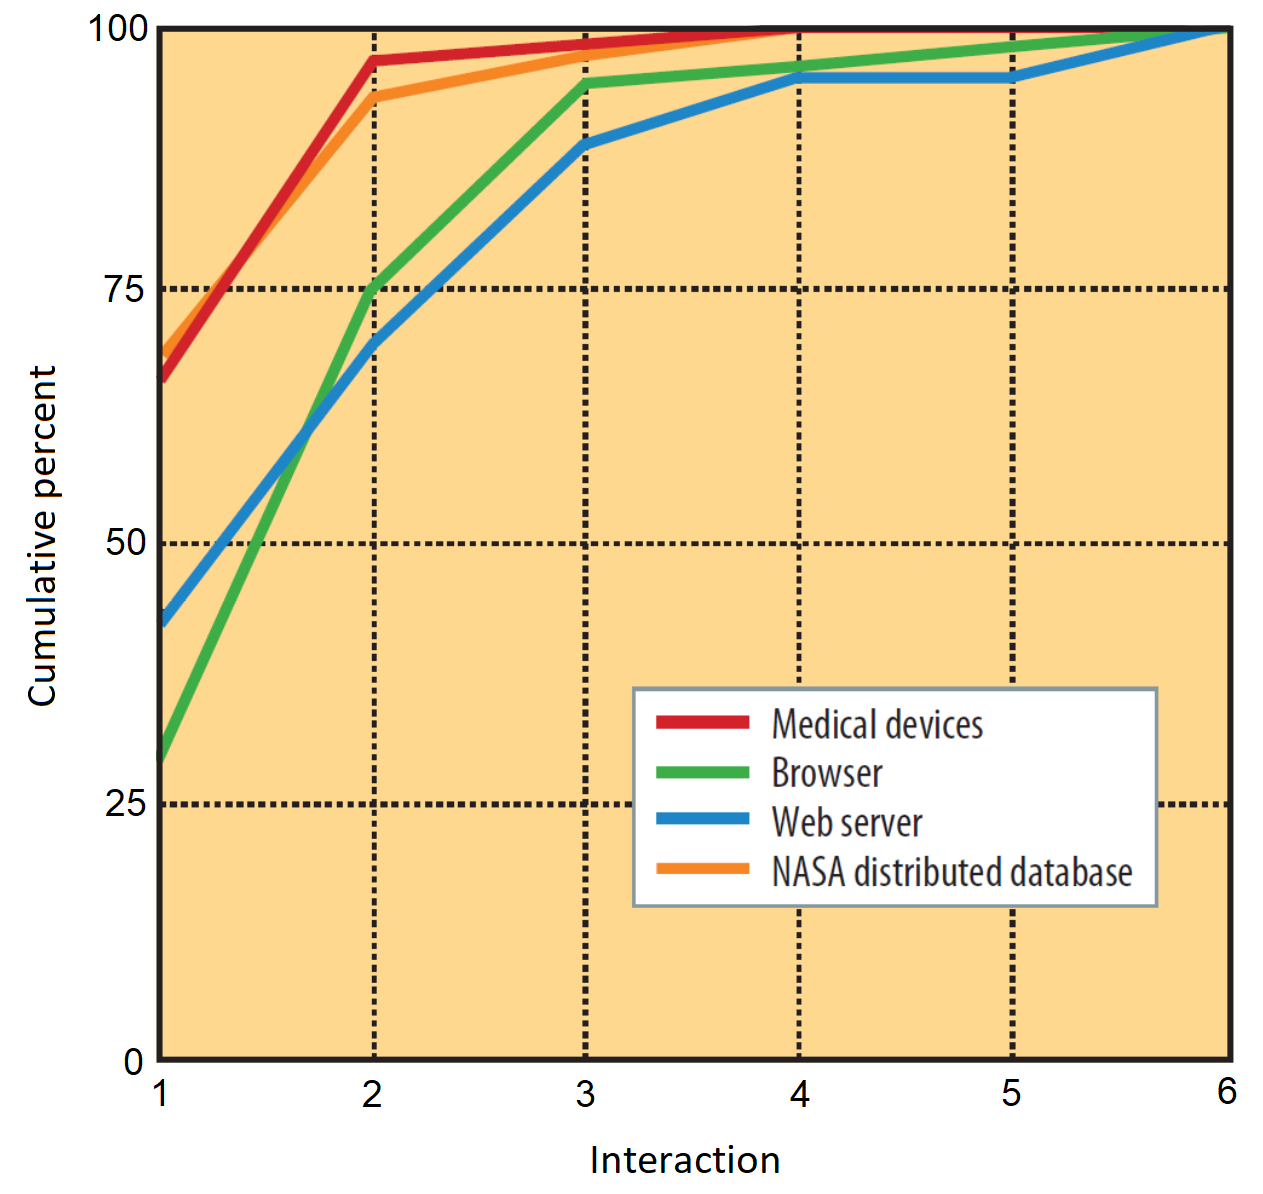
\includegraphics[width=0.6\textwidth]{obrazky-figures/Fault_graph2.png}
	\caption{Graf závisloti velikosti N a procent odhalených obsažených s systému. Graf je převzatý z \cite{4_IntroductionToCombinatorialTesting}}
	\label{fig_faultGraph}
\end{figure}

Toto zjištění problematiku kombinací značně zjednodušuje. Přesto pokrytí všech možných hodnot, byť jen 3 faktorů, je stále nereálné. Najít kompromis mezi počtem testů a množstvím odhalených chyb není snadný úkol. V následujících kapitolách jsou popsány přístupy, kterými lze tohoto cíle dosáhnout rozdělením vstupní domény do menších celků. 



\section{Definice základních pojmů}
\label{sec_definiceZakladnichPojmu}

V této kapitole jsou vysvětleny základní pojmy z oblasti testování, které jsou nezbytné k pochopení následujících kapitol. 


\begin{description}
	\item[SUT (System Under Test)] Testovaný systém nebo jeho část. 
	\item[Testování] Proces práce s SUT za určitých podmínek, zkoumání výsledků a následného hodnocení nějakého aspektu softwaru. 
	\item[Testovací sada] Soubor testovacích případů pro testovanou komponentu nebo testovaný systém. 
	\item[Kritérium pokrytí] Množina pravidel specifikující určité požadavky na testovací sadu. 
	\item[Pokrytí] Vyjádření míry, jak moc testovací sada zkoumá SUT. 
	\item[Testovací případ] Popis konkrétních akcí prováděných s určitou softwarovou komponentou a očekávané výsledky těchto akcí. 
	\item[Testovací požadavek] Vlastnost či funkce komponenty nebo systému, která by měla být ověřená alespoň jedním testovacím případem. 
	\item[Vstupní doména] Reprezentuje množinu všech možných vstupů SUT. 
	\item[Model vstupní domény] Abstrakce vstupu SUT. 
	\item[Charakteristika] Charakteristický rys či znak, dle kterého lze rozdělit vstupní doménu na třídy ekvivalence. 
\end{description}

\section{Rozklad vstupní domény}
\label{sec_RozkladVstupniDomeny}

Testování založené na rozkladu vstupní domény je přístup, který rozděluje množinu všech vstupních hodnot, \textit{vstupní doménu}, na menší celky stejného logického významu, \textit{bloky}. Pro zjednodušení se můžeme na testovaný systém (SUT) dívat jako na funkci, která má různé vstupní parametry, přičemž každý takový parametr má svoji vlastní doménu hodnot. 

Rozdělením domény se docílí toho, že z každého vzniklého bloku je možné zvolit pouze jednu reprezentativní hodnotu, která bude mít z pohledu testování stejný význam, jako jakákoliv jiná hodnota v rámci stejného bloku. Testovací sada následně vzniká jako kombinace reprezentativních hodnot všech parametrů SUT. Způsobu, jakým jsou tyto kombinace prováděny je věnována kapitola \ref{sec_KriteriumPokryti}. Díky tomuto přístupu je možné výrazným způsobem snížit množství potřebných testů bez negativního vlivu na jejich efektivitu. Nutno však podotknout, že účinnost takové testovací sady je silně závislá na zvolení vhodné charakteristiky, dle které k rozkladu dochází.  


\subsection*{Tvorba charakteristik}
\label{subsec_TvorbaCharakterisitk}

Při tvorbě charakteristik existují dva možné přístupy, jakými je možné se na parametry testovaného systému dívat. První z nich je založený na tom, že se na každý parametr nahlíží zvlášť, tudíž sémantika programu a vzájemná interakce parametrů se nebere v potaz. Výhodou tohoto přístupu je, že zvolení charakteristiky je velmi snadné a výsledné testy jsou i přesto velmi uspokojivé. Nevýhodou je však skutečnost, že některá funkcionalita SUT je závislá na kombinaci specifických hodnot několika parametrů. % Ta je z pohledu tohoto přístupu neotestovatelná skryá...

Druhý přístup je z hlediska náročnosti její tvorby mnohem komplikovanější, jelikož vychází z jistých znalostí SUT. Tester do charakteristik začleňuje i závislosti parametrů mezi sebou, čímž se eliminují nedostatky prvního přístupu.

Oba tyto přístupy však sdílí dvě kritéria, která musí každá charakteristika splňovat:
% Každá taková charakteristika musí splňovat následující kritéria:
\begin{enumerate}
    \item Sjednocení bloků $b$ z množiny všech bloků $B$ musí pokrývat celou vstupní doménu $D$ (úplnost).
		\begin{equation}
			\bigcup_{b\in B} b = D
		\end{equation}
    \item Jednotlivé bloky rozkladu jsou vzájemně disjunktní.
		\begin{equation}
			b_i \cap b_j = \emptyset,\qquad\textrm{(pro } i \neq j \textrm{ a } b_i, b_j \in B)
		\end{equation}
\end{enumerate}

Následující funkce demonstruje rozdíl těchto dvou přístupů. Uvažujme, že testujeme funkci, která zjišťuje, zda se nějaký element nachází v daném poli. Jak toto pole, tak hledaný element jsou funkci předány parametricky. 

% https://homel.vsb.cz/~s1a10/educ/EPubl/latex-docbook/ch06s06.html
\begin{lstlisting}[label={lst_example}]
public boolean findElement(List list, Object element)
// Effects: if list or element is null throw NullPointerException
//   else returns true if element is in the list, false otherwise
\end{lstlisting}

Použitím prvního přístupu, založeném na rozhraní, bude mít každý parametr své vlastní charakteristiky. Ukázka takového rozkladu pro parametr typu \textit{pole} je popsána tabulkou \ref{table_charakteristika1}. V tomto případě bylo k rozdělení vstupní domény využito speciálních hodnot či vlastností, které mohou nastat obecně pro libovolné pole. 
% Použitím prvního přístupu může vzniknou charkateristika pro pole popsaná tabulkou .

\begin{table}[h!]
\centering
\begin{tabular}{ |c|c|c| } 
 \hline
 Charakteristika & $b_1$ & $b_2$ \\ 
 \hline
 \textit{pole} je \textit{null} & True & False \\ 
 \textit{pole} je \textit{empty} & True & False \\ 
 \hline
\end{tabular}
\caption{Charakteristika pro přístup založený na rozhraní\cite{3_IntroductionToSWTesting}}
\label{table_charakteristika1}
\end{table}

Všimněme si, že každá charakteristika má v tomto příkladě pouze dva bloky, které indikují, zda daná vlastnost je či není splněna. Charakteristiky je samozřejmě možné vytvořit i jiným způsobem. Obecně vzato je však doporučeno tvořit spíše větší množství jednoduchých charakteristik než naopak, jelikož u komplikovanějších charakteristik je větší pravděpodobnost, že nedopatřením dojde k porušení jednoho z kritérií popsaných výše.\cite{3_IntroductionToSWTesting} 

Na druhém příkladu (tabulka \ref{table_charakteristika2}) jsou vypsány charakteristiky a jejich bloky s reprezentativními hodnotami, které jsou vytvořené s využitím jisté znalosti programu. Tester například uvažuje nad tím, kolik hledaných elementů se vlastně v poli může vyskytovat. Popřípadě, jestli se daný element v poli vůbec vyskytuje. 


\begin{table}[h!]
\centering
\begin{tabular}{ |c|c|c|c| } 
 \hline
 Charakteristika & $b_1$ & $b_2$ & $b_3$ \\ 
 \hline
 Počet nalezených prvků v poli  & $0$ & $1$ & Více než $1$ \\ 
 Prvek se nachází v poli na prvním místě & True & False & \\
 Prvek se nachází v poli na posledním místě & True & False & \\ 
 \hline
\end{tabular}
\caption{Charakteristika pro přístup založený na funkcionalitě}
\label{table_charakteristika2}
\end{table}

% Pro demonstraci dva příklady charakterisitk jsou použity pro funkci fin. V případě prvního přístupu, založeného na rozhraní, 

\subsection*{Rozklad do bloků}
\label{subsec_RozkladDomenyDoBloku}

Tester vytváří rozklad pro každou charakteristiku vstupní domény. Rozkladem vznikne sada bloků, kde každý blok obsahuje množinu hodnot, kterých může nabývat. Hlavním cílem této podkapitoly je vyřešení otázky, jakým způsobem by měly být jednotlivé bloky identifikovány, a jaká reprezentativní hodnota by měla být zvolena.

% Více bloků má za následek i více testů, které sice vyžadují více zdrojů, ale s pozitivním efektem na množství nalezených chyb.

Vycházíme-li z předpokladu o úplnosti vstupní domény, každý rozklad musí obsahovat jak validní, tak nevalidní hodnoty. Právě nevalidní hodnoty se dost často k rozkladu domény využívají. Příkladem je charakteristika popsaná v tabulce \ref{table_charakteristika1}, kde bylo využito nevalidního pole k vytvoření celé charakteristiky.

% Každý rozklad vstupní domény musí obsahovat jak validní tak nevalidní hodnoty. V opačném případě je porušeno pravidlo úplnosti. Příkladem je charakteristika popsaná v tabulce \ref{table_charakteristika1}, kde bylo využito nevalidního vstupu pole k vytvoření celé charakteristiky.

V příkladu z tabulky \ref{table_charakteristika2} se však již vycházelo z předpokladu, že pro první charakteristiku je nutné zvolit hodnoty, které vstupní doménu nějakým způsobem rozdělují a jejichž použití má z pohledu testování jiný význam. Princip, pomocí kterého jsou tyto hodnoty odhaleny, se nazývá analýza mezních hodnot. Ze zkušenosti vyplývá, že právě tyto hodnoty dost často způsobují defekty. 

Při tvorbě testovací sady pak chceme testovat dané rozdělující hodnoty, hodnotu o \textit{e} menší a hodnotu o \textit{e} větší. Kde \textit{e} symbolizuje rozdíl dvou po sobě jedoucích hodnot dané domény. Jako demonstrativní příklad si uvedeme funkcionalitu, které se jako parametr předává věk uživatele v očekávaném rozmezí 18-30 let. Mezními hodnotami tohoto programu jsou tedy 18 a 30. Speciálními pak \textit{infinite} a \textit{nan}.

Při tvorbě charakteristik se dost často využívá speciálních hodnot, kterých může parametr nabývat. Jedním takovým příkladem může být charakteristika pro parametr datového typu \textit{integer} a jeho speciální hodnota \textit{null} a \textit{nekonečno}. Současně rozklad musí počítat i s nevalidními hodnotami, případně hodnotami, které nějakým způsobem ovlivňují chování programu. 

Rozklad vstupní domény do bloků pak může vypadat následovně.\footnote{Dokumentace pro funkce isinf a isinf je dostupná na: https://www.mkssoftware.com/docs/man3/isinf.3.asp}

\begin{center}
\begin{tabular}{ |c|c| } 
 \hline
 Blok charakteristiky & Příklad hodnoty bloku \\ 
 \hline
 $x<18$ & $0$  \\ 
 $x=18$ & $18$  \\ 
 $x\in(18,30)$ & $25$  \\ 
 $x=30$ & $30$  \\ 
 $x>30$ & $102$  \\ 
 $isnan(x) == true$ & $null$  \\  
 $isinf(x) == true$ & $inf$  \\ 
 \hline
\end{tabular}
\end{center}


Pro tvorbu charakteristik se dost často využívá takzvaných \textit{kontrolních seznamů}. Kontrolní seznam obsahuje charakteristiky pro skoro až rutinní situace. Je vhodný pomocník při testování něčeho, co se často opakuje. Jedním takovým příkladem může být charakteristika pro parametr datového typu \textit{integer}, kde jsou předem nastaveny určité hodnoty (0, \textit{e}, \textit{-e}, největší hodnota, nejmenší hodnota). 




\section{Kritérium pokrytí}
\label{sec_KriteriumPokryti}
Předchozí podkapitola o rozdělení vstupní domény do bloků řešila problém s obrovským množstvím testů pro jednotlivé parametry, nezabývala se však způsobem, jakým budou hodnoty parametrů kombinovány mezi sebou.



Kritérium pokrytí umožňuje testerům se rozhodnout, jaké kombinace vstupů použít při testování, aby byly splněny požadavky na jeho kvalitu. Je samozřejmostí, že každý tester by chtěl vytvořit testovací sadu, která pokryje co největší množství kombinací, ideálně všechny. Ve většině případů to však není reálné a je potřeba najít kompromis mezi počtem testů a pravděpodobností, že taková testovací sada odhalí chybu vedoucí ke zlepšení kvality a spolehlivosti testovaného softwaru. Kritéria pokrytí tedy definují pravidla, která musí být splněna, aby bylo úsilí vynaložené pro testování SUT bráno jako dostatečné.  

Cílem je tedy vytvořit takovou testovací sadu, jejíž vlastnosti budou splněny alespoň jednou v každém testu. Pro snadné pochopení kritérií pospaných v této kapitole použijeme příklad, na kterém budou jednotlivá kritéria pokrytí znázorněna. Máme následující parametry typu \textit{char}, \textit{boolean} a \textit{string}, jejichž rozdělení vstupní domény do bloků s reprezentativními hodnotami je popsáno tabulkou \ref{table_kriteriaExample}. Na základě těchto hodnot budou demonstrovány jednotlivá kombinační kritéria pokrytí. 

% Pro vytvoreni testovacich sad zobrazenych v naseldujicichc tabulkach bylo vyuzito weboveho rozhrani nastroje Combine, ktery je dale popsat v kapitole X.

\begin{table}[h!]
\centering
\begin{tabular}{ |c|c|c| } 
 \hline
\textit{char} & \textit{boolean} & \textit{string} \\ 
 \hline
 M & True & aaa \\
 N & False & bbb \\
 O &  & ccc \\ 
 \hline
\end{tabular}
\caption{Jednoduchý příklad tří charakteristik, rozdělující vstupní doménu do bloků s reprezentativní hodnotou.}
\label{table_kriteriaExample}
\end{table}




\subsection*{All Combinations Coverage (ACoC)}
\label{subsec_acoc}

Jak již bylo zmíněno, jedním ze způsobů, jakým je možné kombinovat bloky charakteristik, je úplným pokrytím všech variant, které mohou vzniknout. Reprezentativní hodnota každého bloku jedné charakteristiky je kombinována s každým blokem ostatních charakteristik. Tento přístup je v praxi znám pod pojmem All Combinations Coverage. 

Obecně platí, že máme-li $n$ množin nějakých hodnot, pak kombinací všech jejich elementů mezi sebou vznikne $|M_1|*|M_2|*...*|M_n|$ možných variant, kde $M_n$ označuje množství prvků v množině. Tato operace je v matematice označována jako kartézský součin množin.

% Pro splňení tohoto kritéria se tedy musí provést kartézský součin všech charakteristik.
% Toto kritérium tedy není ničím jiným než Kartézským součinem.

Pro příklad daný tabulkou \ref{table_kriteriaExample} je množství potřebných testovacích případů dán výpočtem $3*2*3$. Pro úplné pokrytí je tedy zapotřebí minimálně $18$ testů, které jsou znázorněny tabulkou \ref{table_acoc}.

\begin{table}[h!]
\centering
\begin{tabular}{ |c|c c c| } 
 \hline
 & \textit{char} & \textit{boolean} & \textit{string} \\
 \hline
1 & M & true & aaa \\
2 & M & false & aaa \\
3 & M & true & bbb \\
4 & M & false & bbb \\
5 & M & true & ccc \\
6 & M & false & ccc \\
7 & N & true & aaa \\
8 & N & false & aaa \\
9 & N & true & bbb \\
10 & N & false & bbb \\
11 & N & true & ccc \\
12 & N & false & ccc \\
13 & O & true & aaa \\
14 & O & false & aaa \\
15 & O & true & bbb \\
16 & O & false & bbb \\
17 & O & true & ccc \\
18 & O & false & ccc \\
 \hline
\end{tabular}
\caption{Příklad testovací sady uspokojující kritérium ACoC}
\label{table_acoc}
\end{table}


\subsection*{Each Choice Coverage (ECC)}
\label{subsec_ecc}

Pro kritérium označované jako Each Choice Coverage platí, že nemusí docházet k žádným složitým kombinacím, nýbrž záleží pouze na tom, aby se každý blok každého oddílu vyskytnul v testovací sadě alespoň jednou. 

Minimální počet testovacích případů v testovací sadě je tedy roven počtu hodnot v doméně, která obsahuje nejvíce hodnot. V případě \ref{table_kriteriaExample} je tedy potřeba alespoň tří testů, aby byly pokryty všechny hodnoty \textit{char} a \textit{string}. Tyto testovací případy jsou znázorněny v následující tabulce.


\begin{table}[h!]
\centering
\begin{tabular}{ |c|c c c| } 
 \hline
 & \textit{char} & \textit{boolean} & \textit{string} \\
 \hline
1 & M & true & aaa \\
2 & N & false & bbb \\
3 & O & true & ccc \\
 \hline
\end{tabular}
\caption{Příklad testovací sady uspokojující kritérium ECC}
\label{table_ecc}
\end{table}

Nutno podotknout, že tohle je pouze jedno z možných řešení. Pro všechny kritéria v této kapitole platí, mimo kritérium All Combinations Coverage, že způsobů, jakým mohou být bloky jednotlivých charakteristik kombinovány, je více. 
% Některé algoritmy pro generování testovacích dat dokoncce větsi pocet.

% \begin{equation}
% \textrm{Max}^Q_{i=1}(B_i)
% \end{equation}


\subsection*{Pair-Wise Coverage (PWC)}
\label{subsec_pwc}

Kritérium Pair-Wise Coverage vyžaduje, aby reprezentativní hodnota každého bloku pro každou charakteristiku byla kombinovaná s hodnotou bloku každé jiné charakteristiky. Pokrytím všech dvojic u výše uvedeného příkladu třech oddílů s bloky $[M,N,O]$, $[True, False]$ a $[aaa,bbb,ccc]$, vzniknou následující páry.

% Vzhledem k výše uvednému příkladu tří oddílů s bloky $[M,N,O],[True, False],[aaa,bbb,ccc]$, pokrytím všech dvojic vzniknou následujicí kombinace:

\begin{table}[h!]
\centering
\begin{tabular}{ |c|l| } 
 \hline
Blok & Možné kombinační páry (dvojice) s ostatními bloky \\
 \hline
 M & $(M, True)$, $(M, False)$, $(M, aaa)$, $(M, bbb)$, $(M, ccc)$ \\
 N & $(N, True)$, $(N, False)$, $(N, aaa)$, $(N, bbb)$, $(N, ccc)$ \\
 O & $(O, True)$, $(O, False)$, $(O, aaa)$, $(O, bbb)$, $(O, ccc)$ \\
 True & $(True, aaa)$, $(True, bbb)$, $(True, ccc)$ \\
 False & $(False, aaa)$, $(False,bbb)$, $(False,ccc)$ \\
 \hline
\end{tabular}
\caption{Dvojice, které je potřeba pokrýt, aby bylo splněno PWC kritérium}
\label{table_pwc}
\end{table}

Všimněme si, že více takových dvojic je možné pokrýt pouze jedním testem. Například testovacím případem s hodnotami bloků $(M,True,aaa)$ dojde k pokrytí dvojic $(M,True)$, $(M, aaa)$ a $(True,aaa)$ najednou. Z této skutečnosti vyplývá, že existuje mnoho způsobů, jakými lze všechny dvojice zahrnout do testovací sady. Cílem je většinou najít takové kombinace, které vedou k co nejmenší testovací sadě. Ukázka jedné takové testovací sady je vyobrazena v následující tabulce.

\begin{table}[h!]
\centering
\begin{tabular}{ |c|c c c|l| } 
 \hline
 & \textit{char} & \textit{boolean} & \textit{string} & Pokryté dvojice \\
 \hline
1 & M & true & aaa & $(M, True)$, $(M, aaa)$, $(True, aaa)$ \\
2 & M & false & bbb & $(M, False)$, $(M, bbb)$, $(False,bbb)$ \\
3 & M & true & ccc & $(M, ccc)$, $(True, ccc)$ \\
4 & N & false & aaa & $(N, False)$, $(N, aaa)$, $(False, aaa)$\\
5 & N & true & bbb & $(N, True)$, $(N, bbb)$, $(True, bbb)$ \\
6 & N & false & ccc & $(N, ccc)$, $(False,ccc)$ \\
7 & O & true & aaa & $(O, True)$, $(O, aaa)$ \\
8 & O & false & bbb & $(O, False)$, $(O, bbb)$\\
9 & O & true & ccc & $(O, ccc)$  \\
 \hline
\end{tabular}
\caption{Příklad testovací sady uspokojující kritérium PWC}
\label{table_resultpwc}
\end{table}

Testování využívající kritérium pokrytí všech dvojic je velmi efektivní. Jeho efektivita vyplývá především ze skutečnosti, že většina softwarových selhání je způsobena jedním, maximálně dvěma parametry.

% \begin{equation}
% (\textrm{Max}^Q_{i=1}(B_i)) * (\textrm{Max}^Q_{j=1}(B_j)),\qquad\textrm{pro } i \neq j
% \end{equation}


% 239
\subsection*{T-Wise Coverage (TWC)}
\label{subsec_twc}

T-Wise Coverage, taktéž označováno jako N-Wise, je jakýmsi rozšířením předchozího kritéria pokrývající všechny dvojice bloků. Rozšíření spočívá v tom, že kritérium není zaměřeno pouze na dvojice, ale na celé n-tice. Tento stupeň $N$, případně $T$, udává sílu či násobnost kombinací, které je potřeba v testovací sadě splnit. Pair-Wise kritérium lze tedy považovat jako T-wise s kombinační silou $T=2$. 

Je evidentní, že vytvářet čtveřice v našem příkladu \ref{table_kriteriaExample} s pouze třemi oddíly, je nereálné. Síla kombinací proto nesmí přesáhnout počet oddílů SUT. V případě, kdy je počet oddílů stejný, jako násobnost jeho kombinací $T$, pak takto definované kritérium je ekvivalentní kritériu všech kombinací popsaných v \ref{subsec_acoc}. 

% se prakticky jedná o pokrytí všech kombinací. Současně V našem příkladu z X je evidentní, že vytvářet čtvečice ze 3 oddílů není možné.
Z této logiky vyplývá, že čím větší kombinační síla, tím větší a úspěšnější bude i výsledná testovací sada. Jak již však bylo naznačeno v podkapitole \ref{subsec_pwc}, existuje obrovské množství způsobů, jakými lze tuto sadu sestavit. Cílem je většinou najít takové kombinace, které vedou k co nejmenší testovací sadě. To je však obzvláště pro $T>3$ velmi komplexní problém, kterým se v této práci nebudeme zabývat. Tato problematika je částečně rozebrána v bakalářské práci Radima Červinky \cite{1_Combine}. 



\subsection*{Base Choice Coverage (BCC)}
\label{subsec_BCC}
% Pro všechna předešlá kritéria platí, že vyžadují, aby byly splňeny určitá kritéria bez ohledu na to, jake hodnoty by se měly kombinovat prioritně. Base Choice Coverage do kombinací přinaší malou, ale zásadní informaci o tom, jaká hodnota je z pohledu testování nejpodstatnější. V praxi to může být například hodnota, která se ve výsledném systému bude používat nejčastěji.
Pro všechna předešlá kritéria platí, že vyžadují, aby byly splněny určitá pravidla bez ohledu na to, jaké hodnoty by se měly kombinovat prioritně. Base Choice Coverage do výsledných kombinací přináší malou, ale zásadní informaci o tom, jaké bloky jsou z pohledu testování nejpodstatnější. Tyto bloky se označují jako \textit{bázové}. V praxi se může například jednat o blok, který se v testovaném systému bude používat nejčastěji. 

% V prvním kroku je tedy potřeba zvolit bázový blok pro každý oddíl SUT. 
Nejdříve je tedy pro každý oddíl SUT zvolen bázový blok. Pro demonstraci vezměme v úvahu příklad z předchozích kritérii, který je zobrazen na tabulce \ref{table_bcc} vlevo - s bázovými bloky označenými tučně. Prvním vytvořeným testovacím případem pak bude kombinace těchto bázových bloků - $(M, True, aaa)$. Následné testovací případy musí splňovat podmínku, že každý nebázový blok je v kombinaci se všemi bázovými bloky v ostatních oddílech. Výsledná testovací sada našeho příkladu je pak vyobrazena v následující tabulce vpravo. 

% Jinými slovy, V našem příkladu musí být v každém testu alespoň dva bázové bloky a třetí parametr bude doplňen nebázovým
% Následné testovací případy musí splňovat, že pouze jeden blok v testovacím případu bude nebázový.
% test, který se bude skládat pouze z kombinace těchto bázových bloků.

% Následné testy a jejich množství se odvíjí od nebázových bloků, přičemž k tomu, aby Base Choice Coverage kritérium bylo splňeno, každý nebázový blok pak musí být v kombinaci se všemi bázovými v ostatních oddílech.

% Uvažujme, že v první blok z každého našeho oddílu v uvedeném příkladu budeme považovat za bázový, pak bázový test je $(M, True, aaa)$ a následné testy by byly uvedeny v tabulce společně s bázovýmí.

\begin{table}[h!]
\centering
\begin{tabular}{ |c|c|c| } 
 \hline
\textit{char} & \textit{boolean} & \textit{string} \\ 
 \hline
 \textbf{M} & \textbf{True} & \textbf{aaa} \\
 N & False & bbb \\
 O &  & ccc \\ 
 \hline
\end{tabular}
\quad
\begin{tabular}{ |c|ccc| } 
 \hline
& \textit{char} & \textit{boolean} & \textit{string} \\ 
\hline
1 & \textbf{M} & \textbf{True} & \textbf{aaa} \\
2 &  \textbf{M} & \textbf{True} & bbb \\
3 &  \textbf{M} & \textbf{True} & ccc \\
4 &  \textbf{M} & False & \textbf{aaa} \\
5 &  N & \textbf{True} & \textbf{aaa} \\
6 &  O & \textbf{True} & \textbf{aaa} \\
 \hline
\end{tabular}
\caption{Příklad se zvýrazněnými bázovými bloky (vlevo). Příklad testovací sady uspokojující kritérium PWC (vpravo)}
\label{table_bcc}
\end{table}


Existuje i alternativa tohoto kritéria, která umožňuje zvolit více bázových bloků jedné charakteristiky. Takové kritérium je označováno jako Multiple Base Choice Coverage (MBCC).
% V případě, že chceme kritérium rozšířit o více bázových bloků, se zabývá Multiple Base Choice Coverage, pro který platí, že více, ale alespoň jeden bázový blok je určen pro každou charakteristiku a bazove testy jsou formovány použitím bázových bloků každé cahrakteristiky alespoň jednou

\chapter{Rozhraní pro programování aplikací} 
\label{ch_API}

Jak již bylo zmíněno, v této práci se budeme zabývat kombinačnímu testováním zaměřené na API (Application Programming Interface), neboli \textit{rozhraní pro programování aplikací}. Předtím, než se pustíme do samotného návrhu aplikace Suiter, která bude pro toto testování generovat testovací sady, si musíme ujasnit, co to vlastně API je, jakým způsobem funguje, a jaké existují přístupy pro jeho realizaci. % přístupy vzhledem k použité architekruře se používají. V neposlední řadě si povíme pár slov o tom, jakým způsobem se dá toto rozhraní testovat.

Rozhraní pro programování aplikací lze definovat jako nástroj zapouzdřující množinu určitých metod a funkcí, které jsou poskytované třetím stranám. V současnosti je pojem API většinou spojován s webovými službami, které jsou dostupné využitím komunikačního protokolu HTTP. Pojmy API a webové služby však nejsou synonyma a API je využíváno například i na úrovni operačních systémů. Tato práce je však zaměřená výhradně na testování API spojených s webovými službami využívající protokol HTTP. 

Rozhraní pro programování aplikací má mnoho využití. Jedním z nich je integrování již existujících softwarových řešení do vlastních projektů. Příkladem může být API pro Google Mapy, které umožňuje využívat určité jeho funkce bez nutnosti jakékoliv implementace. 

Většina rozhraní pro programování aplikací však není veřejně dostupná a mnoho komplexních systémů jej využívá pouze pro vzájemnou komunikaci uvnitř interního systému.
% pro vzájemnou komunikaci uvnitř tohoto interního systému. Jeho funkcionalita je tedy pro veřejnost skryta. 


\section{Webové služby}
\label{sec_webove sluzby}
Jak již bylo nastíněno na začátku této kapitoly, mezi API a webovými službami je malý, ale podstatný rozdíl. Webové služby dle definice vyžadují, aby komunikace probíhala po síti. Jinými slovy, každá webová služba je současně i API, jelikož poskytuje aplikační data nebo její funkcionalitu, ale ne každé API musí být i webovou službou. 

% https://www.w3.org/TR/ws-arch/#whatis
Dle definice popsané v \cite{W3C_web_services_architecture} organizací W3C (World Wide Web Consortium), jsou webové služby softwarovým systémem, sloužící k podpoře vzájemné komunikace dvou strojů v síti. Rozhraní těchto služeb je popsané ve strojově zpracovatelném formátu WSDL (Web Services Description Language). Ostatní systémy komunikují s webovou službou předepsaným způsobem pomocí SOAP zpráv, které jsou serializovány pomocí značkovacího jazyka XML a typicky transportovány pomocí HTTP protokolu. 

Existují však i jiné způsoby komunikace s webovou službou. Je jím například komunikace založená na operacích CRUD (Create, Read, Update, Delete), realizovaná pomocí Representational State Transfer architektury, zkráceně REST, a transportního protokolu HTTP. Tyto pojmy budou detailněji popsány v následujících kapitolách. 
% jako Representational State Transfer (REST) pomocí protokolu HTTP.

\section{Simple Object Access Protocol}
\label{sec_SOAP}
% https://www.guru99.com/soap-simple-object-access-protocol.html

Simple Object Access Protocol, zkráceně SOAP, je protokol určený pro výměnu zpráv v distribuovaných systémech, založených na formátu XML. První verze protokolu byla vydána už v roce 1999 a byla vyvinuta jako nástupce předchozího XML-RPC.

Z původní definice webových služeb vyplývá, že každá webová služba je popsána pomocí Web Service Description Language, neboli WSDL. Jedná se o jazyk pro popis funkcí, jenž daná webová služba nabízí. Současně popisuje i vstupy a výstupy těchto funkcí. Zjednodušeně tedy WSDL definuje, jakou funkcionalitu daná webová služba nabízí a jakým způsobem je možné její funkce použít.

Další technologii, kterou SOAP protokol může využívat, je UDDI - \textit{Universal Description, Discovery and Integration}. Jedná se o mechanismus pro registrování a vyhledávání webových služeb. 

Vzájemné vztahy mezi těmito třemi technologiemi jsou zachycené na obrázku \ref{fig_UkazkaKomunikaceWebServices}. Simple Object Access Protocol však není ani na jedné z těchto technologií přímo závislý a dokáže fungovat i samostatně. WSDL a UDDI vznikly až po představení SOAP protokolu s cílem zjednodušit práci s tímto protokolem. 

\begin{figure}[hbt]
	\centering
	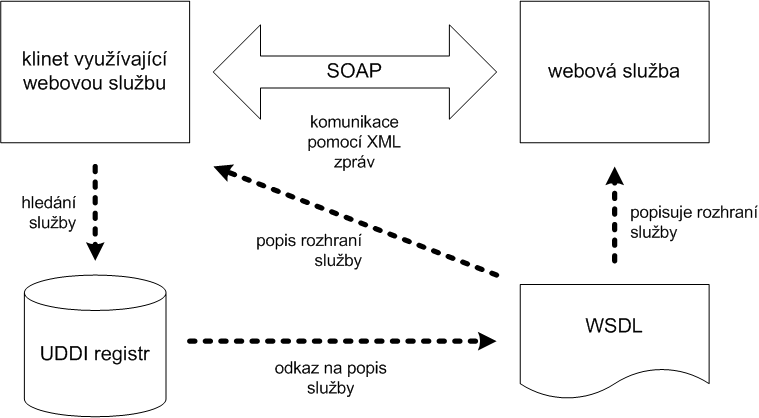
\includegraphics[width=0.8\textwidth]{obrazky-figures/komunikace-webservices.png}
	\caption{Vztah tří základních technologií (SOAP, WSDL, UDDI). Zdroj: \cite{Kosek_InteligentniPodporaNavigace}}
	\label{fig_UkazkaKomunikaceWebServices}
\end{figure}

SOAP umožňuje zaslání XML zprávy mezi dvěma aplikacemi a pracuje tedy na principu peer-to-peer. Jedna aplikace pošle v XML zprávě požadavek jiné aplikaci, ta ho obslouží a výsledek zašle v další zprávě zpět původnímu iniciátorovi komunikace. Jednotlivé XML zprávy jsou většinou doručovány použitím HTTP protokolu.\cite{Kosek_InteligentniPodporaNavigace}

Každá XML zpráva se skládá ze tří částí, kde kořenovým elementem je takzvaná obálka (envelope). Jak samotný název napovídá, obálka zapouzdřuje celou SOAP zprávu a jsou v ní obsaženy dva další elementy - nepovinnou hlavičku (header) a tělo zprávy (body). Hlavička se používá pro přenos pomocných informací pro zpracování zprávy. Příkladem může být identifikace uživatele, autentizační informace a podobně.\cite{Kosek_InteligentniPodporaNavigace} 

Nejdůležitější částí každé XML zprávy je však její tělo, v němž se přenášejí informace identifikující volanou službu a předávané parametry, které služba vyžaduje. Následující ukázka představuje volání jednoduché metody \textit{GetStockPrice} pomocí protokolu HTTP. Ukázka byla převzata z \cite{w3schools}, jejíchž první řádky budou vysvětleny v kapitole \ref{chap_HTTP}.

% \lstset{frame = single}

\begin{lstlisting}[frame=single]
POST /InStock HTTP/1.1
Host: www.example.org
Content-Type: application/soap+xml; charset=utf-8
Content-Length: X

<?xml version="1.0"?>
<soap:Envelope
xmlns:soap="http://www.w3.org/2003/05/soap-envelope/"
soap:encodingStyle="http://www.w3.org/2003/05/soap-encoding">
<soap:Body xmlns:m="http://www.example.org/stock">
  <m:GetStockPrice>
    <m:StockName>IBM</m:StockName>
  </m:GetStockPrice>
</soap:Body>
</soap:Envelope>
\end{lstlisting}

% Zpráva SOAP je XML skládající se ze 3 částí - obálky, hlavičky a těla. Obálka je nejvyšší element XML dokumentu 

\section{Representational State Transfer}
\label{sec_REST}
% Pojem \textit{zdroj} je v obecném smyslu použit pro cokolik, co může být identifikováno pomocí URI.

% https://tools.ietf.org/html/rfc3986
Representational State Transfer, zkráceně REST, je architektonický styl určující pravidla, potřebná k přenosu reprezentativního stavu zdroje v distribuovaných systémech. Architektura REST byla navržena a popsána v roce 2000 v disertační práci \cite{Roy} Roye Fieldinga, který je současně i jedním ze spoluzakladatelů protokolu HTTP, jehož verze HTTP/1.1 byla s architekturou REST vyvíjena souběžně.

Rozhraní REST je použité pro jednotný a snadný přístup ke zdrojům. Pojem \textit{zdroj} je v obecném smyslu použit pro cokoli, co může být identifikováno pomocí URI. REST je tedy na rozdíl od SOAP orientován datově, nikoli procedurálně. 

% https://is.muni.cz/th/uo42j/navrh-a-implementace-restovych-rozhrani.pdf
Podobně jako SOAP je i REST architektura nezávislá na konkrétní implementaci komunikačního protokolu. Definuje pouze konkrétní podmínky, které musí být splněny, aby webová služba mohla být označena jako \textit{RESTful}. V současných webových službách se dá však protokol HTTP považovat za standard pro přenos zpráv a použití jiného protokolu je poměrně výjimečné. Protokol HTTP je podrobněji popsán v kapitole \ref{chap_HTTP}. 

Tato architektura se používá pro komunikaci mezi dvěma nezávislými stanicemi, jejichž data se typicky přenášejí pomocí serializačních formátů, jako například JSON nebo XML. Za RESTful rozhraní můžeme považovat taková rozhraní, která splňují následující podmínky:\cite{Schmidl} 
% Tyto omezení jsou podrobněji vysvětleny v následujících podkapitolách.
\begin{itemize}
  \item Fungují na modelu klient-server.
  \item Jsou bezstavové.
  \item Využívají uniformní přístup ke zdrojům.
  \item Podporují správu mezipaměti.
  \item Jsou vrstvenná.
\end{itemize}


\subsection*{Model klient-server}
\label{subsec_ModelKlientServer}

Prvním omezením je požadavek, aby komunikace probíhala podle architektonického stylu klient-server. Server, nabízející sadu služeb, naslouchá požadavkům zasílaných klientem. Poté tyto požadavky provede, případně zamítne, a pošle klientovi zpět odpověď. Vzájemná komunikace je znázorněna na obrázku \ref{fig_KlientServerModel}. 

\begin{figure}[hbt]
	\centering
	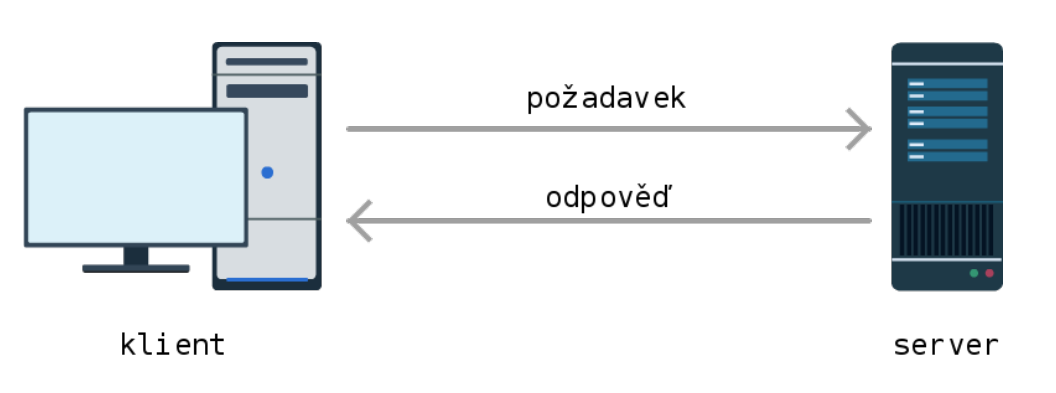
\includegraphics[width=0.6\textwidth]{obrazky-figures/Klient-server.png}
	\caption{Klient-server model. Zdroj: \cite{Schmidl}}
	\label{fig_KlientServerModel}
\end{figure}

Oddělením uživatelského rozhraní a datového úložiště, se zjednodušuje možná portace tohoto rozhraní napříč více platformami. Současně dochází i k snadnější škálovatelnosti na straně serveru, jelikož jeho komponenty mohou být jednodušší. Zásadní výhodou tohoto přístupu však je možnost vyvíjet jednotlivé komponenty odděleně. A to jak na straně klienta, tak na straně serveru.\cite{Roy} 


\subsection*{Bezstavovost}
\label{subsec_Bezstavovost}

Jedním z velmi limitujících požadavků na webové služby, dodržující REST architekturu, je jejich bezstavovost. Současně se však jedná o jednu z hlavních myšlenek této architektury. Klientův požadavek musí obsahovat veškeré informace, které jsou potřebné k pochopení kontextu zprávy. Udržení relace je tedy ponecháno čistě na straně klienta.

Toto omezení dává webové službě jisté užitečné vlastnosti, týkající se především její viditelnosti, spolehlivosti a škálovatelnosti. Systém monitorující požadavky klientů se tak nemusí zaobírat předešlými zprávami za účelem určení souvislostí jednotlivých požadavků. Spolehlivost je zvýšena díky snadnějšímu odhalování a zotavování se z poruch. Jeho škálovatelnost pak díky toho, že si server nemusí ukládat stav komunikace, a tím je možné používané prostředky rychleji uvolňovat.\cite{Roy}

Volba architektury, podléhající požadavku na její bezstavovost, má však i negativní dopady. Jedním z nich je skutečnost, že při více požadavcích od stejného klienta, budou zprávy obsahovat repetitivní informace. Tím je zvýšena režie potřebná k jejich obsloužení, a především dochází ke snížení výkonu sítě.  

Kromě toho, přenecháním zodpovědnosti na pamatování stavu aplikace na straně klienta se snižuje kontrola serveru nad konzistentním chováním aplikace, jelikož se stává závislou na správné implementaci na straně klienta.


\subsection*{Uniformní rozhraní}
\label{subsec_UniformniRozhrani}

Ústředním prvkem, který odlišuje architektonický styl REST od ostatních síťových stylů, je jeho důraz na jednotné rozhraní. Každé takové rozhraní musí splňovat určitá omezení. Jedno z nich souvisí s identifikací zdroje, jeho reprezentací, a definicí toho, co si pod pojmem zdroj vlastně můžeme představit. 

Veškeré informace, které je možné pojmenovat, se v REST architektuře dají požadovat za \textit{zdroj} a každý takový zdroj musí být identifikovatelný pomocí URI. Zdrojem tedy v praxi může být dokument, obrázek, případně i objekt či kolekce jiných zdrojů.\cite{Roy}

% https://is.muni.cz/th/u2ra1/thesis.pdf
Fielding ve své práci \cite{Roy} představil koncept \textit{Hypermedia jako aplikační stav}, který se později ujal pod zkratkou HATEOAS z anglického Hypermedia as the Engine of Application State. Pojem \textit{hypermédium} označuje média, která jsou propojena referencemi, taktéž označovány jako hyperlinky, s jinými médii. Uživatel se tak může následováním hyperlinku dostávat k dalším informacím nebo vracet zpět. Jinými slovy, uživateli stačí jediná informace, vstupní URI, pomocí které je schopen dynamicky získat veškeré ostatní informace a operace, které nad zdroji může provádět. 


\subsection*{Správa mezipaměti}
\label{subsec_SpravaMezipameti}

Pro zvýšení efektivity komunikace mezi klientem a serverem je zavedeno omezení definující správu mezipaměti, neboli \textit{caching}. Toto omezení vyžaduje, aby data v odpovědi byla implicitně nebo explicitně označena, zda jsou kešovatelná či nikoliv. V případě, že odpověď byla uložená do mezipaměti, má uživatel možnost použít tuto odpověď i později bez nutnosti opětovného se dotazování serveru.

Výhodou přidání správy mezipaměti je, že je možné částečně nebo úplně eliminovat některé interakce, což vede k vyšší účinnosti a škálovatelnosti. Uživatel tím pak ocení snížení průměrné odezvy řady interakcí, jako například načítání webové stránky. 

Nevýhodou však je, že mezipaměť může snížit spolehlivost, pokud se zastaralá data v mezipaměti výrazně liší od dat, která by byla získána novým požadavkem odeslaným na server.


\subsection*{Rozdělení do vrstev}
\label{subsec_RozdeleniDoVrtev}

Za účelem dalšího zlepšení chování webových služeb jsou přidány požadavky na vrstvení systému. Požadovaný model klient-server \ref{subsec_ModelKlientServer} již zavádí určité rozložení funkcionality. Přidáním dalších vrstev však dochází k rozdělení komplexního systému do hierarchické struktury. Každá vrstva takové struktury pak poskytuje služby vrstvě nad ní a využívá služeb vrstvy pod ní.
% podřadné vrstvy.
% sodn9

Mezi klienta a server je tedy možné vložit prostředníky. Klient poté není schopný rozeznat, zda komunikuje přímo se serverem či pouze s jeho prostředníkem. To slouží k lepšímu rozložení napříč celé sítě. Málo používaná funkcionalita pak může být přesunuta do prostředníka s cílem zjednodušit a zpřehlednit serverovou implementaci. Případně se může využít prostředníků k ulehčení práce jednotlivých komponent při velkém zatížení. 

Větší množství vrstev a s tím spojené i množství potřebné komunikace však vede k negativnímu vlivu na odezvu celého systému. Tato nevýhoda se však dá kompenzovat využitím správy mezipaměti z předchozí podkapitoly.

\subsection*{Kód na vyžádání}
\label{subsec_CodeOnDemand}

Toto volitelné omezení, známější pod anglickým pojmem Code on demand, zajišťuje, že v rámci komunikace není přenos omezen pouze na data, ale server poskytuje klientovi i možnost stáhnout si spustitelný kód formou skriptu, který se následně spouští na straně klienta. Klient tak nemusí implementovat veškerou funkcionalitu, ale některé funkce mohou být uloženy na serveru a zaslány uživateli v případě jeho vyžádání.

To však může způsobit problémy z hlediska bezpečnosti. Klient nemá jistotu, že serveru může důvěřovat, jelikož z obdrženého skriptu není možné určit, co po spuštění způsobí. Z tohoto důvodu je kód na vyžádání, jediné volitelné omezení REST architektury.



\section{Hypertext Transfer Protocol}
\label{chap_HTTP}

Hypertext Transfer Protocol, neboli HTTP, je internetový protokol pro distribuované systémy operující na aplikační vrstvě. Původně byl navržen pouze k přenosu hypertextových dokumentů HTML, dnes má však mnohem větší využití. Běžně používaná verze HTTP/1.1, definována v RFC 2616, umožňuje využitím MIME (Multipurpose Internet Mail Extensions) ve zprávách zasílat i text v jiném než standardním kódování. Tím je protokolu umožněn například i přenos binárních dat, obrázků či dokonce zvuku. Nejnovější verzí je aktuálně HTTP/2, která je s hojně rozšířenou verzí HTTP/1.1 zpětně kompatibilní.\cite{rfc2616}


Protokol HTTP funguje na principu dotazů a odpovědí mezi klientem a serverem. Jedná se o bezstavový protokol, kde jednotlivé požadavky klienta nejsou nijak svázány a server si neukládá relaci o jejich předchozí komunikaci. Klient nejdříve zašle požadavek na server, ten ho vyhodnotí, a pošle zpět zprávu s odpovědí. V případě dalšího požadavku se pak celá komunikace opakuje stejným způsobem, tedy bez znalosti serveru o kontextu předchozí komunikace.

Každá taková HTTP komunikace se tedy skládá pouze ze dvou typů zpráv: z dotazu a z odpovědi. Obě tyto zprávy mají stejnou strukturu a liší se pouze jejím obsahem. Každá zpráva je strukturována do čtyř částí: prvního řádku označovaným jako \textit{start-line}, části obsahující hlavičky, prázdného řádku a případného těla zprávy. Na obrázku \ref{fig_UkazkaKomunikace} je zobrazen příklad HTTP komunikace včetně rozdělení zpráv do těchto částí.

\begin{figure}[hbt]
	\centering
	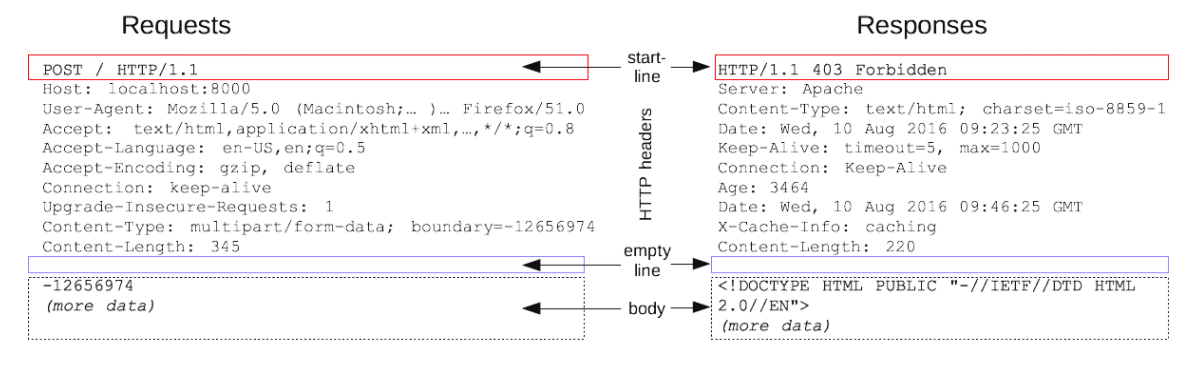
\includegraphics[width=1\textwidth]{obrazky-figures/RequestsResponse.png}
	\caption{Ukázka HTTP komunikace. Vlevo je zpráva požadavku, vpravo jeho odpovědi. Zdroj: \cite{mozilla}}
	\label{fig_UkazkaKomunikace}
\end{figure}

% Pomocí příkladu \ref{fig_UkazkaKomunikace} budou tyto části vysvětleny budou na nich ukázány
% a ukážeme si rozdíly mezi obsahem požadavku a obsahem odpovědi. \ref{rfc2616}

Začněme prvním řádkem, který je klíčový pro rozlišení, zda se jedná o dotaz nebo odpověď. Dle RFC specifikace je tento řádek nazýván jako \textit{start-line} a v případě, že se jedná o dotaz, je možné tento řádek označit jako \textit{Request-Line}, v případě odpovědi pak jako \textit{Status-Line}. Pomocí tohoto řádku je tedy možné na první pohled určit, zda daná zpráva reprezentuje dotaz či odpověď. 

Za tímto řádkem následuje několik řádků hlaviček, které umožňují klientovi a serveru předat určité dodatečné informace o zaslané zprávě. Každá hlavička je definovaná jménem a hodnotou, oddělenými dvojtečkou. Existuje více typů hlaviček, rozdělených dle jejich kontextu užití. Některé hlavičky se používají výhradně pro specifikování zprávy požadavku, jiné naopak pouze pro jeho odpovědi. Další skupina pak nese informaci o těle HTTP zprávy, jako například velikost jeho obsahu, případně jaké kódování je použito. Odesílateli zprávy je také umožněno definovat si i své vlastní hlavičky, většinou označovaných prefixem 'X-'. Ukázka některých, často používaných hlaviček, společně s jejich významem je zobrazena v tabulce \ref{table_UkazkaHlavice}


\begin{table}[h]
\centering
% \begin{tabular}{ |p{0.25\linewidth} | p{0.2\linewidth} | p{0.45\linewidth}| } 
% \begin{tabular}{ |c|c|c| } 
\begin{tabular}{ |p{0.25\linewidth} | p{0.65\linewidth}| }
 \hline
Hlavička & Popis \\ 
 \hline
Allow  & Identifikuje, které z HTTP metod server podporuje. \\
\hline
Authorization & Obsahuje autentizační informace uživatele.  \\
 \hline
Connection & Určuje, zda síťové spojení zůstane otevřené i po dokončení aktuálního požadavku. \\
 \hline
Content-Encoding & Určuje kódování zasílaných dat v těle zprávy. \\
 \hline
Content-Language & Specifikuje jazyk, pro který je určitá část obsahu určena. \\
 \hline
Content-Type & Označuje MIME typ média těla přenášené zprávy.  \\ 
 \hline
Content-Length & Specifikuje velikost těla zprávy v bajtech. \\
 \hline
Date & Definuje datum a čas, kdy zpráva vznikla. \\
 \hline
Expires & Definuje datum a čas, po kterém se data mají považovat za neplatná. \\
 \hline
Host & Určuje server a číslo portu, na které má být požadavek poslán. \\
 \hline
Server & Předává informaci o serveru, který generoval odpověď. \\
 \hline
\end{tabular}
\caption{Příklady často používaných HTTP hlaviček}
\label{table_UkazkaHlavice}
\end{table}


Třetí část je na první pohled jen málo důležitá, hraje však ve zprávě významnou roli. Odděluje totiž definici hlaviček od poslední části, samotného těla HTTP zprávy. Ne všechny zprávy však toto tělo obsahují. Příkladem může být volání metody HEAD, popsané v tabulce \ref{table_HTTPmethods}.
% V určitých případech, jako například volání metody HEAD.


\subsection*{HTTP požadavek}
% která má být nad daným zdrojem použita
% Pojem \textit{zdroj} bude podrobněji vysvětlen u REST architektury.
Zpráva klienta dotazující se na server zahrnuje v rámci prvního řádku HTTP zprávy klíčové slovo popisující konkrétní použitou metodu, následovanou identifikátorem zdroje a použitou verzí protokolu HTTP. Dvě ukázky, jak takové prvních řádky HTTP požadavku mohou vypadat, jsou zobrazeny na následujícím příkladu: 

\begin{center}
\begin{tabular}{c}
\begin{lstlisting}
GET https://www.vutbr.cz/ HTTP/1.1
POST 127.0.0.1:5000 HTTP/1.1
\end{lstlisting}
\end{tabular}
\end{center} 

Pro identifikaci zdroje na serveru se používá Uniform Resource Identifier, zkráceně URI. Jedná se o nadřazený pojmem pro Uniform Resource Name (URN) a pro Uniform Resource Locator (URL). URN specifikuje konkrétní zdroj, ale ne cestu k jeho dosažení. Ta je definovaná pomocí URL. V rámci komunikace mezi klientem a serverem se však s pojmem URN moc často nesetkáme, a tudíž jsou pojmy URL a URI dost často zaměňovány a oba lze považovat za způsob, jakým lokalizovat daný zdroj na internetu.\cite{rfc3986} 

% \begin{figure}[hbt]
% % https://www.guru99.com/url-vs-uri-difference.html
% 	\centering
% 	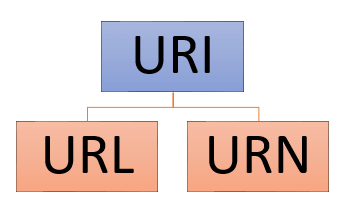
\includegraphics[width=0.6\textwidth]{obrazky-figures/URI_URL_URN.png}
% 	\caption{Vzájemný vztah URI, URL a URN. Zdroj: \cite{guru99}}
% 	\label{fig_URI_URL_URN}
% \end{figure}

URL musí být na prvním řádku zadaná absolutní cestou. Výjimkou je situace z příkladu \ref{fig_UkazkaKomunikace}, kde je cesta na prvním řádku zadaná relativně vzhledem k serveru, jenž je specifikován pomocí HTTP hlavičky \textit{Host}. Ve všech zprávách však musí být cesta ke zdroji přesně identifikována. 
\newpage
Obecně vzato má každá URL adresa následující tvar: 
% kde je cesta na prvním řádku zadná relativním způsobem a její server je specifikován pomocí hlavičky \textit{Host}
\begin{lstlisting}
Protokol://[Uzivatel[:Heslo]@]Host[:Port][/Cesta][?Parametr[&DalsiParametr]]
\end{lstlisting}

% \begin{center}
% \begin{tabular}{c}
% \end{tabular}
% \end{center}
% pro identifikaci konkrétního zdroje nesetkáme a tudíž jsou pojmy URL a URI dost často zaměňovány
% protokol://[uzivatel[:heslo]@]server[:port]/[cesta/][soubor]

Hranatými závorkami jsou označovány části adresy, které jsou z hlediska její úplnosti nepovinné. První část identifikuje protokol, který má být pro přenos použit. Následuje dnes již zastaralá, a ne příliš bezpečná forma autentizace uživatele. Poté je v URL adrese specifikováno doménové jméno nebo IP adresa serveru, na kterém se zdroj nachází, případně pak i port, na kterém server přijímá požadavky. Následně už je specifikovaná přímo konkrétní cesta ke zdroji. V případě, že je serveru potřeba předat nějaké dodatečné informace, je využito parametrů dotazu. Jedná se o proměnné hodnoty oddělené ampersandem a od zbytku URL otazníkem. 
% Jednotlivé parametry jsou v URL odděleny znakem ampersandu.

\begin{table}[h]
\centering
\begin{tabular}{ |p{0.15\linewidth} | p{0.75\linewidth}| } 
 \hline
Metoda & Popis \\ 
 \hline
GET & Požadavek pro získání reprezentace zdroje identifikovaného pomocí URI. \\ 
\hline
HEAD & Požadavek pro získání stejné odpovědi jako metoda GET, ale bez těla této odpovědi. \\ 
\hline
POST & Tato metoda se používá k odeslání dat na server. Většinou se používá pro odeslání dat z webových formulářů. \\ 
\hline
PUT & Tato metoda má podobnou funkcionalitu jako metoda POST s tím rozdílem, že pokud pod daným URI již existuje nějaká entita, je nahrazena entitou přijatou v požadavku. \\ 
\hline
DELETE & Požaduje, aby server smazal zdroj identifikovaný pomocí URI \\
\hline
CONNECT & Tato metoda slouží k navázání spojení skrze HTTP proxy. \\
\hline
OPTIONS & Požadavek na informace o operacích, které lze nad daným zdrojem provádět. \\  
\hline
TRACE & Slouží ke sledování dotazu zasílaného na server \\
\hline
PATCH & Slouží pro částečné úpravy zdroje. \\ 
 \hline
\end{tabular}
\caption{Přehled všech HTTP metod dostupných pro HTTP/1.1 společně s metodou PATCH}
\label{table_HTTPmethods}
\end{table}

Přehled všech metod, které jsou dostupné pro HTTP/1.1 jsou definovány tabulkou \ref{table_HTTPmethods}. V tabulce je zobrazena i metoda PATCH, která v původní definici nebyla zahrnuta a byla přidána až vydáním RFC 5789 v roce 2010. 


\subsection*{HTTP odpověď}


Po přijetí a interpretaci zprávy požadavku server pošle zpět HTTP odpověď. Struktura této zprávy je stejná jako o u jejího požadavku, rozdíl je především v prvním řádku, pro odpověď definovaným jako Status-Line. Na rozdíl od Request-Line, je ve Status-Line protokol a jeho verze na prvním místě, následovaná stavovým kódem společně s odpovídající textovou frází. Přehled základních stavových kódů společně s frázemi a jejich vysvětlením jsou definovány v tabulce \ref{table_HTTPcodes}. Návratový kód se skládá ze 3 číslic, kde první číslice označuje skupinu, do které kód patří.

\begin{itemize}
 	\item \textbf{1xx Informační} - prozatímní odpověď, požadavek přijat.
	\item \textbf{2xx Úspěch} - akce byla úspěšně přijata a provedena.
 	\item \textbf{3xx Přesměrování} - Další akce musejí být provedeny k dokončení požadavku.
 	\item \textbf{4xx Chyba klienta} - Požadavek má špatnou syntaxi, případně požadavek nelze splnit.
 	\item \textbf{5xx Chyba serveru} - server nedokázal splnit zřejmě validní požadavek.
\end{itemize}

% znamená, že podle serveru požadavek proběhl v pořádku tak, jak měl. Server tím dává klientovi zpátky rychlo odpověď o tom, jak asi daný požadavek dopadl. 
% se skládá z protokolu a jeho verze

\begin{table}[h]
\centering
\begin{tabular}{ |p{0.28\linewidth} | p{0.62\linewidth}| } 
 \hline
Stavový kód & Popis \\ 
 \hline
100 Continue & Klient by měl pokračovat ve svém požadavku. Počáteční část požadavku byla přijata. \\ 
\hline 
200 OK & Požadavek byl úspěšný. \\ 
\hline 
201 Created & Požadavek, jehož výsledkem je vytvoření nového zdroje, byl splněn \\ 
\hline 
301 Moved Permanently & Požadovanému zdroji byl přidělen nový trvalý identifikátor URI.  \\
\hline
400 Bad Request & Syntakticky špatný požadavek, proto nemůže být vyřízen. \\
\hline
401 Unauthorized & Je vyžadovaná autentifikace, která dosud nebyla provedena. \\
\hline
404 Not Found & Server pod zadaným URI nenašel žádný zdroj. \\
\hline
405 Method Not Allowed & Použitá metoda není nad požadovaný zdrojem povolena. \\
\hline
500 Internal Server Error & Server narazil na neočekávaný stav, který mu zabránil splnění požadavku. \\
 \hline
\end{tabular}
\caption{Ukázka zajímavých návratových HTTP kódů}
\label{table_HTTPcodes}
\end{table}









% --------------------------------------------------------------------------------------------------------------------------------------------
% \MyLoremIpsum{\Blindtext[5]}\cite{1_Combine}\cite{4_IntroductionToCombinatorialTesting}\cite{5_Practical_Combinatorial_Testing}\cite{6_TheArtOfSoftwareTesting}
\chapter{Návrh nástroje Suiter} 
\label{ch_NavrhSuiter}

Předpokladem pro kvalitní návrh je jasná představa o tom, co má daný software splňovat. V této kapitole bude probrána nejen analýza požadavků na vyvíjený nástroj Suiter, ale bude nastíněna i jeho architektura a datová struktura. 


\section{Požadavky aplikace}

Cílem práce je vytvořit konzolovou aplikaci Suiter, která generuje spustitelné testovací skripty na základě kombinování vstupních parametrů webových služeb, komunikujících pomocí protokolu HTTP. Důraz je kladen na testování služeb dodržujících architekturu REST, nicméně nástroj je možné využít i pro webové aplikace založené na protokolu SOAP. Oba tyto přístupy a jejich rozdíly byly vysvětleny v kapitole \ref{ch_API}.

Pro kombinace těchto vstupních parametrů je použito kritérium T-Wise, popsané v sekci \ref{subsec_twc}. Každý testovací případ může vzniknou kombinací parametrů až ve třech úrovních. Aplikace tak umožňuje kombinovat nejen vstupní parametry přímo dané webové služby, ale také například kombinovat tyto parametry s různými HTTP metodami či hlavičkami. V případě, že jeden testovací případ má být složen z více HTTP požadavků, může docházet i ke kombinaci těchto požadavků mezi sebou. Tato tříúrovňová struktura kombinací je podrobněji popsána v sekci \ref{subsec_UrovneKombinacii}.

\subsection*{Výsledné testovací skripty}
\label{subsec_UrovneKombinaci}

Uživateli je umožněn výběr výsledného testovacího skriptu podporujícího jazyk Python, případně JavaScript. Výsledná testovací sada však nemusí vzniknout pouze kombinacemi provedených pomocí nástroje Suiter, ale uživatel má možnost definovat si i vlastní sadu testovacích případů, na základě které bude skript vytvořen. Způsob, jakým je potřeba tyto sady vytvořit a předat nástroji, je podrobněji vysvětlen v sekci \ref{subsec_VstupniSouborTestovaciPriday}, zabývajícím se vstupním rozhraní aplikace. Konkrétně jsou skripty přímo určeny a vyzkoušeny pro frameworky Pytest a framework, běžící v javascriptovém prostředí Node.js, Mocha.   

Výsledné testovací skripty vycházejí z obecně známého předpokladu, že každý test je rozdělen do čtyř fází: přípravy, provedení, ověření a fáze úklidu. Nástroj Suiter není schopný pokrýt všechny tyto fáze bez zásahu uživatele. Uživatel si musí sám specifikovat, v jakém stavu se má testovaný systém nacházet před provedením jednotlivých testů a jaké operace mají být provedeny po jejich dokončení. Nástroj je tak zaměřen především pro ulehčení fáze provedení, kde pro každou vytvořenou kombinaci parametrů vytvoří ve skriptu nový testovací případ. Fáze ověření je částečně uživateli usnadněna, nicméně obecně vzato je tato fáze z pohledu automatizace nejkomplikovanější. 

Uživatel má možnost alespoň specifikovat, jaký je očekávaný návratový kód požadavků a kontrolní výrazy pro jejich ověření jsou doplněny automaticky. Komplexnější ověřování však musí tester specifikovat sám. Intuitivní struktura každého testovacího skriptu mu však umožňuje poměrně lehce tyto informace doplnit. Tento přístup je velmi užitečný v případě, kdy chce uživatel rychle ověřit základní funkcionalitu webové služby pouhou kontrolou jeho návratových kódů.

 % pro každý testovací případ definovat a implementovat, doplnit kontrolní výrazy pro každý test. Suiter mu však dodává jistou strukturu, které mu toto doplnění ulehčuje. Uživateli by tak ve výsledném skiptu měla být usnadněno doplnění této části.

Aplikace Suiter tedy kombinuje parametry jednotlivých HTTP volání, vytváří z nich testovací případy, které následně v rozumné a pro uživatele intuitivní formě sází do testovacích skriptů. Jednotlivé části pak musí být částečně testerem doplněny. Každý takový testovací skript by však měl být spustitelný ihned po jeho vygenerování bez nutnosti jakéhokoliv zásahu uživatele.





\subsection*{Úrovně kombinací}
\label{subsec_UrovneKombinacii}

K tomu, aby bylo možné vysvětlit tříúrovňovou strukturu kombinací použité v nástroji Suiter, je potřeba si nejdříve zopakovat poznatek z kapitoly zabývající se HTTP požadavky~\ref{chap_HTTP}. Každý takový požadavek lze rozdělit do 4 částí zobrazených pomocí obrázku \ref{fig_StrukturaHTTPPozadavku}. 

\begin{figure}[hbt!]
	\centering
	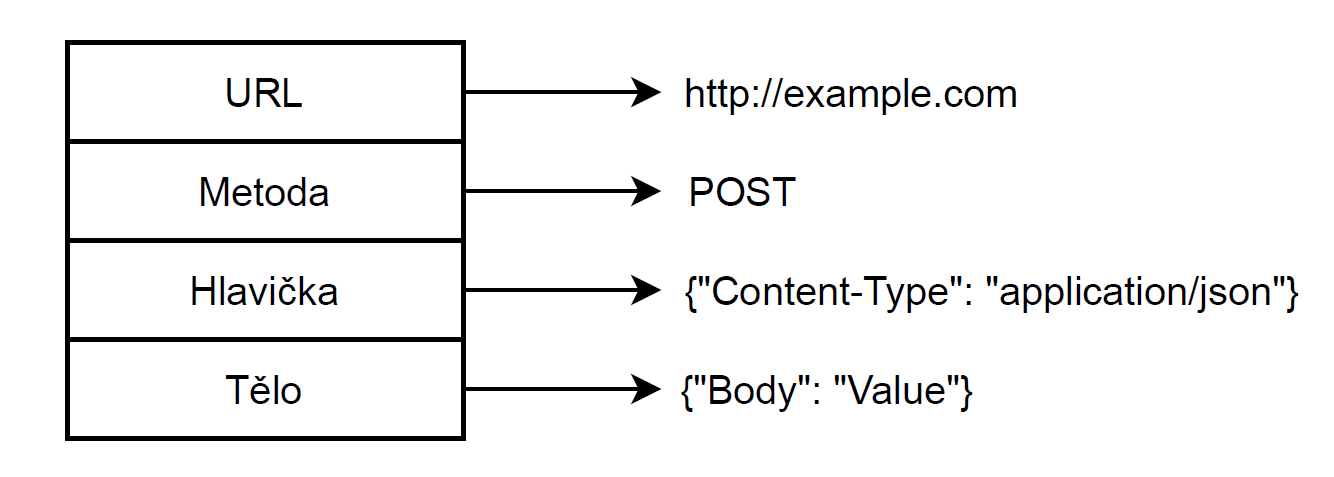
\includegraphics[width=0.9\textwidth]{obrazky-figures/HTTPstructure2.png}
	\caption{Struktura HTTP požadavku}
	\label{fig_StrukturaHTTPPozadavku}
\end{figure}

Mimo to je uvažováno, že výsledná testovací sada může být složena z testovacích případů, které nemusejí obsahovat pouze jeden HTTP požadavek, ale celou sekvenci požadavků. Příkladem jednoho takového testovacího případu může být test složený z požadavků pro vytvoření uživatele, získání všech informací a následně jeho smazání. Na tomto fiktivním příkladu si vysvětlíme, na jakých úrovních je v nástroji Suiter možné kombinace provádět. Uvažujme, že každý takový testovací případ je složen z požadavků se stejnou strukturu jako následující HTTP dotazy. Místa, kde se má parametr nahradit kombinovanou hodnotu, jsou označeny ve složených závorkách, množiny jejich hodnoty zobrazeny v tabulce \ref{table_MnozinaHodnot}.

\begin{table}[h]
\centering
\begin{tabular}{ |c||c| } 
 \hline
Parametr & Množina hodnot \\ 
 \hline
 \hline
\texttt{id} & $[123,124,125,126]$ \\
 \hline
\texttt{name} & [Martin, Pavel] \\ 
 \hline
\texttt{age} & $[20,21]$ \\
 \hline
\end{tabular}
\caption{Množina hodnot kombinovaných parametrů}
\label{table_MnozinaHodnot}
\end{table}

\begin{lstlisting}[frame=single]
POST http://example.com/api/v1/user?UserId={id} HTTP/1.1
Content-Type: application/json

{"name": {name} , "age": {age} }
\end{lstlisting}

\begin{lstlisting}[frame=single]
GET http://example.com/api/v1/user?UserId={id} HTTP/1.1

\end{lstlisting}

\begin{lstlisting}[frame=single]
DELETE http://example.com/api/v1/user?UserId={id} HTTP/1.1

\end{lstlisting}

\subsubsection*{Kombinování na úrovni části požadavku}
Prvním místem, kde může ke kombinacím docházet, je uvnitř libovolné části libovolného HTTP požadavku. Každá část HTTP požadavku může nést jisté informace, která uživatel může chtít parametrizovat a kombinovat pouze uvnitř dané části. Jinými slovy, uživatel nechce parametry jedné části kombinovat s parametry části jiné. V takovém případě je nástroji specifikované dané kritérium, které má být pro tyto lokální parametry splněno a kombinace je provedena pouze v tomto místě.

Kombinování parametrů na této úrovni je podmíněno množstvím parametrů uvnitř dané části. Kombinování je možné pouze v případě, kdy v ní jsou obsaženy alespoň dva parametry. 

Ve výše zmíněném příkladu je tak kombinace na této úrovni možná pouze pro tělo požadavku pro vytvoření uživatele, tedy požadavek s HTTP metodou POST. V těle tohoto požadavku může dojít ke kombinaci jména a věku uživatele, izolované od ostatních částí HTTP požadavku. Tato kombinace pro kritérium pokrytí dvojic je popsána v následující tabulce:

\begin{table}[h]
\centering
\begin{tabular}{ |c| } 
 \hline
\{"name": \textcolor{red}{Martin}, "age": \textcolor{red}{20} \} \\
 \hline
\{"name": \textcolor{red}{Pavel}, "age": \textcolor{red}{20} \} \\
 \hline
\{"name": \textcolor{red}{Martin}, "age": \textcolor{red}{21} \} \\ 
 \hline
\{"name": \textcolor{red}{Pavel}, "age": \textcolor{red}{21} \} \\
 \hline
\end{tabular}
\caption{Výsledné kombinace těla požadavku pro uvažovaný příklad}
\label{table_Exampleeeee}
\end{table}



Kombinováním na této úrovni může vzniknout situace, kdy některé části budou mít již přidělené kombinace hodnot, ale ostatní části nikoliv. K jejich přidělování tak bude docházet až o úroveň výše, na úrovni celého požadavku. 



\subsubsection*{Kombinování na úrovni jednoho požadavku}

Druhou úrovní, na které je možné provádět kombinace, je na úrovni celého požadavku. K této kombinaci dochází v každém požadavku bez ohledu na to, kolik parametrů je v požadavku obsaženo. Výsledný požadavek testovacího případu je zkrátka vždy tvořen kombinací URL, metody, hlavičky a jeho těla. T-Wise kritérium je tak v tomto případě rozšířeno i pro případ, kdy k žádné kombinaci reálně nedochází a je potřeba pokrýt pouze všechny hodnoty z každé množiny hodnot, tedy pokrýt toto kritérium pro $T=1$. 

Jak bylo nastíněno u předchozí úrovně, může nastat situace, kdy je potřeba kombinovat jednotlivé části, u kterých již byly přiděleny hodnoty parametrů s částmi, kde jsou hodnoty parametrů stále předmětem budoucí kombinace. Tuto situaci si demonstrujeme opět na ukázce požadavku POST, s jeho již zkombinovanými parametry těla zprávy, popsaných tabulkou \ref{table_Exampleeeee}. Na této úrovni je tedy potřeba kombinovat následující: 

% V rámci kombinací tohoto požadavku na této úrovni je potřeba kombinovat následující části:
% pak kombinujeme následující:
\begin{center}
\begin{tabular}{c}
\begin{lstlisting}[language=Python]
# URL
URL = "http://example.com/api/v1/user?UserId={id}"
URL.id = [123,124,125,126]
# Method
method = ["POST"]
# Header
header = [{"Content-Type": "application/json"}]
# Body
body = [
	{"name": "Martin", "age": 20 },
	{"name": "Martin", "age": 21 },
	{"name": "Pavel", "age": 20 },
	{"name": "Pavel", "age": 21 }
]
\end{lstlisting}
\end{tabular}
\end{center}

Všimněme si, že v tomto příkladě jediná proměnná, která stále nemá přidělenou hodnotu, je identifikátor uživatele obsažený v URL adrese. Mimo to, dvě části požadavku, metoda a hlavička, mají pouze jednu hodnotu, která bude použita ve všech testovacích případech této úrovně. Zbývají tedy pouze dvě části, které již obsahují, případně budou obsahovat víceprvkovou množinu hodnot. Tyto množiny jsou poté kombinovány způsobem popsaný v tabulce \ref{table_Exampleeeee2} pro $T=1$. 

\begin{table}[h]
\centering
\begin{tabular}{ |c|c| } 
 \hline
URL & http://example.com/api/v1/user?UserId=\textcolor{red}{123} \\
metoda & POST \\
hlavička & \{"Content-Type": "application/json"\} \\
tělo & \{"name": "\textcolor{red}{Martin}", "age": \textcolor{red}{20} \} \\ 
 \hline
URL & http://example.com/api/v1/user?UserId=\textcolor{red}{124} \\
metoda & POST \\
hlavička & \{"Content-Type": "application/json"\} \\
tělo & \{"name": "\textcolor{red}{Martin}", "age": \textcolor{red}{21} \} \\ 
 \hline
URL & http://example.com/api/v1/user?UserId=\textcolor{red}{125} \\
metoda & POST \\
hlavička & \{"Content-Type": "application/json"\} \\
tělo & \{"name": "\textcolor{red}{Pavel}", "age": \textcolor{red}{20} \} \\ 
 \hline
URL & http://example.com/api/v1/user?UserId=\textcolor{red}{126} \\
metoda & POST \\
hlavička & \{"Content-Type": "application/json"\} \\
tělo & \{"name": "\textcolor{red}{Pavel}", "age": \textcolor{red}{21} \} \\ 
 \hline
\end{tabular}
\caption{Výsledné kombinace těla požadavku pro uvažovaný příklad}
\label{table_Exampleeeee2}
\end{table}

Maximální násobnost kombinací na této úrovni je dána součtem všech parametrů bez přiřazené hodnoty a počtem víceprvkových množin s již zkombinovanými hodnotami. V případě, že by URL adresa obsahovala v našem příkladě kromě identifikátoru \textit{id} i jiný parametr, T-Wise kritérium by mohlo pokrývat až kombinace trojic. 



\subsubsection*{Kombinování na úrovni všech požadavků}

Ke kombinování na nejvyšší úrovni dochází v nástroji Suiter napříč všemi požadavky testovacího případu. To znamená, že předchozí dvě úrovně definují určité množiny variant, jakých může každý požadavek v testovací sadě nabývat. Jinými slovy, každá taková množina požadavku má stejnou strukturu, ale jsou použité jiné hodnoty pro kombinované parametry.

Je zřejmé, že k tomuto kombinování může docházet pouze v případě, kdy je testovací případ složen z více než jednoho požadavku. V opačném případě na této úrovni není co kombinovat a ve výsledné testovací sadě se tak objeví jeden testovací případ pro každou variantu tohoto požadavku.

Požadavky však nemusejí nutně obsahovat více variant, ale mohou obsahovat pouze jeden případ, který bude použit stejným způsobem v celé testovací sadě. I přesto, že každá množina požadavků může být různě velká, výslednou kombinací vznikne sada testů, kde v každém testovacím případu je použita sekvence všech zadaných požadavků.
 % vždycky jednotný počet testů, kde v každém testu jsou všechny požadavky použity a žádná není vynechána.

% Podobně jako v předchozí úrovni, i tady je možné kombinace provádět způsobem, kdy každá varianta požadavku bude použita minimálně jednou. 
Na rozdíl od předchozí úrovně tak nemůže dojít k situaci, kdy některá hodnota parametru uvnitř požadavku nebyla nakombinována. Všechny požadavky již mají jasně specifikované parametry a dochází tedy ke kombinacím pouze kompletních množin. Maximální násobnost kombinací T je definovaná součtem všech víceprvkových množin. 

Uvažujme, že v našem příkladu došlo na předchozích úrovních k následujícím kombinacím, popsaných tabulkou \ref{table_KombinaceTretiUroven}. Pro jednoduchost jsou zobrazeny pouze kombinace parametrů bez specifikace celé struktury požadavku. Jednotlivé sloupce popisují tři požadavky POST, GET a DELETE, které mají být provedeny. Každý tento požadavek je složen ze čtyř kombinací jeho parametrů. Maximální možná kombinační síla v tomto příkladě je tedy $3$. Pokrytím všech trojic by vznikla testovací sada obsahující $4*4*4=64$ testovacích případů, z nichž některé jsou zobrazeny v tabulce \ref{table_ExampleTretiUrovenVysledek}.

% , protože každý z požadavků obsahuje více než jednu kombinaci hodnot, s jakými může být tento požadavek zavolán. Pro $T=3$ tedy může vzniknout až $4*4*4=64$ variant, které samozřejmě neukážeme všechny, ale některé z nich jsou popsány tabulkou .

\begin{table}[h]
\centering
\begin{tabular}{ |c||c|c||c||c| } 
 \hline
požadavek & \multicolumn{2}{c||}{POST} & GET & DELETE \\
 \hline
 \hline
parametry & \multicolumn{2}{c||}{[id,name]} & [id] & [id] \\
 \hline
\multirow{4}{*}{kombinace} & \multicolumn{2}{c||}{[123,Martin]} & [123] & [123] \\
& \multicolumn{2}{c||}{[124,Martin]} & [124] & [124] \\
& \multicolumn{2}{c||}{[125,Pavel]}  & [125] & [125] \\
& \multicolumn{2}{c||}{[126,Pavel]}& [126] & [126] \\
 \hline
\end{tabular}
\caption{Přehled kombinací pro náš příklad splňující kritérium pair-wise}
\label{table_KombinaceTretiUroven}
\end{table}
\begin{table}[h]
\centering
\begin{tabular}{ |c||c|c||c||c| } 
 \hline
 & \multicolumn{2}{c||}{POST} & GET & DELETE \\
 \hline
 \hline
 Test Case ID & \multicolumn{2}{c||}{[id,name]} & [id] & [id] \\
 \hline
1 & \multicolumn{2}{c||}{[123,Martin]} & 123 & 123 \\
2 & \multicolumn{2}{c||}{[123,Martin]} & 123 & 124 \\
3 & \multicolumn{2}{c||}{[123,Martin]} & 123 & 125 \\
... & \multicolumn{2}{c||}{...} & ... & ... \\
64 & \multicolumn{2}{c||}{[126,Pavel]} & 126 & 126 \\
 \hline
\end{tabular}
\caption{Přehled kombinací pro náš příklad splňující kritérium pair-wise}
\label{table_ExampleTretiUrovenVysledek}
\end{table}

Intuitivně však dává větší smysl, aby identifikátor \textit{id}, byl použit ve všech testovacích případech se stejnou hodnotou. K tomuto účelu se v nástroji Suiter používají globální proměnné popsané v následující sekci.


\subsection*{Specifikace parametrů}
\label{subsec_SpecifikaceParam}

Jak již bylo v předchozí sekci ukázáno, v některých případech uživatel může mít potřebu nekombinovat všechny parametry zvlášť, ale nastavit některému parametru jistou závislost na jiném parametru. Tato závislost zajišťuje, že dané parametry budou mít napříč celým testovacím případem stejnou hodnotu. 

Obecně se tak parametry, použité k označení kombinovaných hodnot, mohou rozdělit na dva typy: \textit{lokální} a \textit{globální}. Lokální parametry mají tu vlastnost, že jejich hodnota je použita pouze v místě její kombinace a není ukládaná pro pozdější využití. Oproti tomu globální parametry jsou kombinovány na místě jeho prvního výskytu a v případě, že implementovaný algoritmus, popsaný v kapitole \ref{ch_ImplementaceSuiter}, narazí na globální parametr se stejným identifikátorem, použije jemu odpovídající hodnotu i na tomto místě.  

 % Hodnota těchto proměnných je kombinována pouze na místě jeho prvního výskytu a v případě, že implementovaný algoritmus, popsaný v kapitole \ref{ch_ImplementaceSuiter}, narazí na globální parametr se stejným identifikátorem, použije jemu odpovídající hodnotu.

Jak lokální, tak globální parametry je možné použít na všech kombinačních úrovních. Nastává však otázka, jakým způsobem by měly být tyto parametry označeny, a především jakým způsobem by měl být předán kontext globálních proměnných napříč všemi úrovněmi. 

Každý kombinovaný parametr je v jeho vstupní hodnotě označen pomocí sekvence znaků definující začátek a konec parametru. K tomu, aby bylo možné odlišit lokální a globální parametry jsou pak použity odlišné sekvence. Zahajovací a ukončovací znaky však nejsou jasně definovány jednou konkrétní hodnotou. Uživatel si tak dle potřeby může sám zvolit, jaké sekvence znaků jsou v jeho případě unikátní. Tyto hodnoty jsou zadány v konfiguračním souboru, jehož příklad je k nahlédnutí v příloze \ref{chap_ConfigFile}. 





\section{Architektura nástroje}
\label{sec_ArchitekturaNastroje}

V této sekci je objasněna struktura nástroje Suiter. Cílem je vytvořit procedurální aplikaci, jejíž základní funkcionalita je zobrazena sekvenčním diagramem \ref{fig_SequenceDiagram}. Diagram popisuje vzájemnou komunikaci nejdůležitějších modulů, ze kterých je aplikace složena.

\begin{figure}[hbt]
	\centering
	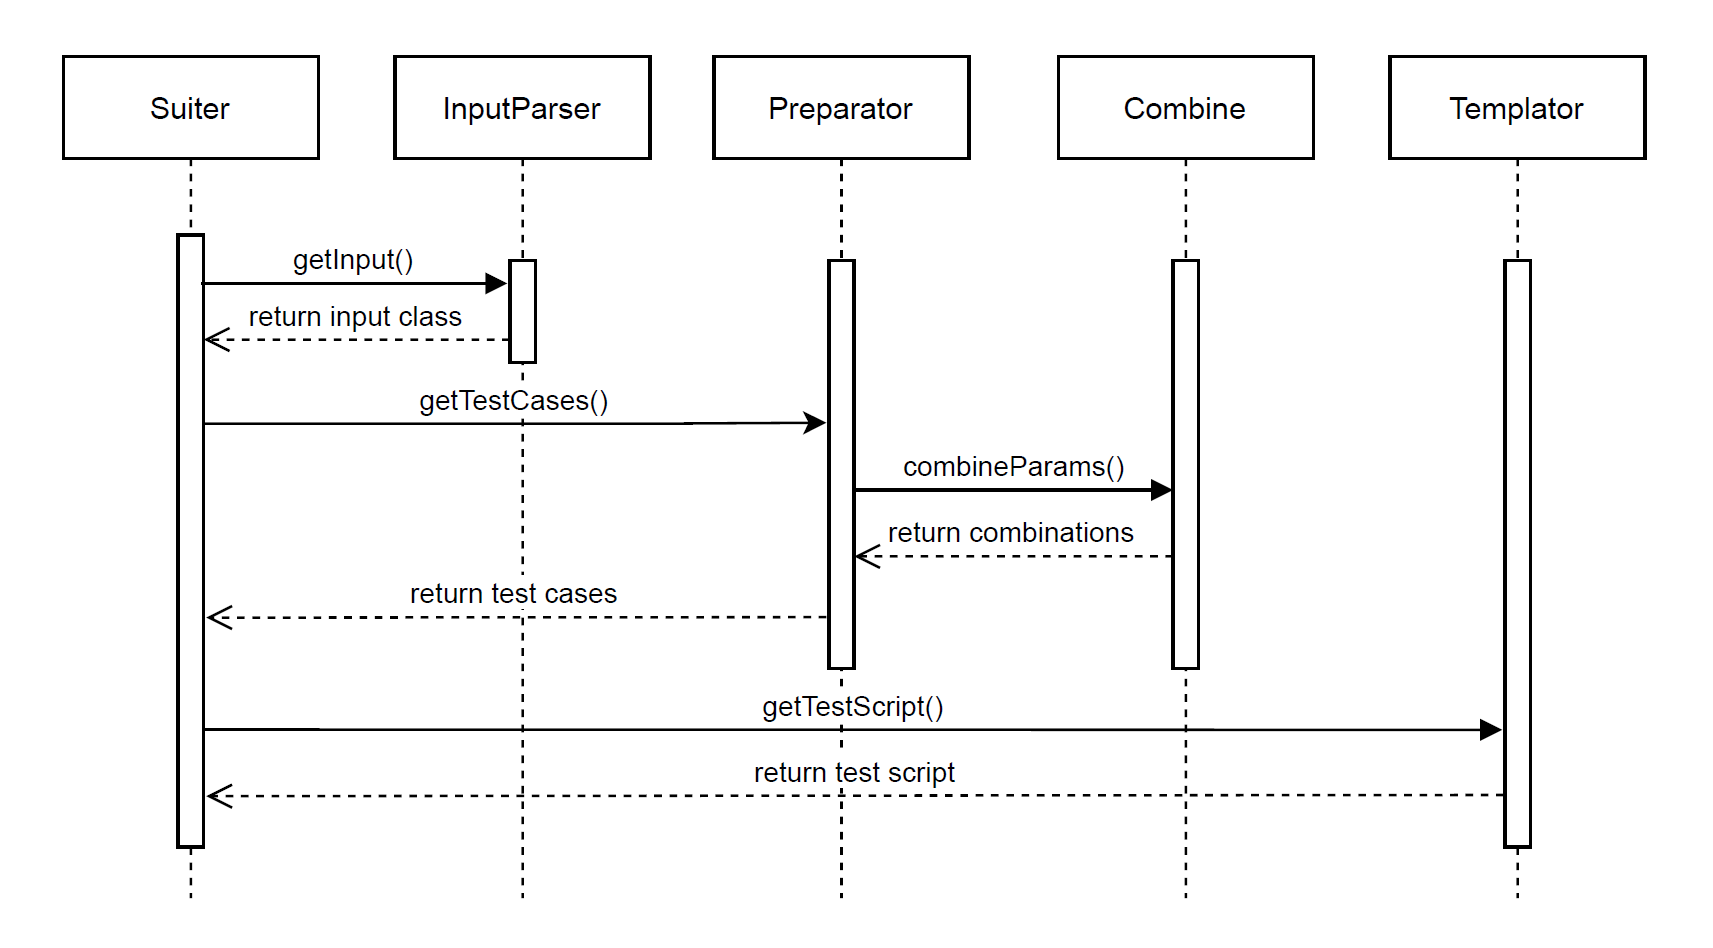
\includegraphics[width=1\textwidth]{obrazky-figures/SequenceDiagram2.png}
	\caption{Sekvenční diagram popisující základní funkcionalitu nástroje Suiter}
	\label{fig_SequenceDiagram}
\end{figure}

Vstupní bod tohoto nástroje je definován v modulu nazvaném \textit{Suiter}. Zde se nachází hlavní sekvence příkazů, využívající funkcionalitu ostatních modulů. Na základě vstupního a konfiguračního souboru jsou vytvořeny třídy obsahující informace o požadavcích na výslednou testovací sadu. S ohledem na tyto požadavky je volán modul \textit{Preparator}, který s využitím nástroje \textit{Combine}, popsaného v \ref{subsec_Combine}, připravuje a vytváří jednotlivé testovací případy, které mají být v sadě obsaženy. Posledním modulem je \textit{Preparator}, který vytváří výsledný testovací skript vygenerovaný pro požadovaný programovací jazyk.
% který na základě frameworku testovacího skriptu tento skript vytvoří.


% Tento diagram popisuje komunikaci základních modulů, jenž budou podrobněji popsány dále v této kapitole.
Přestože aplikace bude implementována procedurálně, jsou v aplikaci využity jisté prvky objektově orientovaného programování. Ty spočívají především v použití tříd pro reprezentaci vstupních dat uživatele a pro reprezentaci dat obsažených v konfiguračním souboru. Oba tyto uživatelské vstupy jsou převedeny do tříd \textit{InputData} a \textit{ConfigData}, popsaných pomocí diagramu tříd \ref{fig_DiagramTridInput} a \ref{fig_DiagramTridConfig}. Nad těmito třídami není umožněno provádět prakticky žádné operace a slouží tedy čistě pro jednotnou reprezentaci vstupních dat.

Třída reprezentující vstupní data obsahuje informace o množinách hodnot všech globálních parametrů a je dále složena z objektů, představující jednotlivé HTTP požadavky, které se mají v sekvenci provést. Každý třída HTTP požadavku je rozložena do 4 dalších tříd, nesoucí informace o jeho hodnotě, síle kombinačního kritéria a množině hodnot všech lokálních parametrů. Třída reprezentující hlavičku a tělo HTTP požadavku navíc může obsahovat i cestu k souboru, jelikož hodnoty těchto částí nemusejí být v aplikaci Suiter specifikovány konkrétní hodnotu, ale i obsahem souboru.

\begin{figure}[hbt]
	\centering
	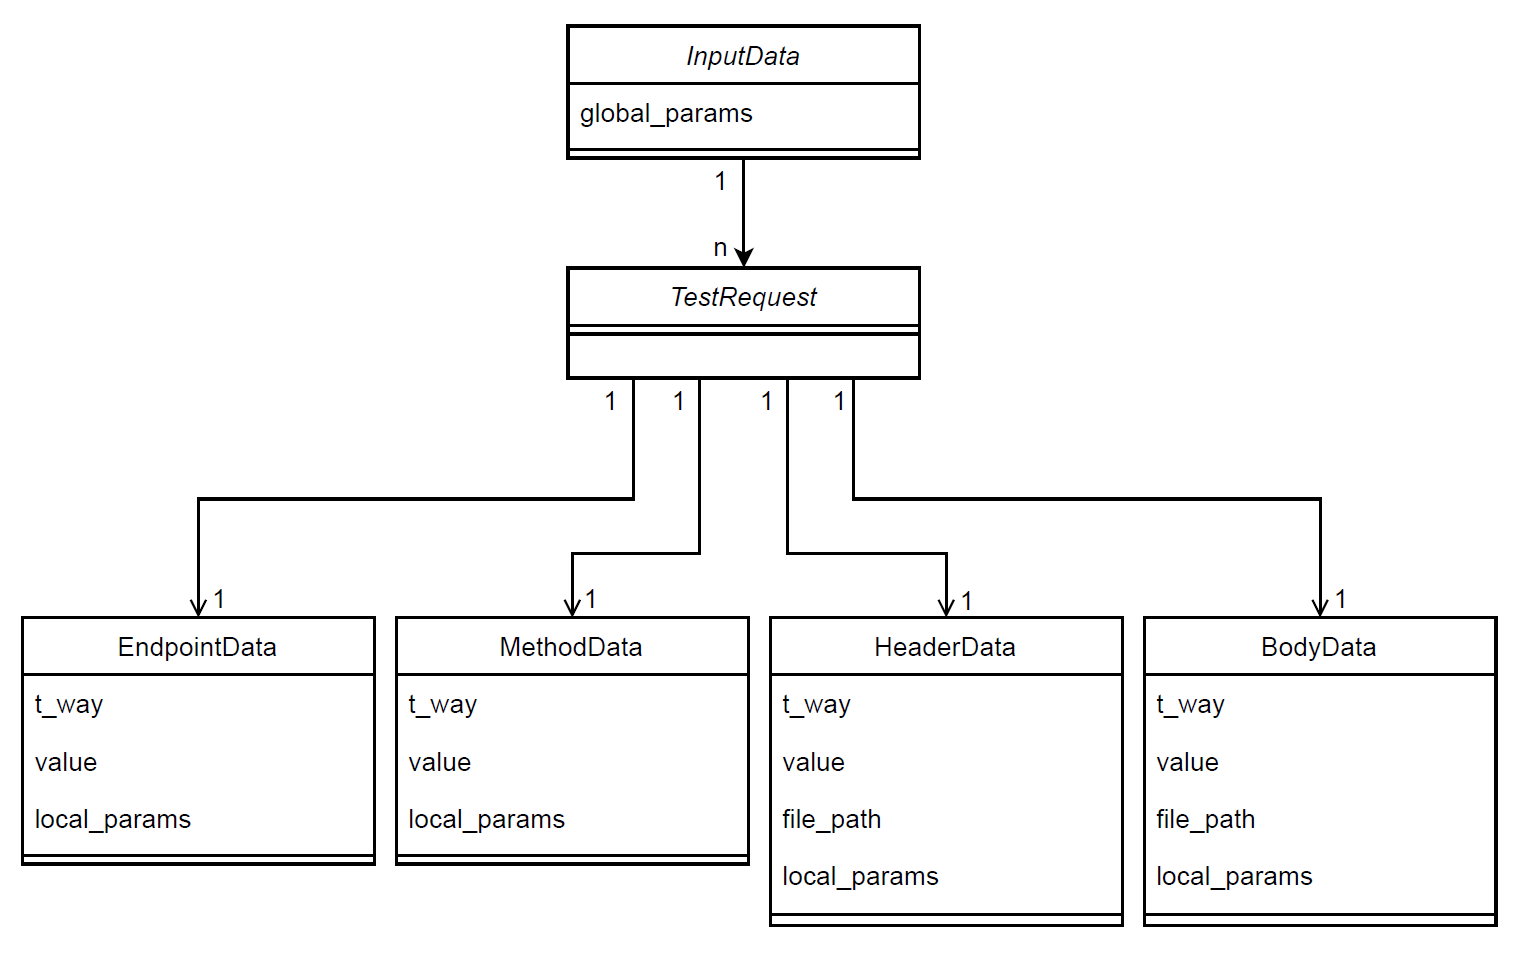
\includegraphics[width=1\textwidth]{obrazky-figures/InputClass3.png}
	\caption{Diagram tříd popisující reprezentaci vstupních dat nástroje Suiter}
	\label{fig_DiagramTridInput}
\end{figure}

 % každá pro obsahuje objekt pro každou část
 % definujícího sekvenci jednotlivých požadavky

% , které mají být v rámci jednoho testovacího dalších čtyř tříd, nesoucích informace o jednotlivých částech HTTP požadavku. Každá tato část může obsahovat například informace o síle kombinačního kritéria, které má být v rámci dané části provedeno, množina hodnot lokálních parametrů.
% Těmito inforamcemi je například hodnota tohoto stringu

Třída reprezentující data konfiguračního souboru je založená na podobném principu. V první třídě jsou specifikovány atributy nesoucí informace o cestě ke vstupnímu souboru, složce určené pro výstup nástroje Suiter, limitní hodnotě definující maximální počet testovacích případů a také informace o frameworku, který má být použit pro výsledné testovací skripty. Tato třída poté obsahuje hierarchickou strukturu dalších tříd, pomocí kterých jsou definovány znaky určující začátek a konec lokálních a globálních parametrů pro každou část HTTP požadavku. 

% , cestě ke vstupnímu souboru, složce určené pro výstup nástroje Suiter a v také specifikaci maximálního množství testovacích případů, které mohou být nástrojem vygenerovány.

% složce, do které bude výsledný testovací skript vložen společně s pomocnými soubory jako obsah hlaviček a těl pro všechny testovací případy.
\begin{figure}[hbt]
	\centering
	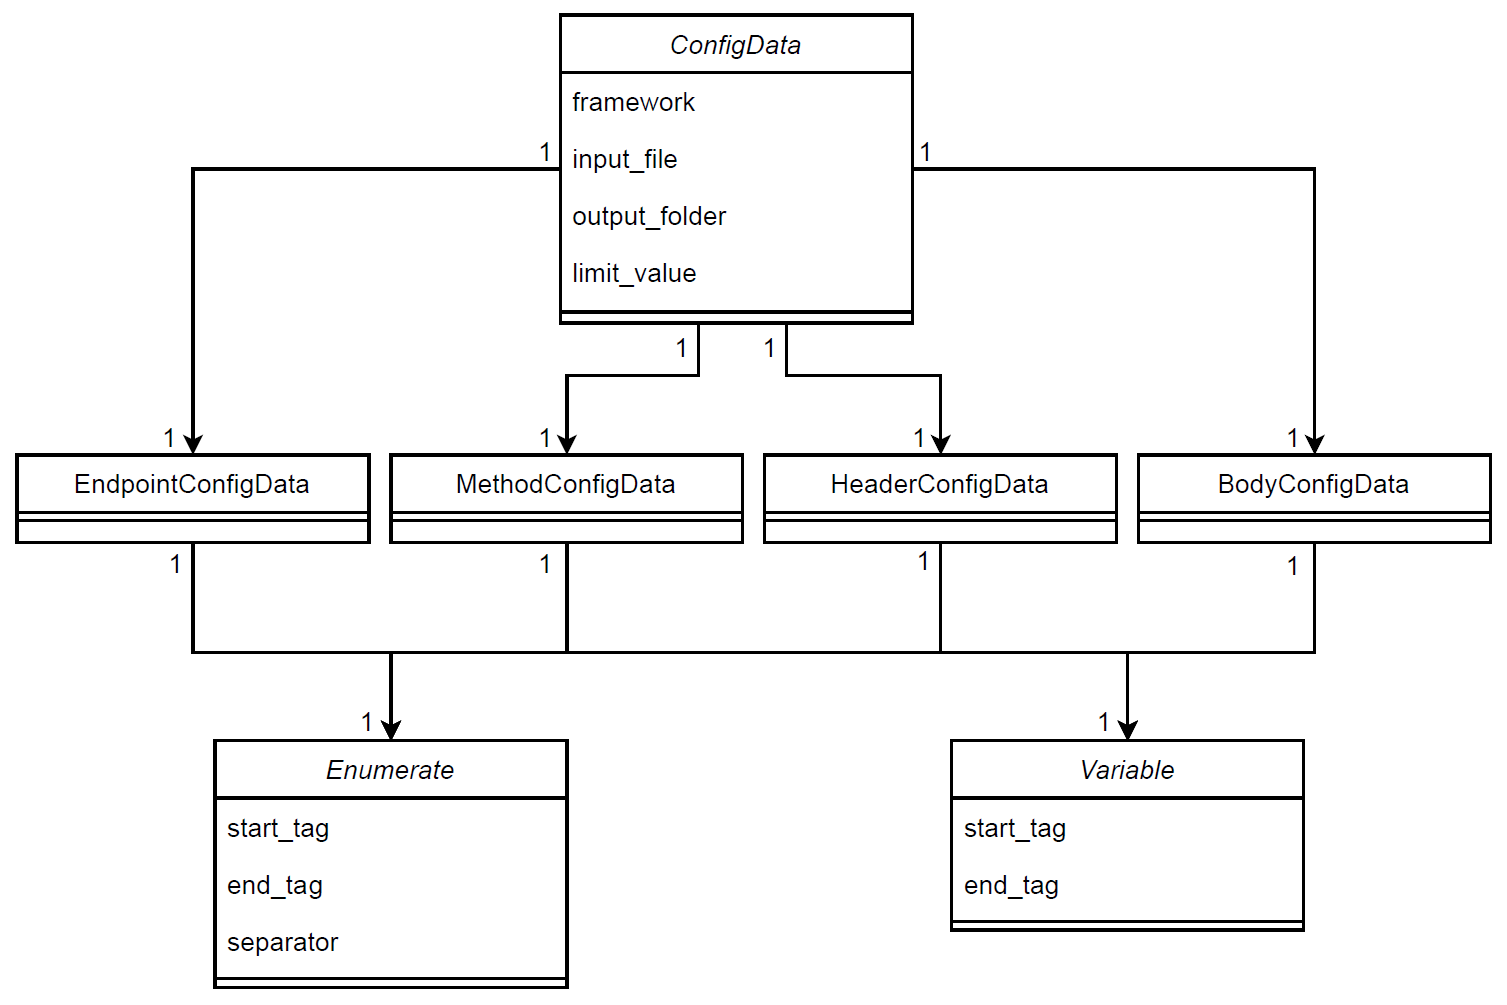
\includegraphics[width=1\textwidth]{obrazky-figures/testClassDiagram3.png}
	\caption{Diagram tříd popisující reprezentaci konfiguračních dat nástroje Suiter}
	\label{fig_DiagramTridConfig}
\end{figure}





% Pro kombinace těchto vstupních parametrů je použito kritérium T-Wise, popsané v \ref{subsec_twc}. Parametry jendotlivých volání se kombinují několika úrovních. Uživatel pak specifikuje sílu kombinací pro každou tuto úroveň,případně nespecifikuej a bude pouzita defaultni.

% V této kapitole si popíšeme návrh a implementaci konzolové aplikace Suiter. Aplikace slouží pro generování spustitelné testovací sady na základě kombinování vstupních parametrů webových služeb, komunikující protokolem HTTP. Důraz je kladen na testování webových služeb podporující architekturu REST, nicméně se dá použít i pro testování komunikace v jakékoliv jiné aplikaci využívající protokol HTTP.
% jakoukoliv jinou komunikaci využívající prtokol HTTP.

\chapter{Implementace nástroje Suiter} 
\label{ch_ImplementaceSuiter}

Tato kapitola shrnuje postup implementace nástroje Suiter, generující spustitelné testovací skripty jazyka Python a JavaScript. Jak bylo ukázáno v sekci \ref{sec_ArchitekturaNastroje}, popisující navrhnutou architekturu, aplikace se skládá z modulů, jejichž implementace je provedena imperativním způsobem programování s využitím tříd pro reprezentaci vstupních dat uživatele.
% napsaných pomocí programovacího jazyka Python. 

% Nástroj je implementovaný s využitím programovacího jazyka Python procedurálním stylem s využitím prvků OOP, tříd. Tyto třídy jsou použity pouze pro reprezentaci vstupních dat vstupního souboru a konfiguračního souboru. 

V první části této kapitoly jsou shrnuty technologie, které jsou použity pro jeho implementaci. V navazujících částech jsou poté popsány způsoby implementace jednotlivých částí programu. Zaměření je kladeno na popis vstupního rozhraní, způsobu kombinování jednotlivých parametrů mezi sebou a je zde popsána i komunikace s nástrojem Combine, který je pro účely tohoto kombinování použit. Další sekce se zabývá popisem výsledných testovacích sad a jejich vkládání do testovacích skriptů. Testování nástroje Suiter je následně popsáno na konci této kapitoly.

% Implementace probíhala iterativně a v průběhu se značně lišila, jak použitými technologiemi, tak i celkovou strukturou aplikace. Bude zde tedy popsána pouze finální implementace patřičných částí. V průběhu času se značně měnila.

\section{Použité technologie}
\label{sec_Technologie}

Tato sekce se zabývá popisem technologií, které byly v rámci práce použity. Nástroj Suiter je implementovaný využitím programovacího jazyka Python. Pro výsledné testovací skripty a testování samotného nástroje je použita kombinace technologií Pytest, Mocha a Flask. Pytest a Mocha pro tvorbu a spouštění testů, Flask pak pro vytvoření webové služby, která bude v rámci této práce představovat testovaný systém. V neposlední řadě je potřeba zmínit aplikaci Combine, která je využita pro tvorbu kombinací dle potřebného kritéria. 

% Jedná se pouze o popis daným technologií.

\subsection*{Python}
Python\footnote{https://www.python.org/} je interpretovaný vysokoúrovňový programovací jazyk, který je velmi atraktivní zejména pro aplikace, které vyžadují rychlé prototypování. Díky podpoře různých programovacích paradigmat je velmi univerzální. Pomocí Pythonu lze vytvářet aplikace jak čistě procedurální, tak čistě objektové. Případně je možné využít kombinace obou paradigmat. Mimo to Python využívá moduly a balíčky, podporující modularitu programu a opětovné použití kódu. Jeho jednoduchá a snadno pochopitelná syntaxe umožňuje snadnou čitelnost, a proto snižuje náklady na údržbu programu. Jeho hlavní nevýhodou v porovnání s kompilovanými jazyky je jeho nepříliš vysoká rychlost a vysoká spotřeba paměti a skutečnost, že chyby obsažené v programu lze odhalit pouze za běhu programu. Interpret Pythonu a jeho rozsáhlé množství balíčků je dostupný zdarma na všechny standardní platformy a lze jej volně distribuovat. 
% Mimo to podporuje dynamickou kontrolu datových typů a díky podpoře různých programovacích paradigmat je velmi univerzální. 
% Nástroj Suiter je implementovaný pomocí vysokoúrovňového skriptovacího programovacího jazyka Python, který usnadnil práci mnohými užitečnými knihovnami. Jednou z nich je například knihovna \textit{configparser}
% Aplikace je napsaná pomocí programovacího jazyka Python s využitím jeho knihoven. Pro testovací prostředí, která představuje aplikaci, na kterou se budou posílat požadavky, je napsaná pomocí framewroku Flask. Jedná se o framework, který slouží k vytváření webových aplikací. V případě našeho testovacího prostřední bude však webová aplikace pracovat pouze na našem lokálním prostředí a na síti vůbec nebude.

\subsection*{Flask}
\label{subsec_Flask}
Flask\footnote{https://flask.palletsprojects.com/} je framework, napsaný v jazyce Python, sloužící k tvorbě webových aplikací. Flask v porovnání s ostatními frameworky spoléhá na jeho jednoduché jádro, které je snadno rozšiřitelné. Flask tak nechává většinu rozhodnutí na uživateli a v základu neobsahuje rozhraní pro komunikaci s databází, ověřování webových formulářů ani jednotný způsob autentizace. Uživatel si tak sám určí, co přesně od dané aplikace vyžaduje. 


\subsection*{Combine}
\label{subsec_Combine}
Combine\footnote{https://combine.testos.org/} je webový nástroj, který umožňuje testerům vytvořit testovací sadu uspokojující dané T-Wise kritérium. Nabízí možnost specifikovat parametry 10 datových typů, pro představu například celá a desetinná čísla, textové řetězce, či případně datové typy enum, které umožňují výčtem specifikovat libovolnou hodnotu kombinovaného parametru, a pomocí kterého je možné kombinovat například i objekty. Combine podporuje tvorbu testovacích sad splňující T-wise kritérium až pro šestice, tedy pro $T=6$. Mimo to umožňuje pomocí dodatečných informací vyloučit z výsledné testovací sady určité kombinace bloků, které jsou neplatné, případně nemohou nikdy nastat. Nástroj je dostupný v rámci platformy Testos a byl vytvořen v bakalářské práce Radima Červinky \cite{1_Combine}.



\subsection*{Pytest}
Pytest\footnote{https://docs.pytest.org/} je testovací framework, který usnadňuje vytváření testovacích skriptů pomocí programovacího jazyka Python. Pytest pomáhá tvořit jednoduché, dobře škálovatelné a čitelné testy pro databáze, uživatelské rozhraní a velmi často právě pro API. 


\subsection*{Node.js a Mocha}
Node.js\footnote{https://nodejs.org/} je asynchronní běhové prostředí řízené událostmi, které umožňuje spouštět kód skriptovacího jazyka JavaScript mimo webový prohlížeč. Je určený pro psaní vysoce škálovatelných internetových aplikací, především webových serverů, nicméně má i mnoho jiných využití. Příkladem je testovací framework Mocha, který funguje právě na tomto prostředí.

% https://blog.logrocket.com/a-quick-and-complete-guide-to-mocha-testing-d0e0ea09f09d/#whatismochajs
Mocha \footnote{https://mochajs.org/} je volně dostupná testovací knihovna, běžící jak v Node.js, tak v prostředí prohlížeče. Je určena pro testování jak synchronních, tak asynchronních aplikací s velmi uživatelsky přívětivým uživatelským rozhraním. Mocha testy probíhají sériově, což umožňuje flexibilní a přesné reportování jednotlivých testovacích případů. 

% s přesným mapováním výjimek ke správným testovacím případům.

% Podporuje browser support, asynchronous testing, test coverage reports, and use of any assertion library. Je určen především pro asynchronní testování a dělá ho jendoduché. Mocha testy běží sériově, umožňují flexibilní a přesné reportování

% Programy pro Node.js jsou psané v jazyce JavaScript, hojně využívající model událostí a asynchronní operace pro minimalizaci režie procesoru a maximalizaci výkonu.





\section{Implementace vstupního rozhraní}
\label{sec_VstupniRozhrani}

Vstupní rozhraní nástroje Suiter je rozděleno do tří částí, kterými uživatel ovlivňuje jeho chování. Jelikož se jedná o konzolovou aplikaci, uživatel může část chování ovlivnit pomocí argumentů při jeho spuštění. Druhou možností je specifikování hodnot konfiguračního souboru. Nejdůležitějším uživatelským vstupem je však soubor, pomocí kterého jsou specifikovány požadavky na výslednou testovací sadu, případně je tato sada Suiteru přímo poskytnuta.

% mu jsou předána přímo množina testovacích případů, na základě kterých je testovací skript vytvořen.

Soubor, popisující základní vstupní požadavky uživatele, může mít tedy dva formáty. Tyto formáty jsou závislé na použitých argumentech při spuštění aplikace. Při jeho běžném spuštění, je automaticky předpokládáno, že obsah předaného souboru představuje požadavky na kombinace, které mají být provedeny. Předáním vstupního souboru s argumentem \textit{'--skip'} dojde k přeskočení algoritmu kombinujícího parametry a výsledný skript je složen pouze z testovacích případů popsaných právě tímto souborem.

% Posledním a taky nejpodstatnějším uživatelským vstupem je však soubor, pomocí kterého jsou definovány požadavky na testovací případy, které mají být v testu obsaženy.
 % a specifikovat požadavky, které má výsledný testovací skript splňovat. 

\subsection*{Vstupní soubor popisující požadavky}

\definecolor{delim}{RGB}{20,105,176}
\definecolor{numb}{RGB}{106, 109, 32}
\definecolor{string}{rgb}{0.64,0.08,0.08}
\lstdefinelanguage{json2}{
    frame=single,
    rulecolor=\color{black},
    showspaces=false,
    showtabs=false,
    breaklines=true,
    postbreak=\raisebox{0ex}[0ex][0ex]{\ensuremath{\color{gray}\hookrightarrow\space}},
    breakatwhitespace=true,
    upquote=true,
    morestring=[b]",
    stringstyle=\color{string},
    literate=
     *{0}{{{\color{numb}0}}}{1}
      {1}{{{\color{numb}1}}}{1}
      {2}{{{\color{numb}2}}}{1}
      {3}{{{\color{numb}3}}}{1}
      {4}{{{\color{numb}4}}}{1}
      {5}{{{\color{numb}5}}}{1}
      {6}{{{\color{numb}6}}}{1}
      {7}{{{\color{numb}7}}}{1}
      {8}{{{\color{numb}8}}}{1}
      {9}{{{\color{numb}9}}}{1}
      {\{}{{{\color{delim}{\{}}}}{1}
      {\}}{{{\color{delim}{\}}}}}{1}
      {[}{{{\color{delim}{[}}}}{1}
      {]}{{{\color{delim}{]}}}}{1},
}

Základním vstupním souborem aplikace Suiter je soubor ve validním JSON\footnote{https://www.json.org/} formátu. Pomocí tohoto souboru jsou definovány požadavky na kombinace parametrů, které mají být na jednotlivých kombinačních úrovních splněny. Dále tento soubor definuje strukturu testovacího případu, tedy sekvenci HTTP požadavků, které se mají v každém testu provést. 
 
Struktura JSON souboru je složena z objektu \textit{test\_sequence}, pole \textit{global\_params} a hodnoty \textit{t-way}, definující sílu kombinace pro nejvyšší kombinační úroveň. V objektu \textit{test\_sequence} je definovaná sekvence požadavků, které mají být v testovacím případů provedeny, včetně struktury každého HTTP požadavku. Pole \textit{global\_params} pak určuje množiny hodnot globálních parametrů použité v této sekvenci.

\begin{lstlisting}[language={json2}]
{
	"test_sequence": [
		{
			"endpoint": {...},
			"method": {...},
			"header": {...},
			"body": {...},
			"t-way": 2
		},
		{
			"endpoint": {...},
			"method": {...},
			"header": {...},
			"body": {...},
			"t-way": 3
		}
	],
	"t-way": 2,
	"global_params": {...}
}
\end{lstlisting}

Každý testovací případ v sekvenci je složený z objektů popisujících jednotlivé části HTTP požadavku, včetně specifikování případných množin lokálních parametrů a síle kombinačního kritéria \textit{t-way}. Na následujícím příkladu je zobrazena ukázka URL adresy obsahující jeden parametr, označený znaky \texttt{'<>'}.

\begin{lstlisting}[language={json2}]
"endpoint": {
	"values": "http://example.com/api/v1/user?<>,
	"local_params": [
		{ "values": [1,2,3] }
	]
}
\end{lstlisting}


% Testovací sekvence je složena z objektů definující jednotlivé části. V každé úrovni pak uživatel specifikuje zadáním parametru \textit{t-way} 
% částí, hodnot, klíčů, které jsou na nejvyšší úrovni zobrazeny, předány. Jedná se o sekvenci požadavků, které se mají v každém testu provést, kombinační kritérium na nejvyšší úrovni, tedy na provni kombinování všech požadavků mezi seboua množiny globálních parametrů, které jsou v nějakých částech nějakého HTTP požadavku obsaženy.

% Každý požadavek v sekvenci všech požadavků testovacího případu je složen z následující struktury. Obsahuje tedy informace o hodnotě, jakou daný string nabývá, včetně označených parametrů. Způsob, jakým jsou tyto paraemtry označeny včetně způsobu, jakým je předán kontext globálních parametrů napříč všemi úrovněmi kombinaci, je vysvětlen v sekci X.
%  a případné síle kombinačního kritéria

Parametry se mohou vyskytovat v každé části HTTP požadavku. A to jak lokální, tak globální. Dokonce mohou být obsaženy i uvnitř souboru. Z tohoto důvodu je pro každou hlavičku a tělo umožněno specifikovat jejich hodnotu cestou k tomuto souboru. V takovém případě může vypadat struktura specifikace následovně: 

\begin{lstlisting}[language={json2}]
"body": {
	"file_path": "../body_file.yaml",
	"local_params": [
		{ "values": ["paramInFile_X", "paramInFile_Y"] },
		{ "values": [123, 456] },
		{ "values": [True, False] }
	],
	"t-way": 2
},
\end{lstlisting}

Ukázka, jakým způsobem může vypadat vstupní soubor pro sady, kde testovací případy jsou složeny z jednoho HTTP požadavku, je zobrazena v příloze \ref{chap_VstupAplikace}.

% Kazda  cast dale muze obsahovat t-way, ktery urcuje, jestli se maji hodnoty uvnitr teto casti kombnovat ci nikoli. Soucasne urcuje, s jakou silou pak kombinovany budou. Sila nesmi presahovat pocet parametru uvnitr techto casti, stejne tak jako pocet lokalnich parametru musi presne odpovidat poctu oznacenych paraemtru.

% Parametry se mohou vyskytovat v kazde z techto uvedenych casti, kazda muze byz parametrizovana. Soucasne v priapde, ze se je header nebo soubor predan jako cesta k souboru a ne primo jeho hondtnotu, stringu, pak se parametry vyhledavaji i uvnitr tohoto souboru.



% \begin{lstlisting}[language={json2}]
% "endpoint": {
% 	"values": "http://127.0.0.1:5000/api/v1/calculator",
%     "local_params": []
% },
% "method": {
% 	"values": "<>",
% 	"local_params": []
% },
% "header": {
% 	"values": {"Content-type": "json"},
% 	"local_params": [
% 		{
% 			"values": ["header.yaml"]
% 		}
% 	],
% 	"param_is_in_file": false
% },
% "body": {
% 	"values": "",
% 	"files": "",
% 	"local_params": []
% }
% \end{lstlisting}

 % je navíc možné nástroji předat již existující nakombinované testovací případy, pro které Suiter pouze vytvoří spustitelné skripty.
% tedy bez specifikování jiného chování
% , že předaný soubor představuje soubor, jehož obsah dodržuje strukturu JSON formátu.
% Tyto formáty se odvíjí od toho, co má se vstupním souborem Suiter udělat. V případě, že závislé od toho, co má Suiter provádět za operaci.
% Vstupní soubor nástroje Suiter je specifikován v závislosti na tom, jestli mu jsou tímto souborem předány inforamce o kombinacích, které mají být provedeny, nebo je nástroji předána přímo celá již vytvořená testovací sada.

\subsection*{Vstupní soubor popisující testovací případy}
\label{subsec_VstupniSouborTestovaciPriday}

Jak bylo již zmíněno, uživatel nástroje Suiter nemusí využít funkcionality kombinující parametry, ale může specifikovat sám své vlastní testovací případy, které mají být ve výsledném testu obsaženy. Soubor určený pro tento účel má následující strukturu. Jedná se o formát, který je jednoduše převeditelný do třídimenziálního pole programovacího jazyka Python.

\begin{lstlisting}[language=Python, frame=single, basicstyle=\small]
[
	[
		[
			'http://127.0.0.1:5000/api/v1/serviceX', 
			'GET', 
			'{"Content-type": "json"}', 
			'./body_files/body1.json'
		],
		...
	],
	[
		[
			'http://127.0.0.1:5000/api/v1/serviceY', 
			'GET', 
			'{"Content-type": "yaml"}', 
			'./body_files/body2.yaml'
		],
		...
	],
	...
\end{lstlisting}

V tomto příkladě je testovací sada složena ze dvou případů, kde každý z nich obsahuje pouze jeden HTTP požadavek. Soubor může být specifikován i bez použití bílých znaků, ty byly použity pouze pro intuitivnější znázornění. V rámci zachování jednotného rozhraní má tento vstupní soubor stejnou strukturu jako výstup z modulu \textit{Preparator} zobrazeného v sekvenčním diagramu \ref{fig_SequenceDiagram}.



\section{Způsob označení parametrů}

Jak již bylo popsáno v sekci zabývající se vstupním rozhraním, v kontextu této práce existují dva typy kombinovaných parametrů - \textit{lokální} a \textit{globální}. Jejich rozdíl a základní představa o jejich způsobu využití, byla objasněna v kapitole zabývající se návrhem aplikace \ref{subsec_SpecifikaceParam}. Tato sekce je věnována překážkám, ke kterým docházelo při implementaci tohoto návrhu. A to včetně způsobu, jakým byly tyto překážky vyřešeny.

Spojením návrhu a implementace vstupního rozhraní, dochází k následujícím variantám, jakými mohou být parametry specifikovány. Demonstrace je provedena pouze na specifikování parametrů pro část HTTP požadavku, popisující její URL adresu. Ostatní části požadavku jsou však založené na totožném principu, a to včetně u označování parametrů uvnitř souboru. 
% V ostatních částech je však využito totožného principu.
\begin{lstlisting}[frame=single]
"values": "http://example.com/api/v1/user?<>,
"values": "http://example.com/api/v1/user?<1,2,3>,
"values": "http://example.com/api/v1/user?<:userId:>,
\end{lstlisting}

Na zmíněném příkladu jsou 3 způsoby zadávání parametru. První případ pouze označuje místo, kde má být použita hodnota lokálního parametru, jejíž množina hodnot je obsažena ve vstupní JSON struktuře pod klíčem \textit{local\_params}. Druhý přístup umožňuje zadávat hodnoty bez nutnosti specifikace této množiny odděleně. Posledním příklad pak zobrazuje způsob, jakým mohou být označovány globální parametry.
% mimo, zvlast, sepraratne ale jejich hodnoty jsou obsaženy přímo uvnitř identifikátoru parametru. 

Ve všech těchto ukázkách však byla použita pouze jedna výchozí hodnota pro identifikování lokálních a globálních parametrů. V případě lokálních je zahajovací znak označen symbolem \texttt{<}, ukončovací pak symbolem \texttt{>}. Předpokládá se, že tyto znaky budou v řetězci použity pouze pro označení lokálních parametrů. Musejí tedy být napříč řetězcem unikátní. To se však nemusí vždy podařit a uživatel v některých situacích může vyžadovat, aby tyto znaky bylo možné použít i v kontextu samotného řetězce. Tedy bez toho, aby je algoritmus vyhodnotil jako znaky definující nějaký parametr. Obzvláště problematické je to v těle HTTP zprávy, jelikož tělo může obsahovat sekvenci prakticky libovolných znaků. Zvolení unikátních identifikátorů pro každou část je tedy poměrně problematické, v případě těla dokonce nemožné.

Tento problém byl vyřešen použitím proměnlivých hodnot, které si uživatel může specifikovat pro každou část HTTP požadavku zvlášť. Jednotlivé hodnoty identifikátorů jsou pak zadány v konfiguračním souboru. Včetně znaku, který má být použit k oddělení hodnot v situaci, kdy je jeho množina zadaná výčtem přímo v řetězci. Zodpovědnost použití unikátních identifikátorů je tedy přenesena na stranu uživatele nástroje. Příklad konfiguračního souboru je zobrazen v příloze \ref{chap_ConfigFile}. 


Dalším problémem může být situace, kde jeden z řetězců lokálního identifikátoru, je podřetězcem nějakého identifikátoru globálního. V takovém případě není evidentní, jestli obsah uvnitř těchto identifikátorů jsou hodnoty, které se mají kombinovat, nebo se jedná o název globálního parametru. Na našem příkladu je tato situace vidět u specifikace globálního parametru \texttt{<:userId:>}. Algoritmus v tomto případě není schopen odhalit, jestli parametr obsahuje jednoprvkovou množinu lokálních parametrů \texttt{[:userId:]}, případně jestli se jedná o označení globálního parametru s identifikátorem \texttt{userId}.

Tato situace je vyřešena tím způsobem, že nejdříve dojde k porovnání jednotlivých identifikátorů a přiřadí se jim priorita, se kterou se mají v řetězci vyhledávat. V našem příkladě tedy bude prioritní pro vyhledávání zahajovací identifikátor globálního parametru a v případě, kdy algoritmus najde identifikátor \texttt{<:} na stejné pozici jako identifikátor \texttt{<}, bude parametr vyhodnocen jako globální.

% Dalsim problemem muze byt situace, kde jeden identifikator je podmnozinou jineho identifikatoru. V takovem pripade neni evidentni, jestli obsah uvnitr parametru jsou hodnoty, ktere se maji kombinovat, nebo se jedna o nazev globalniho parametru.
% Na prikaldu je tato situace videt. Algoritmus v tomto pripade neni schopen odhalit, jestli parametr '<:userId:>' obsahuje jednoprvkovou mnozinu lokalnich parametru [:userId:], nebo se jedna o oznaceni globalniho parametru s identifikatorem userId.

 % ke kterému dochází tímto označením, včetně způsobu, jak tyto parametry pracují s datovými typy této proměnné.

 \section{Datový typ parametrů}

 Další věc, kterou je potřeba nějakým způsobem řešit, jsou datové typy kombinovaných parametrů. Tento problém je však mnohem jednodušší, než se na první pohled zdá. Algoritmus nástroje Suiter je implementovaný tím způsobem, že datové typy není nutné vůbec řešit a všechny parametry jsou považovány za řetězce hodnot. Díky tomuto přístupu je umožněno kombinovat nejen hodnoty představující čísla, desetinná čísla, řetězce a podobně, ale například i celé objekty. 

 Důvod, proč je něco takového vůbec možné, vychází z popisu HTTP požadavku popsaného v kapitole \ref{chap_HTTP}. Celá struktura HTTP požadavku je totiž definovaná jako řetězec. Jednotlivé hodnoty, včetně těch, které představují například datový typ \texttt{integer}, jsou ve skutečnosti v HTTP požadavku reprezentovány pouhým řetězcem znaků. 

 Příkladem může být JSON soubor předaný v těle požadavku. Z pohledu algoritmu nezáleží na tom, o jaký datový typ se jedná. Jediný rozdíl mezi hodnotami klíčů \texttt{cislo} a \texttt{retezec} je v tom, že u datového typu \texttt{integer} je hodnota reprezentována jako $42$, nicméně u datového typu \texttt{string} jako "42".
 \begin{lstlisting}[frame=single,language={json2}]
{
	"cislo": 42,
	"retezec": "42"
}
\end{lstlisting}


\section{Využití nástroje Combine}
\label{sec_combine}

Nástroj Combine byl popsán v úvodu této kapitoly, v této sekci si však uvedeme, jakým způsobem je Combine zasazen do kontextu nástroje Suiter.

Jak již bylo zmíněno, všechny hodnoty parametrů jsou brány jako řetězce znaků. V rámci algoritmu nástroje Suiter je každý parametr společně s jeho možnými hodnotami, postupně vkládán do struktury, jejíž formát odpovídá struktuře těla HTTP požadavku, který se musí nástroji Combine poslat, aby provedl požadované kombinace splňující kritérium pokrytí. Tento HTTP požadavek vypadá následovně. Tělo tohoto požadavku bylo pro jednoduchost záměrně vynecháno a jeho struktura je zobrazena v příloze \ref{combine_body}. 

\begin{lstlisting}[frame=single]
POST https://combine.testos.org/generate http/1.1
Content-Type: application/json
\end{lstlisting}

Tělo zprávy je však právě ta část, která nese informace o kombinacích, které mají být provedeny. Z pohledu nástroje Suiter je však důležitý pouze klíč \texttt{t\_strength}, definující požadovanou kombinační sílu, a pole \texttt{parameters}, které obsahuje hodnoty parametrů, které se mají kombinovat. 
% Combine Jednotlivé struktury pole \texttt{parameters} sice podporuji různé datove typy, pro ucely Suiteru je vsak vzdycky pouzity type enum, ktery umoznuje zadat libovolnou hodnotu, vcetne pole nebo nejakeho objektu.



\section{Šablony pro tvorbu skriptů}

Poslední a jedna z nejdůležitějších částí celé implementace je modul \textit{Templator}, pomocí kterého je generován výsledný testovací skript. Jak již bylo dříve zmíněno, testovací skripty jsou tvořeny na základě výstupu modulu \textit{Preparator}, případně na základě souboru poskytnutého uživatelem, jehož struktura tento formát dodržuje.

Pro účely generování výsledného skriptu jsou v rámci nástroje definovány šablony, jejichž strukturu musí skripty zachovávat. V této šabloně jsou pomocí různých identifikátorů označeny místa, která jsou následně nahrazována bloky kódu. Struktura jednotlivých bloků se odvíjí od toho, jaká část skriptu se zrovna doplňuje a je závislá na počtu testovacích případů a hodnot jejich parametrů. Ukázka Python šablony, jenž bude v následující sekce popisována, je znázorněna v příloze \ref{cahp_sablona} tohoto dokumentu.
% Nyní si vysvětlíme jednotlivé její části.
 % jejichž struktura se odvíjí od počtu testovacích případů a hodnot jejich kombinací, které má testovací sada pokrývat. 

Šablony jsou založeny na předpokladu, že každý testovací případ musí obsahovat sekci věnující se nastavením SUT před provedením testu, sekci definující strukturu samotného testu, sekci obsahující kontrolní výrazy očekávaného výstupu, a poté sérii příkazů, které vracejí SUT do původního stavu. Testovací skript je tedy složen ze 4 základních funkcí - \textit{setup()}, \textit{verify()}, \textit{all\_test\_cases()} a \textit{teardown()}. Samotné spuštění testů je poté provedeno třídou \textit{TestClass}, která všechny testovací případy zapouzdřuje. Struktura této třídy pro jeden testovací případ, složený ze dvou HTTP požadavků, vypadá následovně:
\begin{lstlisting}[language=Python, frame=single]
class TestClass(TestCase): 
    def test_sequence_1(self):
        setup()
        ### 1. Request ###
        call = all_test_cases("test_case_1", "call_1")
        with open(call.body,'rb') as payload:
            response = requests.request(call.method, call.endpoint, 
            				headers=call.header, data=payload)
        verify("test_case_1", "call_1", response, call)
        ### 2. Request ###
        call = all_test_cases("test_case_1", "call_2")
        with open(call.body,'rb') as payload:
            response = requests.request(call.method, call.endpoint, 
            				headers=call.header, data=payload)
        verify("test_case_1", "call_2", response, call)
        ### SUT Teardown ###
        teardown()
\end{lstlisting}

Funkce, popisující nastavení SUT před provedením testu a funkce popisující nastavení SUT po jeho provedení, mají obdobnou strukturu. Ve výsledném skriptu jsou vygenerovány pouze jejich základní definice s komentářem, aby uživatel tyto funkce po vytvoření skriptu doplnil na základě jeho případu užití. Klíčové slovo \textit{None}, obsažené v těchto funkcích, pouze zajišťuje, aby testovací skript byl spustitelný i v případě, kdy uživatel tyto funkce nespecifikuje.
\begin{lstlisting}[language=Python, frame=single]
def setup():
    #####################################
    # TODO: HERE IS YOUR CODE
    # Insert your code to define prerequisities of SUT
    None
def teardown():
    #####################################
    # TODO: HERE IS YOUR CODE
    # Write a code to set the SUT to it's original state
    None
\end{lstlisting}

% že pro každý test musí být definováno jak nastavení SUT před provedením testu, tak sekvence příkazů vracející SUT do původního stavu.
% Mezi těmito akcemi se pak nachazi sekce pro definovani a spousteni jednotlivych testu a sekce pro definovaní jednotlivych kontrolnich vyrazu popisujici ocekavany vystup.
 % SUT případně sekvence příkazů, které se mají provést po provedení každého testu. V prostřední části pak je samotná definice a spusteni jednotlivzch testovacich pripadu cast venovana tomu, jake jsou ocekavane vysledky jendtlivych testu.

Další část poté definuje jednotlivé testovací případy, které mají být pokryty. Všimněme si, že je zde použit identifikátor \texttt{<TEST\_CASE\_LIST>}. Tento identifikátor označuje místo, kam se mají doplnit bloky kódu, popisující struktury HTTP požadavků pro všechny testovací případy. Této funkci je parametrem předán identifikátor testovacího případu a identifikátor konkrétního požadavku. Na základě těchto údajů jsou z doplněného bloku načteny hodnoty, které mají být v tomto případě použity. Tyto hodnoty jsou následně předány zpátky funkci testovacího případu, ze kterého byla funkce zavolána.

% jednotlivých HTTP částí a předány zpátky testovacímu případu, ze kterého byla tato funkce zavolána.

% uvnitř tohoto testovacího případu a vrátí hodnoty jednotlivých HTTP částí pro tento požadavek. Tato funkce tedy slouží k načtení dat, které mají být v testovacím případu použity. Tyto hodnoty jsou následně předány zpátky testovacímu případu, ze kterého byla tato funkce zavolána.

 % Funkce \textit{all\_test\_cases} navíc obsahuje specifikaci jednotlivého testovacího případu, jeho identifikátor a identifikátor požadavku, ze kterého je složen. Tato funkce tedy slouží k načtení dat, které mají být v testovacím případu použity. Tyto hodnoty potom předává zpět testovacímu případu v třídě s vyplněnými hodnotami.

\begin{lstlisting}[language=Python, frame=single]
def all_test_cases(test_case, request_id):
    """ List of all test cases in this test suite """
<TEST_CASE_LIST>
    return (url, method, header, body)
\end{lstlisting}

Poslední funkce v šabloně se zabývá problematikou spojenou s definováním očekávaného výstupu jednotlivých testovacích případů. Řešení tohoto problému je založené na podobném principu, jaký byl využit ve funkci \textit{all\_test\_cases}. Každý testovací případ a jeho požadavky jsou označeny unikátním identifikátorem, které jsou funkci předány jako parametr. Pomocí těchto identifikátorů je možné přesně identifikovat kontrolní výrazy, které mají být provedeny pro ověření správného chování. Tyto výrazy jsou zapsané v podmíněné struktuře příkazů \texttt{if-else}. Uživatel má tak možnost specifikovat očekávané chování nejen v rámci celého testovacího případu, ale je mu umožněno i specifikovat očekávaný výstup pro jeho jednotlivé požadavky.

Dalšími důležitými parametry této funkce je \texttt{response}, sloužící k předání odpovědi ze serveru, a následně parametr \texttt{context}. Tento parametr slouží k předání informací o použitých hodnotách jednotlivých HTTP částí. Na základě toho může uživatel provést komplexnější kontrolu očekávaného výstupu. Pro snadnější orientaci v této funkci jsou generovány i komentáře, které taktéž pomáhají uživateli určit kontext konkrétního požadavku. 

% Rozdíl této funkce oproti setup a teardown je v tom, že v této funkci je uživateli umožněno specifikovat chování pro jednotlivé testovací případy zvlášť. Rozdil oproti sekce setup a teardwodn je v tom, že v této funkci je uživateli umožněno specifikovat jiné chování pro každý požadavek. Výsledná strukture je tedy pomoc if else statementu. Základní navratový kod je 200. Tento kod muze byt uzivatelem specifikovan a na zaklade nej je pak doplnen. Dalsi variantou je, ze uzivatel nemusi tuto strukturu vubec pouzit a stejne jako ve funkci setup a teardwon si ji muze definovat from scretch.


% \begin{lstlisting}[language=Python, frame=single]
% def verify(test_case, request_id, response, context):
%     """ Method to describe the expected values for all test cases """
% <VERIFY>  
% \end{lstlisting}

\begin{lstlisting}[language=Python, frame=single]
def verify(test_case, request_id, response, context):
    """ Method to describe the expected values for all test cases """
    if test_case == "test_case_001":
        if request_id == "call_1":
            # endpoint = http://example.com/api/v1/user?UserId=1
            # method = POST
            # header = {"Content-type": "json"}
            # body = ./body_files/request_1_body_1.json
            assert response.status_code == 200
        elif request_id == "call_2":
            # endpoint = http://example.com/api/v1/user?UserId=1
            # method = DELETE
            # header = {"Content-type": "json"}
            # body = ./body_files/request_2_body_1.json
            assert response.status_code == 200
    ...
\end{lstlisting}



\section{Testování}

% Tato sekce je věnována testování. Každý software by měl být i dostatečně otestovaný, zad jeho funkcionalita opravdu dělá to, co má. A je zde předvedena funkčnost 

Tato sekce se věnuje testováním navrhnutého a implementovaného nástroje Suiter. Testování probíhalo na uměle vytvořeného příkladu webové služby, která byla pro tento účel implementována a slouží čistě pro toto testování. První část této sekce je proto věnovaná jejímu popisu. V dalších jsou uvedeny automatické testy pro ověření základní funkcionality jednotlivých komponent. K tomuto testování byly použity dva typy testů: \textit{jednotkové} a \textit{systémové}. V neposlední řadě bylo provedeno i manuální testování jistých částí implementace, jejíž funkcionalitu by bylo náročné pokrýt automatickými testy. Pro tvorbu těchto testů bylo využito frameworku Pytest.



\subsection*{Webové rozhraní sloužící k testování}

Celková funkcionalita nástroje Suiter je demonstrovaná na základě uměle vytvořeného příkladu webového API, implementovaného pomocí frameworku Flask. Tento framework byl vysvětlen v sekci \ref{subsec_Flask}.  

Jedná se o velmi jednoduchou službu, jenž obsahuje pouze jednu funkci. Tato funkce je navíc záměrně implementovaná chybně a bude se ověřovat, zda výsledné testovací skripty tuto chybu odhalí. Webová služba představuje jednoduchou kalkulačku, která sčítá dvě zadaná čísla. Tyto čísla mohou být zadané použitím těla HTTP zprávy, případně je možné je specifikovat použitím parametru přímo v URL adrese. 

Kalkulačka podporuje $4$ základní operace: sčítání, odečítání, násobení a dělení. Právě v operaci dělení není ošetřena velmi známá chyba - dělení nulou. V případě, kdy k takovému dělení dojde, služba vrátí stavový HTTP kód $500$. V případě, že operace proběhla úspěšně, návratový kód odpovědi je $200$. Jednotlivé HTTP části požadavku jsou zobrazeny v tabulce \ref{table_SpecifikaceSluzby}. Složené závorky představují místa, která mohou být nahrazena hodnotou parametru.

\begin{table}[h]
\centering
\begin{tabular}{ |c|c| } 
 \hline
URL & /api/v1/calculator?operation=\{\}\&num1=\{\}\&num2=\{\} \\
Host & http://localhost:5000 \\
Metoda & GET/POST \\ 
Hlavička & * \\ 
Body & \{operation: \{\}, num1: \{\}, num2: \{\} \} \\ 
 \hline
\end{tabular}
\caption{Specifikace testované webové služby}
\label{table_SpecifikaceSluzby}
\end{table}

Parametry služby jsou tedy dvě čísla (\texttt{num1},\texttt{num1}) a operace \texttt{operation}, která se nad těmito čísly má provést. Podporované operace jsou: \texttt{add}, \texttt{substract}, \texttt{multiply} a \texttt{divide}. Obsah hlavičky pro tuto webovou službu nehraje roli a může se tak odeslat prakticky jakákoliv bez vlivu na funkcionalitu. Podporovaná HTTP metoda je GET a POST. V případě, kdy operace proběhne úspěšně, struktura odpovědi vypadá následovně: 
% Parametry je tedz mo6ne sepcifikovat tam a tam, hlavicka nehraje roli, metoda muze byt GET, pripade POST, dve cisla, operace. Struktura vrácené úspěšné odpovědi vypadá následnovně. Struktura JSON, který obsahuje jediné klíčové slobvo result a jeho hodntoa predstavuje vzsledek operace.
\begin{lstlisting}[language={json2}, frame=single]
{ "result": 42 }
\end{lstlisting}

 % a umožňující, podporující 4 operace: sčítání, odečítání, násobení a dělení. Práve v dělení není ošetřeno dělení nulou a aplikace tedy spadne v případě, kdy se o to pokusíme. 


% Webová služba komunikuje protokolem HTTP a Suiteru slouží pro účely testování.

% Pro účely testování byla implementovaná webová služba napsaná pomocí nástroje Flask.  



% Vstupní rozhraní této webové služby je popsáno v následující tabulce. Parametry mohou byt predany jak v tele HTTP zpravy, tak pomoci qurey parametru primo v URL. V případě, že operace proběhne úsšně apliakce vríti následující odpověď. V případě, že dojde k selhání, aplikace vrátí bávratový HTTP kód $500$.




\subsection*{Jednotkové testy}
Jednotkové testy ověřují správné fungování jednotlivých částí kódu, případně pouze jedné funkce. Konkrétně jsou testy zaměřeny především pro ověření správné struktury vstupního rozhraní a ověření, zda vstupní JSON soubor dodržuje validní strukturu. Další test je zaměřen na funkci, která v zadaném řetězci vyhledává parametry, jenž mají být předmětem kombinace.

% Zabývají se ověření funkcionality jednolivých částí implementace - konrétně ověření správné struktury vstupního rozhraní. V první řadě se testuje, zda zadaný vstupní soubor má validní strukturu. Další test se zaměřuje na identifikace parametrů v zadaném řetězci, jelikož jak bylo zmíněno, to je celkem probelmatická část.

% jednotkové testy zabývající se funkcionalitou jednotlivých částí implementace a jejich rozhraní. Pro ověření správné funkčnosti celého nástroje jako celku je provedeno pomocí systémových testů.
% V ramci testovani funcknosti vstupniho rozhrani 
% Kvalita systemu proto bude podpořená na následujících úrovních.


% \subsection*{Testování vstupního rozhraní testy}
% \subsection*{Testovani identifikace parametru ve stringu}
\subsection*{Systémové testování}
K systémovému testování dochází právě využitím výše zmíněného webového rozhraní. Jedná se vlastně o test, který prochází funkcionalitu od začátku do konce. Tomuto testu je tedy specifikován vstupní soubor, jsou definovány konfigurační data, a nástroj Suiter na základě této specifikace vytvoří požadované testovací skripty. Tyto skripty jsou následně spuštěny a dochází k ověřování, zda testy proběhly úspěšně.

% K systemovemu testovani dochazi prave vyuziti vyse zmineneho weboveho rozhrani. Jedna se vlastne o end to end testy, tedy test, ktery kde nastroji Suiter je predan vstupni soubor, specifikovane konfiguracni hodnoty a zjistuje se, zda vysledna testovaci sada byla uspesne vytvorena. A jejim spustenim dojde k odeslani pozadavku na testovane webove rozhrani.


\subsection*{Manuální testy}

Jelikož nástroj Suiter slouží ke generování kódu, který má za cíl testovat jiný kód, je v některých případech poměrně složité provést automatické testy. Z toho důvodu byla velká část funkcionality ověřena využitím manuálních testů. Převážně došlo k ověření, že výsledné testovací skripty mají validní strukturu, obsahují všechny informace, a zda jsou použity správné kombinace dle vytvořených kombinací modulu \textit{Preparator}. Tyto testy byly spuštěny a na základě toho se vyhodnocovalo, zda procházejí. Následně bylo i ověřeno, že testovací případy opravdu zavolaly webovou službu se správnými údaji. 

% Jelikož nástroj Suiter slouží k vytváření jiného kódu, je velmi n8rocne provest korektni testovani vyslednych tstovacich sad. Muselo bz se delat na dvou urovnich, z toho duvodu je velka cast testu provedena manulane ciste nahlizenim do vyslendych testovaci sad, zda obsahuji to, co maji. A naslednzm manualnim spousteni jednotlivzch testovacich sad z nahlizenim, co dane testy provedly.

\subsection*{Performační testy}

Jedním z provedených testů byl i test, při kterém bylo záměrně aplikací Suiter vytvořeno velké množství testovacích případů. Následným spuštěním se pak ověřilo, že i takové testovací sady jsou spustitelné a fungují správně. Test je tak zaměřen především na to, zda výstupní soubor byl vygenerován korektně. Časová náročnost při této tvorbě je závislá především na použitém kombinačním algoritmu a jeho nástroji. 

% Časová náročnost je tedy probrána spíše v práci, zabýávající se použitým nástrojem - Combine. 

% Jednou z casti testovani, ktera byla provedena je i test, pri kterem bylo zamerne vytvoreno velke mnozstvi testu. Pomoci nastroje Suiter byla vytvorena testovaci sada, ktera ovbsahovala pres 1000 testovacich pripadu. Naslednym spustenim se pak overila funkcost teto testovaci sady. Test byl zameren ciste na overeni, ze testovaci sady byly spravne vygenerovany. Casova narocnost pri jejich tovrbe je yavisla predevsim na pouziti kombinacniho algoritmu.

\chapter{Závěr} 
\label{ch_závěr}

Cílem této práce bylo vytvořit nástroj Suiter, sloužící pro generování spustitelných testovacích skriptů. Zaměření je kladeno na testování rozhraní pro programování aplikací s architekturou REST. Skripty jsou generovány ve formátech podporující programovací jazyky Python, případně JavaScript, a dodržují požadovaná kombinační kritéria, ke kterým může docházet až na třech úrovních.  

Výsledné testovací skripty fungují výborně především v případě, kdy chceme jednoduše otestovat jistou webovou službu na základě analýzy stavových HTTP kódů. Nástroj Suiter umožňuje takovou sadu kompletně vygenerovat automaticky během pár vteřin.  

Nabízející se možností rozvoje nástroje je především rozšíření jeho podpory o další programovací jazyky a jejich frameworky. Následně by bylo možné rozšířit funkcionalitu i o podporu jiných kombinačních kritérií čí případně zrušit omezení generovaných testů pouze na webové služby a využít nástroj i při testování jiných systémů. 

  \fi
  
  % Kompilace po částech (viz výše, nutno odkomentovat)
  % Compilation piecewise (see above, it is necessary to uncomment it)
  %\subfile{projekt-01-uvod-introduction}
  % ...
  %\subfile{chapters/projekt-05-conclusion}


  % Pouzita literatura / Bibliography
  % ----------------------------------------------
\ifslovak
  \makeatletter
  \def\@openbib@code{\addcontentsline{toc}{chapter}{Literatúra}}
  \makeatother
  \bibliographystyle{bib-styles/Pysny/skplain}
\else
  \ifczech
    \makeatletter
    \def\@openbib@code{\addcontentsline{toc}{chapter}{Literatura}}
    \makeatother
    \bibliographystyle{bib-styles/Pysny/czplain}
  \else 
    \makeatletter
    \def\@openbib@code{\addcontentsline{toc}{chapter}{Bibliography}}
    \makeatother
    \bibliographystyle{bib-styles/Pysny/enplain}
  %  \bibliographystyle{alpha}
  \fi
\fi
  \begin{flushleft}
  \bibliography{projekt-20-literatura-bibliography}
  \end{flushleft}

  % vynechani stranky v oboustrannem rezimu
  % Skip the page in the two-sided mode
  \iftwoside
    \cleardoublepage
  \fi

  % Prilohy / Appendices
  % ---------------------------------------------
  \appendix
\ifczech
  \renewcommand{\appendixpagename}{Přílohy}
  \renewcommand{\appendixtocname}{Přílohy}
  \renewcommand{\appendixname}{Příloha}
\fi
\ifslovak
  \renewcommand{\appendixpagename}{Prílohy}
  \renewcommand{\appendixtocname}{Prílohy}
  \renewcommand{\appendixname}{Príloha}
\fi
%  \appendixpage

% vynechani stranky v oboustrannem rezimu
% Skip the page in the two-sided mode
%\iftwoside
%  \cleardoublepage
%\fi
  
\ifslovak
%  \section*{Zoznam príloh}
%  \addcontentsline{toc}{section}{Zoznam príloh}
\else
  \ifczech
%    \section*{Seznam příloh}
%    \addcontentsline{toc}{section}{Seznam příloh}
  \else
%    \section*{List of Appendices}
%    \addcontentsline{toc}{section}{List of Appendices}
  \fi
\fi
  \startcontents[chapters]
  \setlength{\parskip}{0pt} 
  % seznam příloh / list of appendices
  % \printcontents[chapters]{l}{0}{\setcounter{tocdepth}{2}}
  
  \ifODSAZ
    \setlength{\parskip}{0.5\bigskipamount}
  \else
    \setlength{\parskip}{0pt}
  \fi
  
  % vynechani stranky v oboustrannem rezimu
  \iftwoside
    \cleardoublepage
  \fi
  
  % Přílohy / Appendices
  \ifenglish
    % This file should be replaced with your file with an appendices (headings below are examples only)

% Placing of table of contents of the memory media here should be consulted with a supervisor
%\chapter{Contents of the included storage media}

%\chapter{Manual}

%\chapter{Configuration file}

%\chapter{Scheme of RelaxNG configuration file}

%\chapter{Poster}

\chapter{How to use this template}
\label{jak}

This chapter describes individual parts of the template, followed by a brief instructions on how to use it. If you have any questions, comments etc, feel free to email them to \texttt{sablona@fit.vutbr.cz}.

\section*{Template parts description}

Once you extract the template, you will find the following files and directories:
\begin{DESCRIPTION}
  \item [bib-styles] Literature styles (see below). 
  \item [obrazky-figures] Directory for your images. Currently contains \texttt{placeholder.pdf} (a.k.a TODO image -- see below) and image keep-calm.png to demonstrate inserting raster images (you don't submit these images with your thesis). It is advised to use shorter directory name, so that it is only in your chosen language.
  \item [template-fig] Template images (BUT logo).
  \item [fitthesis.cls] Template (design definition).
  \item [Makefile] Makefile used to compile the project, count standard pages etc. (see below).
  \item [projekt-01-kapitoly-chapters-en.tex] File for Your text (replace it's contents).
  \item [projekt-20-literatura-bibliography.bib] Reference list (see below).
  \item [projekt-30-prilohy-appendices-en.tex] File for your appendices (replace it's contents).
  \item [projekt.tex] Main project file -- definitions of formal parts.
\end{DESCRIPTION}

The style of literature in the template is from Ing. Radek Pyšný \cite{Pysny}, whose work was improved by prof. Adam Herout, dr. Jaroslav Dytrych and Mr. Karel Hanák to comply with the norm and support all frequently used types of citations. Its documentation can be found in the appendix

Aside from compilation to PDF, the Makefile also offers additional functions:
\begin{itemize}
  \item rename files (see below),
  \item count standard pages,
  \item run a wave that adds unbreakable spaces,
  \item compress (zip) the result, ready to be sent to your supervisor and checked (make sure that all the files you've added are included, if not, add them manually).
\end{itemize}

Keep in mind that the wave is not perfect. You always need to check whether or not there is something inappropriate at the end of a line manually -- see Online language handbook\footnote{Internetová jazyková příručka \url{http://prirucka.ujc.cas.cz/?id=880}}.

Similar rules apply also in English - see eg. article Run Ragged\footnote{Run Ragged\url{https://24ways.org/2013/run-ragged/}}, according to which there should be no prepositions, dash or short words (2--3 letters) at the end of the lines, the two lines following each other should not end with a comma and line break should not be also in the phrases from 2-3 words.

\paragraph {Pay attention to page numbering!} If the table of contents is 2 pages long and the second page contains only \uv{Enclosures} and \uv{List of enclosures} (but there is no enclosure), the page numbering is changed by 1 (table of contents and contents \uv{mismatch}). The same thing happens if the second or third page contains only \uv{References} and there's a chance that this can occur in other situations too. There are multiple solutions to this (from editing the table of contents, setting the page counter all the way to more sophisticated methods). \textbf{Check the page numbering before you submit your thesis!}

\section*{Recommendations for working with the template}

\begin{enumerate}
  \item \textbf{Make sure you have the latest version of template.} If you have a template from last year, there should be a newer version (updated information, fixed errors etc.) available at the faculty or study advisor web pages.  
  \item \textbf{Choose a language}, that you want to use for your technical report (czech, slovak or english) and consult your supervisor about your choice (unless it was agreed upon in advance). If your language of choice is not czech, set the respective template parameter in file projekt.tex (e.g.: \verb|document|\verb|class[english]{fitthesis}| and translate the declaration and acknowledgement to english or slovak).
  \item \textbf{Rename the files.} When you extract the files, there should be a file named projekt.tex. If you compile it, it will create a PDF with technical report named projekt.pdf. If multiple students send their supervisor projekt.pdf to have it checked, they have to rename them. For that reason, it is advised to rename the file so that it contains your login and (if needed, abbreviated) work topic. Avoid using spaces, diacritic and special symbols. An appropriate name for your file can look like this: \uv{xlogin00-Cleaning-and-extraction-of-text.tex}. You can use the included Makefile to rename it: 
\begin{verbatim}
make rename NAME=xlogin00-Cleaning-and-extraction-of-text
\end{verbatim}
  \item Fill in the required information in file, that was originally named projekt.text, that means type, year (of submission), thesis title, author's name, department (according to specification), supervisor's titles and name, abstract, keywords and other formal requirements.
  \item Replace the contents of thesis chapters, references and enclosures files with the contents of your technical report. Individual enclosures or thesis chapters can be saved to separate files -- if you choose this approach, it is advised to comply with the file naming convention, and the number will be followed by the chapter title.
  \item If you don't need enclosures, comment the respective part in projekt.tex and erase everything from the corresponding file or delete it. Don't try to come up with an aimless enclosures just to have something in that file. An appropriate enclosure can be the contents of included memory medium.
  \item Delete the chapter and attachment files for a language you haven't used (with or without \texttt{-en}).
  \item Assignment that you download in PDF from FIT IS (link \uv{Thesis assignment}) save to file \texttt{zadani.pdf} and enable its insertion into work by appropriate template parameter (\verb|document|\verb|class[zadani]{fitthesis}|) in \texttt{projekt.tex}.
  \item If you don't want to print references in color (i cannot recommend this without consulting your supervisor), you'll need to create a second PDF for printing and set the template printing parameter:\\ (\verb|document|\verb|class[english,zadani,print]{fitthesis}|). Colored logo must not be printed in black and white.
  \item The binder templace where the thesis will be typeset can be generated in faculty IS at specification. Can be enabled for dissertation using the \tt cover \rm parameter in template.
  \item Don't forget that source files and (both versions) PDF has to be on a CD or other medium included in the technical report.
\end{enumerate}

\subsection*{Instructions for double-sided printing}
\begin{itemize}
\item \textbf{It is advised to consult your supervisor about double-sided printing.}
\item If you used double-sided printing for your thesis and it's thickness is smaller than the thickness of the binder, it doesn't look too good.
\item Enabled using the following template parameter:\\ \verb|\document|\verb|class[twoside]{fitthesis}|
\item After printing a double-sided sheet, make sure that the canon of page construction is in the same position on both pages. Inferior printers with duplex printing unit usually cause a shift by 1--3 mm. This can be solved with some printers. Print the odd pages first, put them back into the same tray and print the even pages.
\item Leave a blank page after title page, table of contents, references, list of tables, list of appendices and other lists to make sure that the following part starts on an odd page (\texttt{\textbackslash cleardoublepage}).
\item Check the final result thoroughly.
\end{itemize}

\subsection*{Paragraph style}

Paragraphs have justified alignment and there are multiple methods for formatting them. In Czech paper literature, a paragraph indentation method is common, where each paragraph of the text have the first line of a paragraph indented by about one to two quads, that is, about two widths of the capital letter M of the base text (always about the same preselected value). In this case, the last line of the previous paragraph and the first line of the following paragraph are not separated by a vertical space. The interleaving between these lines is the same as the interleaving inside the paragraph \cite{fitWeb}.

Another method is indenting paragraphs, which is common for electronic typesetting and for English texts. In this method, the first line of a paragraph is not indented and a vertical space of approximately half of a line is inserted between the paragraphs. Both methods can be used in the thesis, however, the latter method is often more suitable. Methods should not be combined.

One of the above methods is set as the default in the template, the other can be selected by the template parameter \uv{\tt odsaz\rm }.


\subsection*{Useful tools} 
\label{nastroje}

The following list is not a list of all useful tools. If you have experience with a certain tool, feel free to use it. However, if you don't know which tool to choose, consider the ones listed below:

\begin{description}
	\item[\href{http://miktex.org/download}{MikTeX}] \LaTeX{} for Windows -- a distribution with simple installation and great automated package downloading. MikTeX even has it's own editor, but I highly recommend TeXstudio.
	\item[\href{http://texstudio.sourceforge.net/}{TeXstudio}] Portable opensource GUI for \LaTeX{}. Ctrl+click switches between source text and PDF. Integrated spell checker\footnote{Spell checker for czech version can be installed from \url{https://extensions.openoffice.org/de/project/czech-dictionary-pack-ceske-slovniky-cs-cz}}, syntax highlighter etc. To use this tool, you need to first install MikTeX or another \LaTeX{} distribution.
    \item[\href{http://www.winedt.com/}{WinEdt}] A good combination for Windows is WinEdt + MiKTeX. WinEdt is a GUI for Windows, and if you want to use it, you need to first install \href{http://miktex.org/download}{MikTeX} or \href{http://www.tug.org/texlive/}{TeX Live}.
    \item[\href{http://kile.sourceforge.net/}{Kile}] Editor for KDE (Linux) desktop environment. Real-time preview. To use this tool, you need to have \href{http://www.tug.org/texlive/}{TeX Live} and Okular installed.
	\item[\href{http://jabref.sourceforge.net/download.php}{JabRef}] Neat and simple Java program for bibliography (references) file management. No need to learn anything -- provides a simple window and a form for entry editing.
	\item[\href{https://inkscape.org/en/download/}{InkScape}] Portable opensource vector graphic (SVG and PDF) editor. Excellent tool to use to create images for technical text. Difficult to master, but the results are worth it.
	\item[\href{https://git-scm.com/}{GIT}] Great tool for teamwork when it comes to projects, but can be incredibly useful even to a single author. Simple version control system, backup options and transfer between multiple computers.
	\item[\href{http://www.overleaf.com/}{Overleaf}] Online \LaTeX{} tool. A real-time compilation of source text that allows for simple collaboration (supervisor can continuously keep an eye on the progress made), move to a place in source file just by clicking in the PDF preview, spell checker etc. There are some limitations to what you can do if you want to use it for free (some people are comfortable with it for dissertation, others can run into it while they write a~bachelor's thesis) and it is rather slow for long texts. FIT BUT has for students and employees of a license, which can be activated on \url{https://www.overleaf.com/edu/but}.
\end{description}

Note: Overleaf does not use template Makefile -- to get compilation to work, you need to go to the menu and select \tt projekt.tex \rm as s Main document.

\chapter{Writing english texts}
\label{anglicky}
This chapter is taken from web pages of Jan Černocký \cite{CernockyEnglish}.

A lot of people write their technical reports in english (which is good!), but they make a~lot of unnecesary mistakes (which is bad!). I'm not an english export myself, but I've been using this language for a while now to write, read and even communicate -- this chapter contains a handful of important things. If you want to be certain that your thesis or article is 100\,\% correct, your best bet is to hire a native speaker (preferably someone who is technically capable and understands what you write about \ldots).


\section*{In general}

\begin{itemize}
  \item{Before you jump into it head first, I suggest you read a handful of technical articles written in english and try to remember or preferably understand how you should approach writing one yourself.}
  \item{Always use a spell checking tools -- built in tools in Word, or in OpenOffice. If you work on Linux, I suggest you use ISPELL. Some spell checking (I think it's the one in PSPad) are not very good and ignore a lot of mistakes.}
  \item{Use grammer checking tools. I'm not entirely sure if there is one available for Linux, but the one in Word is fairly decent and if it underlines anything with green color, it's probably wrong. You can even copy and paste Latex source code here, fix any and all grammar errors and save it as a clean text again. If you use vim, there's a~built in grammar checking tool too, and it's capable of detecting typos and errors in basic grammar. Write this in the first line of your thesis tex file:
  \begin{verbatim}
    % vim:spelllang=en_us:spell
  \end{verbatim}
  (alternatively \texttt{en\_gb} for OED english) \textit{Editor's note:} There is a very good online tool Grammarly\footnote{\url{https://www.grammarly.com/}}, with free basic version.
  }
  \item{Online dictionaries are good, but don't rely on them in every situation. Usually you get multiple choices and not all of them are correct for the given context.}
  \item{\begin{samepage}You can probably figure out what the correct option is by looking each option up and seeing the context in which they're used, example given: ``advantage/privilege/facility of approach''. Online dictionaries give you a handful of results. Look them up one by one using google search:
  \begin{verbatim}
    "advantage of this approach" 1100000 hits
    "privilege of this approach" 6 hits
    "facility of this approach"  16 hits
  \end{verbatim}
  I'm not saying it's 100\,\% correct, but at least you have something to go on. This can be used to find the correct connectives (e.g. ``among two cases'' or ``between two cases''?)\end{samepage}}
\end{itemize}
       
\section*{SVOMPT and concord}

The structure of an english sentence is SVOPMT: SUBJECT VERB OBJECT MANNER PLACE TIME and there's no other way around it. It is not a flexible structure. There are possibly exceptions in things like a theater play, where something needs to be emphasized. Subject must be present in every single single sentence, people tend to forget as some languages have a sentence structure where the subject can be implicit and not mentioned. SVOMPT applies to dependent clauses too!
\begin{verbatim}
  BAD: We have shown that is faster than the other function. 
  GOOD: We have shown that it is faster than the other function. 
\end{verbatim}

\noindent Concord or grammatical agreement between two words in a sentence -- it sounds silly, but people make countless mistakes here.

\begin{verbatim}
  he has 
  the users have 
  people were 
\end{verbatim}

\section*{Articles}

Articles in english are a nightmare and almost all of us fail to use them correctly. The basic rule is, that if there's a particular noun, it's preceeded by ``the''. Definite articles must be in following phrases:
\begin{verbatim}
  the first, the second, ...
  the last
  the most (superlatives and adverbs) ...
  the whole 
  the following 
  the figure, the table. 
  the left, the right - on the left pannel, from the left to the right ... 
\end{verbatim}

\noindent On the contrary, there can't be an article when you're referring to a specific figure, chapter, etc.
\begin{verbatim}
  in Figure 3.2
  in Chapter 7
  in Table 6.4
\end{verbatim}

\begin{samepage}
\noindent The use of ``a'' and ``an'' is based on the pronounciation, rather than how the word is written:
\begin{verbatim}
  an HMM
  an XML
  a universal model
  a user
\end{verbatim}
\end{samepage}

\section*{Verbs}

Passive voice can be tricky -- regular verbs are usually not a problem, irregular verbs however are a common source of errors, typically
\begin{verbatim}
  packet was sent (rather than send)
  approach was chosen (rather than choosed)
\end{verbatim}
\noindent \ldots most of the time, the spell checker will correct it, but it's not guaranteed.

Tenses are a mess at times. If something just is in general, use present tense. If you did something, use past tense. If you got results that already exist and you just discuss them, use present tense. Try to avoid complicated tenses such as present perfect or worse past perfect if you're not 100\,\% sure.
\begin{verbatim}
  JFA is a technique that works for everyone in speaker recognition. 
  We implemented it according to Kenny's recipe in \cite{Kenny}. 
  12000 segments from NIST SRE 2006 were processed. When compared 
  with a GMM baseline, the results are completely bad. 
\end{verbatim}

\section*{Sentence length and structure}

\begin{itemize}
  \item{Try to write shorter sentences. If you sentence is 5 lines long, it's probably a pain to read, if it can even be done.}
  \item{Comma is a powerful tool and you should use it for your sentence structure. Use a~comma to seperate the initial dependent clause from the main independent clause. Sometimes it is appropriate to put a comma just before ``and'' (unlike other languages)!}
\end{itemize}
\begin{verbatim}
  In this chapter, we will investigate into ... 
  The first technique did not work, the second did not work as well, 
  and the third one also did not work. 
\end{verbatim}

\section*{The specifics of a technical text}

When writing a technical text, don't use common phrases such as
\begin{verbatim}
  he's
  gonna
  Petr's working on ...
\end{verbatim}
\noindent and others. The only tolerated thing is ``doesn't'', but you can never go wrong with ``does not''.

\begin{samepage}
\noindent Technical texts utilize passive voice a lot more than active voice: 
\begin{verbatim}
  BAD: In this chapter, I describe used programming languages. 
  GOOD: In this chapter, used programming languages are described.
\end{verbatim}
\end{samepage}

If you want to use active voice, it's more common to use ``we'', even though you work alone. ``I'', ``my'', etc. are only used when you need to emphasize that you are the person of utmost importance, for example in the conclusion or when discussing ``original claims'' in disertation.


\paragraph{Common erros in words}

\begin{itemize}
  \item{Pay attention to his/hers, it's not ``it's'' but ``its''}
  \item{Image is not picture, it's figure.}
  \item{The connective is ``than'', not ``then'' -- bigger than this, smaller than this \ldots very common error! ``Then'' is used in the context of time.}
\end{itemize}


\chapter{Checklist}
\label{checklist}
This checklist was taken from a template for academic work, that is available on Adam Herout's blog \cite{Herout}, based on the ideas of Igor Szöke\footnote{\url{http://blog.igor.szoke.cz/2017/04/predstartovni-priprava-letu-neni.html}}, with their permission.

A big part of the safety of air transport are checklists. They have checklists for basically anything and everything, even the most cut-and-dry procedures. If a pilot can get over the tedious process of marking off every single checkbox of a procedure, you can as well. Make a checklist of your own before you submit your thesis. \bf Yes, really: \rm print it, grab a pencil and check every single item on the list. It will make your life easier –- avoid unnecessary errors that can be fixed within a couple minutes –- as well as others', at very least your supervisor and reviewer of your thesis.

\subsection*{Structure}
\begin{checklist}
	\item You can tell that the assignment was completed just by looking at the chapter titles as well as their structures.
    \item There is no chapter with less than four pages (except for introduction and conclusion). And if so, I discussed this with my supervisor and they gave me a green light.
\end{checklist}

\subsection*{Figures and charts}
\begin{checklist}
	\item Every single image and table was checked and their position is close to the text that references them. In other words, they’re easy to find.
    \item Every single image and table has a good enough caption, to ensure that the figure makes sense on it’s own, without the necessity to read the text. (There’s no harm in a long caption.)
    \item If an image is taken from somewhere, it is mentioned in the caption: “Taken from [X].”
    \item Texts in all images have a font size similar to the surrounding text (neither signifficantly larger, nor signifficantly smaller).
    \item Charts and schemes are vector graphics (eg. in PDF).
    \item Screenshots don‘t use lossy compression (they‘re in PNG).
    \item All images are referenced in the text.
    \item Axes in charts have their captions (name of the axis, units of measurement, values) and a grind if need be.
\end{checklist}

\subsection*{Equations}
\begin{checklist}
	\item Identifiers and their indexes in equations are single letters (except for rather uncommon cases like $t_{max}$).
    \item Equations are numbered.
    \item All the variables and functions that haven‘t been explained yet are explained below (or rarely above) the equation.
\end{checklist}

\subsection*{Citations}
\begin{checklist}
	\item \bf All used sources are cited. \rm
	\item URL adresses referencing services, projects, sources, github, etc. are referenced using \verb|\footnote{\url{…}}|.
    \item URL adresses in citations are only present, if necessary – article is cited like an article (author, title, where and when was it published), not using URL.
    \item Citations have author, title, publisher (conference title), year of publishing. If a~citation does not have either of these, there is a good explanation for this special case and my supervisor agreed.
    \item If there is anything taken over from some other work in the program source code, it is properly cited therein in conformance with the license.
	\item If an essential part of the source code of the program is taken over, this is mentioned in the text of the thesis and the source is cited.
\end{checklist}

\subsection*{Typography}
\begin{checklist}
	\item No line extends past the right margin.
    \item There is no single-letter preposition at the end of a line (fixed using unbreakable space \verb|~|).
    \item Number of image, table, equation, citation is never a first item of a new line (fixed using unbreakable space \verb|~|).
    \item There is no space before a numeric reference to a footnote (like this\footnote{footnote example}, not like this \footnote{another footnote example}).
\end{checklist}

\subsection*{Language}
\begin{checklist}
	\item I used spellchecker and there were no typos in the text.
    \item I had someone else read my thesis (at least one person), that knows czech / slovak / english well.
    \item Someone who knows english well checked the abstract  in a czech or slovak written abstract thesis.
    \item No part of the text is written in second person (you).
    \item If first person is used (i, we), a subjective matter is being described (i decided, i~designed, i focused on, i found out, etc.).
    \item There are no colloquialisms in the text.
    \item There are no {\it default} words in the text.
\end{checklist}

\subsection*{Result is on a data medium, i.e. software}
\begin{checklist}
	\item I have a non-rewritable data medium ready.
    \begin{itemize}
    	\item CD-R,
        \item DVD-R,
        \item DVD+R in ISO9660 format (with RockRidge and/or Jolliet extension) or UDF,
        \item SD (Secure Digital) card in FAT32 or exFAT format, the card is set to write-protected mode
    \end{itemize}
    \item If the result is online (service, application, …), URL is visible in introduction and conclusion.
    \item The medium contains the following mandatory items:
    \begin{itemize}
    	\item source codes (e.g. Matlab, C/C++, Python, \ldots)
        \item libraries necessary for compilation,
        \item compiled solution,
        \item PDF containing a technical report,
        \item text source code (\LaTeX{}),
    \end{itemize}
    and the following optional items after consulting your supervisor:
    \begin{itemize}
    	\item relevant (e.g. testing) data,
        \item demo video,
        \item poster in PDF
        \item \ldots
    \end{itemize}
    \item Source codes are refactorized, commented and labelled with an authorship header so that others can tell what they actually are.
    \item Any and all snippets of code taken from another sources are properly cited -- differentiated using a opening and in case of multiple lines of code a closing comment. Comments contain everything that the license on web (always try to find out what the license is -- for example, Stack Overflow\footnote{\url{https://stackoverflow.blog/2009/06/25/attribution-required/}} has a very strict citation policy).
\end{checklist}

\subsection*{Submission}
\begin{checklist}
	\item Do I want to delay (by at most 3 years) the publication ? If so, I will submit an application (in IS) at least a month prior to the submission of the academic work, and I'll include attitude of the company that the intellectual property belongs to and needs to be protected.
    \item I have at least minimum number of standard pages (can be calculated using Makefile and by adding number of pages that images translate to). If I'm just under the minimum, I consulted my supervisor about it.
   	\item If I want a two-sided print, I consulted my supervisor about it and I've used correct template settings for two-sided printing. Chapters begin on odd pages.
    \item Technical report is bound in a bookbindery (at least one print, both prints if I'm delaying the publishing).
    \item Title page is followed by the specification (in other words, downloaded from IS and inserted into the template)
    \item Abstract and keywords are uploaded in IS.
      \begin{itemize}
        \item There are no \verb|~| characters for non-breaking spaces in the abstract and keywords in IS.
      \end{itemize}     
    \item PDF of thesis (with clickable links) is in IS.
    \item Both prints are signed.
    \item One (both if I'm delaying the publishing) of the prints contains a data medium with my login written on it using a CD marker (CD marker can be borrowed in library, at Student affairs or when I'm submitting the work).
\end{checklist}

\chapter{\LaTeX{} for beginners}
\label{latex}

This chapter contains commonly used \LaTeX{} packages and commands, that you might need when you're developing a thesis.

\subsection*{Useful packages}

Students usually encounter the same issues. Some of them can be solved using the following \LaTeX{} packages:

\begin{itemize}
  \item \verb|amsmath| -- additional equation typesetting options,
  \item \verb|float, afterpage, placeins| -- image placement,
  \item \verb|fancyvrb, alltt| -- change the properties of Verbatim environment, 
  \item \verb|makecell| -- additional table options,
  \item \verb|pdflscape, rotating| -- rotate a page by 90 degress (for image or table),
  \item \verb|hyphenat| -- change how words break,
  \item \verb|picture, epic, eepic| -- direct image drawing.
\end{itemize}

Some packages are used in this very template (in the lower section of fitthesis.cls file). It is also advised to read the documentation for individual packages.

A table column aligned to left with a fixed width is defined as "L" in the template (used as "p").

To reference a place within text, use command \verb|\ref{label}|. Depending on the placement of this label, it will be a number of chapter, subchapter, image, table or a similar numbered element. If you want to reference a specific page, use command \verb|\pageref{label}|. To cite a literature reference, use command \verb|\cite{identifier}|. To reference an equation, you can use command \verb|\eqref{label}|.

Symbol -- (dash) is used generated using two minus signs (like this: \verb|--|) in \LaTeX.

\subsection*{Commonly used \LaTeX{} commands}
\label{sec:Fragments}

I highly recommend you check the source text of this chapter and see how the following examples are created. The source text even contains helpful comments.

% A left-aligned, fixed-width column is defined in the template as "L" (used as p).

Example table:
\begin{table}[H]
	\vskip6pt
	\caption{Assessment table}
    \vskip6pt
	\centering
	\begin{tabular}{llr}
		\toprule
		\multicolumn{2}{c}{Name} \\
		\cmidrule(r){1-2}
		Name & Surname & Assessment \\
		\midrule
		Jan & Novák & $7.5$ \\
		Petr & Novák & $2$ \\
		\bottomrule
	\end{tabular}
	\label{tab:ExampleTable}
\end{table}

% Ohraničení lze upravit dle potřeby:
% http://latex-community.org/forum/viewtopic.php?f=45&t=24323
% http://tex.stackexchange.com/questions/58163/problem-with-multirow-and-table-cell-borders
% http://tex.stackexchange.com/questions/79369/formatting-table-border-and-text-alignment-in-latex-table

\noindent Example equation:
\begin{equation}
\cos^3 \theta =\frac{1}{4}\cos\theta+\frac{3}{4}\cos 3\theta
\label{rovnice2}
\end{equation}
and two horizontally aligned equations: % znak & řídí zarovnání
\begin{align} \label{eq:soustava}
	3x &= 6y + 12 \\
	x &= 2y + 4 
\end{align}

If you need to reference an equation from the text, you can use command \verb|\eqref|. For example, to reference the equations above \eqref{rovnice2}. If you want to align the equation number vertically, you can use command \texttt{split}:

\begin{equation} \label{eq:soustavaSrovnana}
\begin{split}
	3x &= 6y + 12 \\
	x &= 2y + 4
\end{split}
\end{equation}

Mathematical symbols ($\alpha$) and expressions can be placed even in text $\cos\pi=-1$ and can also be in a footnote%
\footnote{Formula in a footnote: $\cos\pi=-1$}.

Image~\ref{sirokyObrazek} displays a wide image comprised of multiple smaller images. Standard raster image is inserted in the same way as image \ref{keepCalm}.

% Využití \begin{figure*} způsobí, že obrázek zabere celou šířku stránky. Takový obrázek dříve mohl být pouze na začátku stránky, případně na konci s využitím balíčku dblfloatfix (případné [h] se ignorovalo a [H] obrázek odstraní). Nové verze LaTeXu už umí i [h].
\begin{figure*}[h]\centering
  \centering
  
\includegraphics[width=\linewidth,height=1.7in]{obrazky-figures/placeholder.pdf}\\[1pt]
  
\includegraphics[width=0.24\linewidth]{obrazky-figures/placeholder.pdf}\hfill
  
\includegraphics[width=0.24\linewidth]{obrazky-figures/placeholder.pdf}\hfill
  
\includegraphics[width=0.24\linewidth]{obrazky-figures/placeholder.pdf}\hfill
  
\includegraphics[width=0.24\linewidth]{obrazky-figures/placeholder.pdf}
  \caption{\textbf{Wide image.} Image can be comprised of multiple smaller images. If you want to address the partial images from text, use packagae \texttt{subcaption}.}
  \label{sirokyObrazek}
\end{figure*}

% Uncomment this to switch to landscape oriented A3 paper
% \eject \pdfpagewidth=420mm

\begin{figure}[hbt]
	\centering
	
\includegraphics[width=0.3\textwidth]{obrazky-figures/keep-calm.png}
	\caption{Good text is a bad text, that has been changed countless times. You have to start somewhere.}
	\label{keepCalm}
\end{figure}

Sometimes it is necessary to attach a diagram that does not fit on an A4 page. Then it is possible to insert one A3 page and fold it into the thesis (so-called Engineering fold, similar to Z-fold, where two folds are created -- face down and face up). Switching is performed as follows: \texttt{\textbackslash{}eject \textbackslash{}pdfpagewidth=420mm} (210mm to switch it back).

Other frequently used commands can be found above in the text, because a single practical example of correct use is better than ten pages of examples.

% Uncomment this to switch back to A4
% \eject \pdfpagewidth=210mm


% newline command
\newcommand{\odradkovani}{\\[0.3em]}

\chapter{Examples of bibliographic citations}
\label{priloha-priklady-citaci}
The czplain style is based on the style created by mr. Pyšný \cite{Pysny}. This appendix contains a set of supported type of citations with specific examples of bibliograhpic citations.

The next pages of the appendix contain examples of bibliographic citations of the following pubplications and their parts:
\begin{itemize}
   \item Article in a periodical literature (magazine) (str. \pageref{pr-casopis-clanek}),
   \item monographic publication (str. \pageref{pr-monografie}),
   \item conference proceedings (str. \pageref{pr-sbornik}),
   \item conference proceedings entry or book chapter (str. \pageref{pr-kapitola}),
   \item manual, documentation, technical report and unpublished materials (str. \pageref{pr-manual}),
   \item academic work (str. \pageref{pr-thesis}),
   \item web page (str. \pageref{pr-webpage}),
   \item and web site (str. \pageref{pr-website}).
\end{itemize}

\noindent Items are color-coded depending on whether or not they are required or optional:
\begin{itemize}
    \item required element according to the standard
    \item \textcolor{blue}{optional element according to the standard}
    \item \textcolor{magenta}{required element for online information sources according to the standard}
    \item \textcolor{red}{element that is not specified in the standard, but is available and optional within the template's bibliographic style}
\end{itemize}
Required items are only stated if they exist.

\newpage
The bibliography file contains records in the following form:
\begin{verbatim}
@Article{Doe:2020,
   author               = "Doe, John",
   title                = "How to cite",
   subtitle             = "Article citation",
   journal              = "Writing theses and dissertations",
   journalsubtitle      = "Formal aspects",
   howpublished         = "online",
   address              = "Brno",
   publisher            = "Brno University of Technology, 
                          Faculty of information technology",
   contributory         = "Translated by Jan NOVÁK",
   edition              = "1",
   version              = "version 1.0",
   month                = 2,
   year                 = "2020",
   revised              = "revised 12. 2. 2020",
   volume               = "4",
   number               = "24",
   pages                = "8--21",
   cited                = "2020-02-12",
   doi                  = "10.1000/BC1.0",
   issn                 = "1234-5678",
   note                 = "This a made up citation",
   url                  = "https://merlin.fit.vutbr.cz"
}
\end{verbatim}


%-------------------------------------------------------------------------------
\newpage
\section*{Article in a periodical literature - @Article}
\label{pr-casopis-clanek}
\noindent \textbf{Record items}

\medskip

\begin{tabularx}{\linewidth}{X X X}
    Element & BibTeX item & Example\\\hline
    Author & author & Doe, John\\
    Article title & title & How to cite\\
    \textcolor{blue}{Article subtitle} & \textcolor{blue}{subtitle} & \textcolor{blue}{Article citation}\\
    Periodical literature title & journal & Writing theses and dissertations\\
    \textcolor{blue}{Periodical literature subtitle} & \textcolor{blue}{journalsubtitle} & \textcolor{blue}{Formal aspects}\\
    \textcolor{magenta}{Type of medium} & \textcolor{magenta}{howpublished} & \textcolor{magenta}{online}\\
    Edition & edition & 1\\
    Version & version & version 1.0\\
    \textcolor{blue}{Secondary author(s)} & \textcolor{blue}{contributory} & \textcolor{blue}{Translated by Jan NOVÁK}\\
    Place of publication & address & Brno\\
    Publisher & publisher & Brno University of Technology, Faculty of information technology\\
    Month & month & 2\\
    Year & year & 2020\\
    Volume & volume & 4\\
    Number & number & 24\\
    Pages & pages & 8-21\\
    Revision & revised & revised 12. 2. 2020\\
    \textcolor{magenta}{Date of citation} & \textcolor{magenta}{cited} & \textcolor{magenta}{2020-02-12}\\
    Series title & series & Guidelines for writing theses and dissertations\\
    Number in series & editionnumber & 42\\
    \textcolor{magenta}{Digital object identifier} & \textcolor{magenta}{doi} & \textcolor{magenta}{10.1000/BC1.0}\\
    Standard number & issn & 1234-5678\\
    \textcolor{red}{Notes} & \textcolor{red}{note} & \textcolor{red}{This is a made up citation}\\
    \textcolor{magenta}{Availability} & \textcolor{magenta}{url} & \textcolor{magenta}{https://merlin.fit.vutbr.cz}
\end{tabularx}

\bigskip

\noindent \textbf{Bibliographic citation}

\medskip

\noindent \textsc{Doe}, J. How to cite: Article citation. \textit{Writing theses and dissertations: Formal aspects} [online]. 1st ed., version 1.0. Translated by Jan NOVÁK. Brno: Brno University of Technology, Faculty of information technology. February 2020, vol. 4, num. 24, p. 8–21, revised 12. 2. 2020, [cit. 2020-02-12]. Guidelines for writing theses and dissertations, no. 42. DOI: 10.1000/BC1.0. ISSN 1234-5678. This is a made up citation. Available at: \url{https://merlin.fit.vutbr.cz}

%-------------------------------------------------------------------------------
\newpage
\section*{Monographic publication - @Book, @Booklet (book, brochure)}
\label{pr-monografie}
\noindent \textbf{Record items}

\medskip

\begin{tabularx}{\linewidth}{X X X}
    Element & BibTeX item & Example\\\hline
    Author & author & John von Doe\\
    Title & title & How to cite\\
    \textcolor{blue}{Subtitle} & \textcolor{blue}{subtitle} & \textcolor{blue}{Monographic publication citation}\\
    \textcolor{magenta}{Type of medium} & \textcolor{magenta}{howpublished} & \textcolor{magenta}{online}\\
    Edition & edition & 1\\
    \textcolor{blue}{Secondary author(s)} & \textcolor{blue}{contributory} & \textcolor{blue}{Translated by Jan NOVÁK}\\
    Place of publication & address & Brno\\
    Publisher & publisher & Brno University of Technology, Faculty of information technology\\
    Month & month & 2\\
    Year & year & 2020\\
    Revision & revision & revised 12. 2. 2020\\
    \textcolor{magenta}{Date of citation} & \textcolor{magenta}{cited} & \textcolor{magenta}{2020-02-12}\\
    \textcolor{red}{Pages} & \textcolor{red}{pages} & \textcolor{red}{220}\\
    Series title & series & Guidelines for writing theses and dissertations\\
    Number in series & editionnumber & 2\\
    Standard number & isbn & 01-234-5678-9\\
    \textcolor{red}{Notes} & \textcolor{red}{note} & \textcolor{red}{This is a made up citation}\\
    \textcolor{magenta}{Availability} & \textcolor{magenta}{url} & \textcolor{magenta}{https://merlin.fit.vutbr.cz}\\
\end{tabularx}

\bigskip

\noindent \textbf{Bibliographic citation}

\medskip

\noindent \textsc{von Doe}, J. \textit{How to cite: Monographic publication citation} [online]. 1st ed. Translated by Jan NOVÁK.
Brno: Brno University of Technology, Faculty of information technology, February 2020, revised 12. 2. 2020 [cit. 2020-02-12]. 220 p. Guidelines for writing theses an dissertations, no. 2. ISBN 01-234-5678-9. This is a made up citation. Available at: \url{https://merlin.fit.vutbr.cz}
%-------------------------------------------------------------------------------
\newpage
\section*{Conference proceedings - @Proceedings}
\label{pr-sbornik}
\noindent \textbf{Record items}

\medskip

\begin{tabularx}{\linewidth}{X X X}
    Element & BibTeX item & Example\\\hline
    \textcolor{red}{Author*} & \textcolor{red}{author} & \textcolor{red}{Čechmánek, Jan}\\
    \textcolor{red}{Editor*} & \textcolor{red}{editor} & \textcolor{red}{Čechmánek, Jan}\\
    Title & title & How to cite\\
    \textcolor{blue}{Subtitle} & \textcolor{blue}{subtitle} & \textcolor{blue}{Conference proceedings citation}\\
    \textcolor{magenta}{Type of medium} & \textcolor{magenta}{howpublished} & \textcolor{magenta}{online}\\
    Edition & edition & 1\\
    \textcolor{blue}{Secondary author(s)} & \textcolor{blue}{contributory} & \textcolor{blue}{Translated by Jan NOVÁK}\\
    Place of publication & address & Brno\\
    Publisher & publisher & Brno University of Technology, Faculty of information technology\\
    Month & month & 2\\
    Year & year & 2020\\
    Volume & volume & 4\\
    Number & number & 24\\
    Pages & pages & 8-21\\
    \textcolor{magenta}{Revision} & \textcolor{magenta}{revised} & \textcolor{magenta}{revised 12. 2. 2020}\\
    \textcolor{magenta}{Date of citation} & \textcolor{magenta}{cited} & \textcolor{magenta}{2020-02-12}\\
    Series title & series & Guidelines for writing theses and dissertations\\
    Number in series & editionnumber & 2\\
    \textcolor{magenta}{Digital object identifier} & \textcolor{magenta}{doi} & \textcolor{magenta}{10.1000/BC1.0}\\
    Standard number & isbn or issn & 01-234-5678-9\\
    \textcolor{red}{Notes} & \textcolor{red}{note} & \textcolor{red}{This is a made up citation}\\
    \textcolor{magenta}{Availability} & \textcolor{magenta}{url} & \textcolor{magenta}{https://merlin.fit.vutbr.cz}
\end{tabularx}
*Either author or editor is stated.

\bigskip

\noindent \textbf{Bibliographic citation}

\medskip

\noindent \textsc{Čechmánek}, J. \textit{How to cite: Conference proceedings citation} [online]. 1st ed. Translated by Jan NOVÁK.
Brno: Brno University of Technology, Faculty of information technology, February 2020, vol. 4, num. 24, p. 8–21, revised 12. 2. 2020 [cit. 2020-02-12]. Guidelines for writing theses and dissertations, no. 2. DOI: 10.1000/BC1.0. ISBN 01-234-5678-9. This is a made up citation. Available at: \url{https://merlin.fit.vutbr.cz}
%-------------------------------------------------------------------------------
\newpage
\section*{Conference proceedings entry or book chapter - @InProceedings, @InCollection, @Conference, @InBook}
\label{pr-kapitola}
\noindent \textbf{Record items}

\medskip

\begin{tabularx}{\linewidth}{X X X}
    Element & BibTeX item & Example\\\hline
    Author & author & John von Doe\\
    Entry title & title & How to cite\\
    \textcolor{blue}{Entry subtitle} & \textcolor{blue}{subtitle} & \textcolor{blue}{Article citation}\\
    Parent document author & editor or organisation & Smith, Peter\\
    Parent document title & booktitle & Conference proceedings on writing theses and dissertations\\
    \textcolor{blue}{Parent document subtitle} & \textcolor{blue}{booksubtitle} & \textcolor{blue}{Formal aspects}\\
    \textcolor{magenta}{Type of medium} & \textcolor{magenta}{howpublished} & \textcolor{magenta}{online}\\
    Edition & edition & 1\\
    Version & version & version 1.0\\
    \textcolor{blue}{Parent document secondary author(s)} & \textcolor{blue}{contributory} & \textcolor{blue}{Translated by Jan NOVÁK}\\
    Place of publication & address & Brno\\
    Publisher & publisher & Brno University of Technology, Faculty of information technology\\
    Month & month & 2\\
    Year & year & 2020\\
    Volume & volume & 4\\
    Number & number & 24\\
    \textcolor{blue}{Chapter} & \textcolor{blue}{chapter} & \textcolor{blue}{5}\\
    Pages & pages & 8-21\\
    Revision & revised & revised 12. 2. 2020\\
    \textcolor{magenta}{Date of citation} & \textcolor{magenta}{cited} & \textcolor{magenta}{2020-02-12}\\
    Series title & series & Guidelines for writing theses and dissertations\\
    Number in series & editionnumber & 2\\
    Standard number & isbn or issn & 1234-5678\\
    \textcolor{red}{Notes} & \textcolor{red}{note} & \textcolor{red}{This is a made up citation}\\
    \textcolor{magenta}{Availability} & \textcolor{magenta}{url} & \textcolor{magenta}{https://merlin.fit.vutbr.cz}\\
\end{tabularx}

\bigskip

\noindent \textbf{Bibliographic citation}

\medskip

\noindent \textsc{Doe}, J. How to cite: Article citation.
In: \textsc{Smith}, P., ed. \textit{Conference proceedings on writing theses and dissertations: Formal aspects} [online]. 1st ed., version 1.0. Translated by Jan NOVÁK. Brno: Brno University of Technology, Faculty of information technology, February 2020, vol. 4, num. 24, chap. 5, p. 8–21, revised 12. 2. 2020 [cit. 2020-02-12]. Guidelines for writing theses and dissertations, no. 2. ISSN 1234-5678. This is a made up citation. Available at: \url{https://merlin.fit.vutbr.cz}
%-------------------------------------------------------------------------------
\newpage
\section*{Manual, documentation, technical report and unpublished materials - @Manual, @TechReport, @Unpublished}
\label{pr-manual}
\noindent \textbf{Record items}

\medskip

\begin{tabularx}{\linewidth}{X X X}
    Element & BibTeX item & Example\\\hline
    Author (person or organisation) & author & Brno University of Technology, Faculty of information technology\\
    Title & title & Manual for writing theses and dissertations\\
    \textcolor{blue}{Subtitle} & \textcolor{blue}{subtitle} & \textcolor{blue}{Manual citation}\\
    \textcolor{magenta}{Type of medium} & \textcolor{magenta}{howpublished} & \textcolor{magenta}{online}\\
    \textcolor{red}{Document type} & \textcolor{red}{type} & \textcolor{red}{User manual}\\
    \textcolor{red}{Document number} & \textcolor{red}{number} & \textcolor{red}{3}\\
    Edition & edition & 1\\
    \textcolor{blue}{Secondary author(s)} & \textcolor{blue}{contributory} & \textcolor{blue}{Edited by Jan NOVÁK}\\
    Place of publication & address & Brno\\
    Organisation or institution & organization or institution & Brno University of Technology, Faculty of information technology\\
    Month & month & 2\\
    Year & year & 2020\\
    Revision & revised & revised 12. 2. 2020\\
    \textcolor{magenta}{Date of citation} & \textcolor{magenta}{cited} & \textcolor{magenta}{2020-02-12}\\
    \textcolor{red}{Pages} & \textcolor{red}{pages} & \textcolor{red}{220}\\   
    \textcolor{red}{Notes} & \textcolor{red}{note} & \textcolor{red}{This is a made up citation}\\
    \textcolor{magenta}{Availability} & \textcolor{magenta}{url} & \textcolor{magenta}{https://merlin.fit.vutbr.cz}\\
\end{tabularx}

\bigskip

\noindent \textbf{Bibliographic citation}

\medskip

\noindent \textsc{Brno University of Technology, Faculty of information technology}. \textit{Manual for writing theses and dissertations: Manual citation} [online]. User manual 3, 1st ed. Edited by Jan NOVÁK.
Brno: Brno University of Technology, Faculty of information technology, February 2020, revised 12. 2. 2020 [cit. 2020-02-12]. 220 p. This is a made up citation. Available at: \url{https://merlin.fit.vutbr.cz}
%-------------------------------------------------------------------------------
\newpage
\section*{Academic work - @BachelorsThesis, @MastersThesis, @PhdThesis, @Thesis}
\label{pr-thesis}
\noindent \textbf{Record items}

\medskip

\begin{tabularx}{\linewidth}{X X X}
    Element & BibTeX item & Example\\\hline
    Author & author & Brno University of Technology, Faculty of information technology\\
    Title & title & BiBTeX style for ČSN ISO 690 and ČSN ISO 690-2\\
    \textcolor{blue}{Subtitle} & \textcolor{blue}{subtitle} & \\
    \textcolor{magenta}{Type of medium} & \textcolor{magenta}{howpublished} & \textcolor{magenta}{online}\\
    \textcolor{red}{Document type} & \textcolor{red}{type} & \textcolor{red}{Dissertation}\\
    Place of publication & address or location & Brno\\
    School & school & Brno University of Technology, Faculty of information technology\\
    Year & year & 2020\\
    \textcolor{magenta}{Date of citation} & \textcolor{magenta}{cited} & \textcolor{magenta}{2020-02-12}\\
    \textcolor{red}{Pages} & \textcolor{red}{pages} & \textcolor{red}{220}\\
    \textcolor{red}{Appendices} & \textcolor{red}{inserts} & \textcolor{red}{20}\\
    Standard number & isbn & 01-234-5678-9\\
    \textcolor{red}{Supervisor} & \textcolor{red}{supervisor} & \textcolor{red}{Dytrych, Jaroslav}\\
    \textcolor{red}{Notes} & \textcolor{red}{note} & \textcolor{red}{This is a made up citation}\\
    \textcolor{magenta}{Availability} & \textcolor{magenta}{url} & \textcolor{magenta}{https://www.fit.vut.cz/study/theses}\\
\end{tabularx}

\bigskip

\noindent \textbf{Bibliographic citation}

\medskip

\noindent \textsc{Novák}, J. \textit{BiBTeX style for ČSN ISO 690 and ČSN ISO 690-2} [online]. Brno, CZ, 2020. [cit. 2020-02-12]. 80 p., 20. p. apps. Dissertation. Brno University of Technology, Faculty of information technology. ISBN 01-2345-678-9. Supervisor \textsc{Dytrych}, J. This is a made up citation. Available at: \url{https://www.fit.vut.cz/study/theses}
%-------------------------------------------------------------------------------
\newpage
\section*{Web page - @Webpage}
\label{pr-webpage}
\noindent \textbf{Record items}

\medskip

\begin{tabularx}{\linewidth}{X X X}
    Element & BibTeX item & Example\\\hline
    Author & author & Nováková, Jana\\
    Page title & secondarytitle & Post citation\\
    Site title & title & Web on writing theses and dissertations\\
    \textcolor{blue}{Site subtitle}  &  \textcolor{blue}{subtitle} & \\
    \textcolor{magenta}{Type of medium} & \textcolor{magenta}{howpublished} & \textcolor{magenta}{online}\\
    \textcolor{blue}{Secondary author(s)} & \textcolor{blue}{contributory} & \textcolor{blue}{Edited by Jan NOVÁK}\\
    \textcolor{red}{Version} & \textcolor{red}{version} & \textcolor{red}{version 1.0}\\
    \textcolor{red}{Place of publication} & \textcolor{red}{address} & \textcolor{red}{Brno}\\
    \textcolor{red}{Publisher} & \textcolor{red}{publisher} & \textcolor{red}{Brno University of Technology, Faculty of information technology}\\
    Day & day & 12\\
    Month & month & 2\\
    Year & year & 2020\\
    \textcolor{blue}{Time of publication} & \textcolor{blue}{time} & \textcolor{blue}{14:00}\\
    Revision & revised & revised 12. 2. 2020\\
    \textcolor{magenta}{Digital object identifier} & \textcolor{magenta}{doi} & \textcolor{magenta}{10.1000/BC1.0}\\
    Standard number & issn & 1234-5678\\
    \textcolor{red}{Notes} & \textcolor{red}{note} & \textcolor{red}{This is a made up citation}\\
    Availability & url & https://merlin.fit.vutbr.cz\\
    Path & path & Home; Art; The art of citation
\end{tabularx}

\bigskip

\noindent \textbf{Bibliograpic citation}

\medskip

\noindent \textsc{Nováková}, J. Post citation. \textit{Web on writing theses and dissertations} [online]. Edited by Jan NOVÁK. version 1.0. Brno: Brno University of Technology, Faculty of information technology, 2. february 1998 14:10. revised 12. 2. 2020 [cit. 2020-02-12]. DOI: 10.1000/BC1.0. ISSN 1234-5678. This is a made up citation. Available at: \url{https://merlin.fit.vutbr.cz} Path: Home; Art; The Art of Citation.
%-------------------------------------------------------------------------------
\newpage
\section*{Web site - @Website}
\label{pr-website}
\noindent \textbf{Record items}

\medskip

\begin{tabularx}{\linewidth}{X X X}
    Element & BibTeX item & Example\\\hline
    Author (person or organisation) & author & Nováková, Jana\\
    Site title & title & Web on writing theses and citations\\
    \textcolor{blue}{Site subtitle} &  \textcolor{blue}{subtitle} & \\
    \textcolor{magenta}{Type of medium} & \textcolor{magenta}{howpublished} & \textcolor{magenta}{online}\\
    \textcolor{blue}{Secondary author(s)} & \textcolor{blue}{contributory} & \textcolor{blue}{Edited by Jan NOVÁK}\\
    \textcolor{red}{Version} & \textcolor{red}{version} & \textcolor{red}{version 1.0}\\
    \textcolor{red}{Place of publication} & \textcolor{red}{address} & \textcolor{red}{Brno}\\
    \textcolor{red}{Publisher} & \textcolor{red}{publisher} & \textcolor{red}{Brno University of Technology, Faculty of information technology}\\
    \textcolor{blue}{Day} & \textcolor{blue}{day} & \textcolor{blue}{12}\\
    \textcolor{blue}{Month} & \textcolor{blue}{month} & \textcolor{blue}{2}\\
    Year & year & 2020\\
    \textcolor{blue}{Time of publication} & \textcolor{blue}{time} & \textcolor{blue}{14:00}\\
    Revision & revised & revised 12. 2. 2020\\
    Date of citation & cited & 2020-02-12\\
    \textcolor{magenta}{Digital object identifier} & \textcolor{magenta}{doi} & \textcolor{magenta}{10.1000/BC1.0}\\
    Standard number & issn & 1234-5678\\
    \textcolor{red}{Notes} & \textcolor{red}{note} & \textcolor{red}{This is a made up citation}\\
    Availability & url & https://merlin.fit.vutbr.cz
\end{tabularx}

\bigskip

\noindent \textbf{Bibliographic citation}

\medskip

\noindent \textsc{Nováková}, J. \textit{Web on writing theses and dissertations} [online]. Edited by Jan NOVÁK. version 1.0. Brno: Brno University of Technology, Faculty of information technology, 2. february 1998 14:10. revised 12. 2. 2020 [cit. 2020-02-12]. DOI: 10.1000/BC1.0. ISSN 1234-5678. This is a made up citation. Available at: \url{https://merlin.fit.vutbr.cz}.
  \else
    \chapter{Obsah přiloženého média}
Přiložené médium obsahuje následující složky a soubory:

\begin{itemize}
  \item složka \textbf{suiter}, která obsahuje všechny zdrojové kódy:
  \begin{itemize}
	  \item složka \textbf{web\_interface} obsahující zdrojové kódy potřebné pro spuštění testovacího prostředí.
	  \item soubor \textbf{suiter.py} obsahující vstupní bod aplikace Suiter.
	  \item složku \textbf{tests}, která obsahuje implementace jednotkových testů.
  \end{itemize}
  \item složku \textbf{doc}, která obsahuje LaTeX a PDF dokument.
  \item složku \textbf{input}, která obsahuje ukázkové vstupní soubory
  \item soubor \textbf{examples} obsahující ukázkové příklady pro spuštění nástroje
  \item soubor \textbf{setup.py}, který je spuštěn při instalaci.
  \item soubor \textbf{config.ini}, který obsahuje konfiguraci.
  \item soubor \textbf{README.md}, který obsahuje návod na instalaci a spuštění ukázkových příkladů.
\end{itemize}



\chapter{Přehled nástrojů platformy Testos}
\label{chap_Testos}

\begin{figure}[hbt]
	\centering
	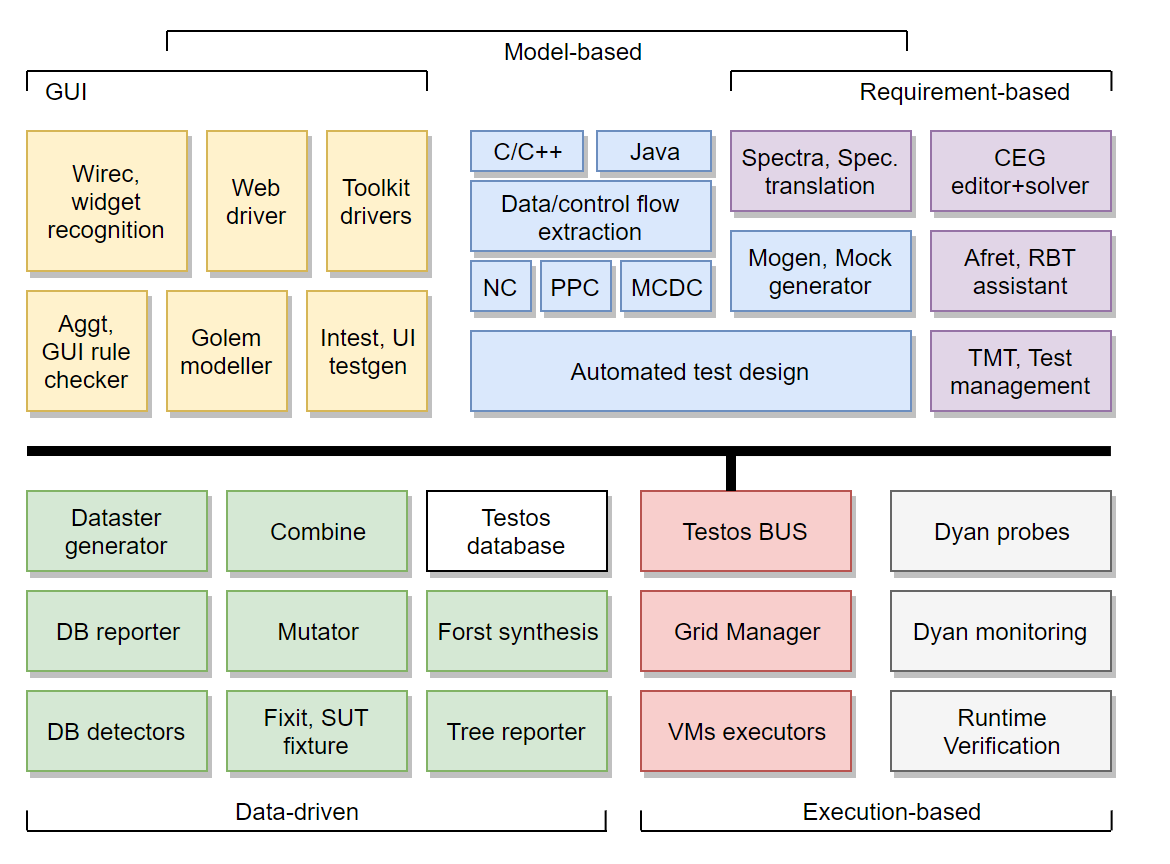
\includegraphics[width=1\textwidth]{obrazky-figures/testos.png}
	\caption{Přehled nástrojů platformy Testos}
	\label{fig_testos}
\end{figure}


\chapter{Vstupní a konfigurační soubory}
\label{chap_VstupAplikace}


\section*{Ukázka konfiguračního souboru}
\label{chap_ConfigFile}

\definecolor{maroon}{rgb}{0.5,0,0}
\definecolor{darkgreen}{rgb}{0,0.5,0}
\definecolor{darkbrown}{RGB}{139,69,19}
\definecolor{darkblue}{RGB}{25,25,112}

\lstdefinelanguage{INI}
{
  % basicstyle=\ttfamily\footnotesize,
  morecomment=[l]{;},
  morecomment=[s][\color{darkblue}\bfseries]{[}{]},
  moredelim=[s][\color{darkbrown}]{=}{\ },
  commentstyle=\color{darkgreen},
  keywordstyle={\color{maroon}\bfseries},
  morekeywords={param,parameter,parameter2},
  numbers=left,
  xleftmargin=2em,
}

\begin{lstlisting}[language={INI}, frame=single]
[ENDPOINT]
url_enum_start = <
url_enum_end = >
url_enum_separator = ,
url_variable_start = <:
url_varaible_end = :>
[METHOD]
method_enum_start = <
method_enum_end = >
method_enum_separator = ,
method_variable_start = <:
method_variable_end = :>
[HEADER]
header_enum_start = <
header_enum_end = >
header_enum_separator = ,
header_variable_start = <:
header_variable_end = :>
[BODY]
body_enum_start = <
body_enum_end = >
body_enum_separator = ,
inside_body_separator = ;
body_variable_start = <:
body_variable_end = :>
[GENERAL]
default_framework = Pytest
default_input_file = ../input/input_file.json
default_output_folder = ./result/
[COMBINATION_LIMIT]
final_tc_limit = 150
\end{lstlisting}


\section*{Ukázka vstupního soubor}

\definecolor{delim}{RGB}{20,105,176}
\definecolor{numb}{RGB}{106, 109, 32}
\definecolor{string}{rgb}{0.64,0.08,0.08}


% \lstdefinelanguage{INI}
% {
%   % basicstyle=\ttfamily\footnotesize,
%   morecomment=[l]{;},
%   morecomment=[s][\color{darkblue}\bfseries]{[}{]},
%   moredelim=[s][\color{darkbrown}]{=}{\ },
%   commentstyle=\color{darkgreen},
%   keywordstyle={\color{maroon}\bfseries},
%   morekeywords={param,parameter,parameter2},
%   numbers=left,
%   xleftmargin=2em,
% }

\lstdefinelanguage{json}{
    numbers=left,
    xleftmargin=2em,
    frame=single,
    rulecolor=\color{black},
    showspaces=false,
    showtabs=false,
    breaklines=true,
    postbreak=\raisebox{0ex}[0ex][0ex]{\ensuremath{\color{gray}\hookrightarrow\space}},
    breakatwhitespace=true,
    upquote=true,
    morestring=[b]",
    stringstyle=\color{string},
    literate=
     *{0}{{{\color{numb}0}}}{1}
      {1}{{{\color{numb}1}}}{1}
      {2}{{{\color{numb}2}}}{1}
      {3}{{{\color{numb}3}}}{1}
      {4}{{{\color{numb}4}}}{1}
      {5}{{{\color{numb}5}}}{1}
      {6}{{{\color{numb}6}}}{1}
      {7}{{{\color{numb}7}}}{1}
      {8}{{{\color{numb}8}}}{1}
      {9}{{{\color{numb}9}}}{1}
      {\{}{{{\color{delim}{\{}}}}{1}
      {\}}{{{\color{delim}{\}}}}}{1}
      {[}{{{\color{delim}{[}}}}{1}
      {]}{{{\color{delim}{]}}}}{1},
}

\begin{lstlisting}[language={json}]
{
	"test_sequence": [
		{
			"endpoint": {
		    	"values": "http://127.0.0.1:5000/api/v1/calculator",
			    "local_params": []
		    },
		    "method": {
				"values": "<:method:>",
				"local_params": []
			},
			"header": {
				"values": "<>",
				"local_params": [
					{
						"values": ["header.yaml"]
					}
				]
			},
			"body": {
				"values": "",
				"local_params": []
			},
			"t-way": 2
		}
	],
	"t-way": 2,
	"global_params": {
		"method": ["GET","POST"]
	}
}
\end{lstlisting}

% \chapter{Výstup aplikace}
% \begin{lstlisting}[language=Python, frame=single, numbers=left, xleftmargin=2em]
% from unittest import TestCase
% from json import dumps
% import requests

% class ContextClass(object):
%     def __init__(self, request, endpoint_params, method_params, header_params, body_params):
%         self.endpoint = request[0]
%         self.method = request[1]
%         self.header = request[2]
%         self.body = request[3]
%         # parameters
%         self.endpoint_params = endpoint_params
%         self.method_params = method_params
%         self.header_params = header_params
%         self.body_params = body_params

% def setup():
%     #####################################
%     # TODO: HERE IS YOUR CODE
%     # Insert your code to define prerequisities of SUT
%     None

% def verify(test_case, request_id, response, context):
%     """
%     Method to describe the expected values for all test cases
%     Take into account that these if-else statements will be duplicated for all test cases
%     You can also rewrite whole method from scretch and use [TODO:] argument while calling 
%     suiter to avoid code duplicate 
%     """
%     if test_case == "test_case_001":
%         if request_id == "call_1":
%             # Test Case Information
%             # endpoint = http://127.0.0.1:5000/api/v1/calculator?operation=add&num1=0&num2=0
%             # method = GET
%             # header = {"Content-type": "json", "testInt": "12", "dalsiTest": "test"}
%             # body = ./body_files/request_1_body_1
%             assert response.status_code == 200
%         elif request_id == "call_2":
%             # Test Case Information
%             # endpoint = http://127.0.0.1:5000/api/v1/calculator?operation=add&num1=0&num2=0
%             # method = GET
%             # header = {"Content-type": "json", "testInt": "12", "dalsiTest": "test"}
%             # body = ./body_files/request_2_body_1
%             assert response.status_code == 200
%         else:
%             raise Exception("Should have never gotten here: [{},{}]".format(test_case,request_id))

% def teardown():
%     #####################################
%     # TODO: HERE IS YOUR CODE
%     # Write a code to set the SUT to it's original state
%     # if it is dependend on given test_case, add a 'test_case' parameter to this function
%     # and write a code for all test_cases
%     ## def teardown(test_case):
%     None

% def all_test_cases(test_case, request_id):
%     """
%     List of all test cases in this test suite
%     """
%     if test_case == "test_case_001":
%         if request_id == "call_1":
%             url = "http://127.0.0.1:5000/api/v1/calculator?operation=add&num1=0&num2=0"
%             method = "GET"
%             header = {"Content-type": "json", "testInt": "12", "dalsiTest": "test"}
%             body = "./body_files/request_1_body_1"
%         elif request_id == "call_2":
%             url = "http://127.0.0.1:5000/api/v1/calculator?operation=add&num1=0&num2=0"
%             method = "GET"
%             header = {"Content-type": "json", "testInt": "12", "dalsiTest": "test"}
%             body = "./body_files/request_2_body_1"
%         else:
%             raise Exception("Should have never gotten here: [{},{}]".format(test_case,request_id))
%     else:
%         raise Exception("Should have never gotten here: [{},{}]".format(test_case,request_id))

%     return (url, method, header, body)

% class TestClass(TestCase): 
%     def test_sequence_001(self):
%         ### SUT Setup ###
%         setup()
%         ### 1. Request ###
%         call = all_test_cases("test_case_001", "call_1")
%         with open(call[3],'rb') as payload:
%             response = requests.request(call[1], call[0], headers=call[2], data=payload)
%         verify("test_case_001", "call_1", response, call)
%         ### 2. Request ###
%         call = all_test_cases("test_case_001", "call_2")
%         with open(call[3],'rb') as payload:
%             response = requests.request(call[1], call[0], headers=call[2], data=payload)
%         verify("test_case_001", "call_2", response, call)
%         ### SUT Teardown ###
%         teardown()
% \end{lstlisting}





\chapter{Šablona testovacího skriptu pro Python}
\label{cahp_sablona}

\definecolor{maroon}{rgb}{0.5,0,0}
\definecolor{darkgreen}{rgb}{0,0.5,0}
\definecolor{darkbrown}{RGB}{139,69,19}
\definecolor{darkblue}{RGB}{25,25,112}

\begin{lstlisting}[language=Python, basicstyle=\ttfamily\scriptsize,numbers=left,xleftmargin=2em,frame=single]
from unittest import TestCase
from json import dumps
import requests

class ContextClass(object):
    def __init__(self, request, endpoint_params, method_params, header_params, body_params):
        self.endpoint = request[0]
        self.method = request[1]
        self.header = request[2]
        self.body = request[3]
        # parameters
        self.endpoint_params = endpoint_params
        self.method_params = method_params
        self.header_params = header_params
        self.body_params = body_params

def setup():
    #####################################
    # TODO: HERE IS YOUR CODE
    # Insert your code to define prerequisities of SUT
    None

def verify(test_case, request_id, response, context):
    """ Method to describe the expected values for all test cases """
<VERIFY>    
    
def teardown():
    #####################################
    # TODO: HERE IS YOUR CODE
    # Write a code to set the SUT to it's original state
    None

def all_test_cases(test_case, request_id):
    """ List of all test cases in this test suite """
<TEST_CASE_LIST>
    return (url, method, header, body)

class TestClass(TestCase): 
<TEST_SEQUENCE>
\end{lstlisting}


\chapter{Obsah těla HTTP požadavku odeslaného nástroji Combine}
\label{combine_body}

\definecolor{delim}{RGB}{20,105,176}
\definecolor{numb}{RGB}{106, 109, 32}
\definecolor{string}{rgb}{0.64,0.08,0.08}

\lstdefinelanguage{json}{
    numbers=left,
    xleftmargin=2em,
    frame=single,
    rulecolor=\color{black},
    showspaces=false,
    showtabs=false,
    breaklines=true,
    postbreak=\raisebox{0ex}[0ex][0ex]{\ensuremath{\color{gray}\hookrightarrow\space}},
    breakatwhitespace=true,
    upquote=true,
    morestring=[b]",
    stringstyle=\color{string},
    literate=
     *{0}{{{\color{numb}0}}}{1}
      {1}{{{\color{numb}1}}}{1}
      {2}{{{\color{numb}2}}}{1}
      {3}{{{\color{numb}3}}}{1}
      {4}{{{\color{numb}4}}}{1}
      {5}{{{\color{numb}5}}}{1}
      {6}{{{\color{numb}6}}}{1}
      {7}{{{\color{numb}7}}}{1}
      {8}{{{\color{numb}8}}}{1}
      {9}{{{\color{numb}9}}}{1}
      {\{}{{{\color{delim}{\{}}}}{1}
      {\}}{{{\color{delim}{\}}}}}{1}
      {[}{{{\color{delim}{[}}}}{1}
      {]}{{{\color{delim}{]}}}}{1},
}

\begin{lstlisting}[language={json}]
{
    "name": "SUT name",
    "t_strength": "2",
    "dont_care_values": "no",
    "values": "values",
    "parameters": [
        {
            "identificator": "ArrayType",
            "type": "enum",
            "blocks": [
                "[1,2,3]",
                "[a,b,c]",
                "[A,B,C]"
            ]
        },
        {
            "identificator": "IntegerType",
            "type": "enum",
            "blocks": [
                "1",
                "2"
            ]
        }
    ],
    "constraints": []
}
\end{lstlisting}
  \fi
  
  % Kompilace po částech (viz výše, nutno odkomentovat)
  % Compilation piecewise (see above, it is necessary to uncomment it)
  %\subfile{projekt-30-prilohy-appendices}
  
\end{document}
